% **************************************************
% Document Class Definition
% **************************************************
\documentclass[%
	paper=A4,					% paper size --> A4 is default in Germany
	twoside=true,				% onesite or twoside printing
	openright,					% doublepage cleaning ends up right side
	parskip=full,				% spacing value / method for paragraphs
	chapterprefix=true,			% prefix for chapter marks
	12pt,						% font size
	headings=normal,			% size of headings
	bibliography=totoc,			% include bib in toc
	listof=totoc,				% include listof entries in toc
	titlepage=on,				% own page for each title page
	captions=tableabove,		% display table captions above the float env
	draft=false,				% value for draft version
]{scrreprt}%

% **************************************************
% Debug LaTeX Information
% **************************************************
%\listfiles

% **************************************************
% Information and Commands for Reuse
% **************************************************
\newcommand{\thesisTitle}{Thesis Title}
\newcommand{\thesisName}{Thesis Author}
\newcommand{\thesisSubject}{Thesis Subject}
\newcommand{\thesisDate}{March 2014}
\newcommand{\thesisVersion}{0.1}

\newcommand{\thesisFirstReviewer}{First Reviewer}
\newcommand{\thesisFirstReviewerUniversity}{\protect{The Hong Kong Polytechnic University}}
\newcommand{\thesisFirstReviewerDepartment}{Department of Computing}

\newcommand{\thesisSecondReviewer}{Second Reviewer}
\newcommand{\thesisSecondReviewerUniversity}{\protect{The Hong Kong Polytechnic University}}
\newcommand{\thesisSecondReviewerDepartment}{Department of Computing}

\newcommand{\thesisFirstSupervisor}{Prof. John Doe}

\newcommand{\thesisUniversity}{\protect{The Hong Kong Polytechnic University}}
\newcommand{\thesisUniversityDepartment}{Department of Computing}
\newcommand{\thesisUniversityInstitute}{Thesis Research Centre}
\newcommand{\thesisUniversityCity}{Hong Kong}
\newcommand{\thesisUniversityStreetAddress}{Hung Hom, Kowloon}


% **************************************************
% Load and Configure Packages
% **************************************************
\usepackage[utf8]{inputenc}		% defines file's character encoding
\usepackage[english]{babel} % babel system, adjust the language of the content
\usepackage[					% clean thesis style
	figuresep=colon,%
	sansserif=false,%
	hangfigurecaption=false,%
	hangsection=true,%
	hangsubsection=true,%
	colorize=full,%
	colortheme=bluemagenta,%
]{cleanthesis}

\hypersetup{					% setup the hyperref-package options
	pdftitle={\thesisTitle},	% 	- title (PDF meta)
	pdfsubject={\thesisSubject},% 	- subject (PDF meta)
	pdfauthor={\thesisName},	% 	- author (PDF meta)
	plainpages=false,			% 	- 
	colorlinks=false,			% 	- colorize links?
	pdfborder={0 0 0},			% 	-
	breaklinks=true,			% 	- allow line break inside links
	bookmarksnumbered=true,		%
	bookmarksopen=true			%
}


\usepackage{bm}
\usepackage{amsmath}
\usepackage{amssymb}

%\usepackage{epsfig}
%\usepackage{graphicx}
%\usepackage{url}
%\usepackage{subfigure}
%\usepackage{lineno}
%\usepackage{setspace}
%\usepackage{upgreek}
%\usepackage[numbers,sort]{natbib}
%\usepackage{authblk}
%\usepackage{xpatch}

% **************************************************
% Document CONTENT
% **************************************************
\begin{document}

% --------------------------
% rename document parts
% --------------------------
%\renewcaptionname{ngerman}{\figurename}{Abb.}
%\renewcaptionname{ngerman}{\tablename}{Tab.}
\renewcaptionname{english}{\figurename}{Fig.}
\renewcaptionname{english}{\tablename}{Table}

% --------------------------
% Front matter
% --------------------------
\pagenumbering{roman}			% roman page numbing (invisible for empty page style)
%\pagestyle{empty}				% no header or footers
%% !TEX root = ../XJ_thesis.tex
%
% ------------------------------------  --> cover title page
\begin{titlepage}
	\pdfbookmark[0]{Cover}{Cover}
	\flushright
	\hfill
	\vfill
	{\LARGE\thesisTitle} \par
	\rule[5pt]{\textwidth}{.4pt} \par
	{\Large\thesisName}
	\vfill
	\textit{\large\thesisDate} \\
	Version: \thesisVersion
\end{titlepage}


% ------------------------------------  --> main title page
\begin{titlepage}
	\pdfbookmark[0]{Titlepage}{Titlepage}
	\tgherosfont
	\centering
	
	{\Large \thesisUniversity} \\[4mm]
	
\includegraphics[width=6cm]{gfx/PolyU_Logo_CMKY} \\[2mm]
	\textsf{\thesisUniversityDepartment} \\
	\textsf{\thesisUniversityInstitute} \\
	%\textsf{\thesisUniversityGroup} \\
	
	\vfill
	{\large \thesisSubject} \\[5mm]
	{\LARGE \color{ctcolormain}\textbf{\thesisTitle} \\[10mm]}
	{\Large \thesisName} \\
	
	\vfill
	\begin{minipage}[t]{.27\textwidth}
		\raggedleft
		\textit{1. Reviewer}
	\end{minipage}
	\hspace*{15pt}
	\begin{minipage}[t]{.65\textwidth}
		{\Large \thesisFirstReviewer} \\
	  	{\small \thesisFirstReviewerDepartment} \\[-1mm]
		{\small \thesisFirstReviewerUniversity}
	\end{minipage} \\[5mm]
	\begin{minipage}[t]{.27\textwidth}
		\raggedleft
		\textit{2. Reviewer}
	\end{minipage}
	\hspace*{15pt}
	\begin{minipage}[t]{.65\textwidth}
		{\Large \thesisSecondReviewer} \\
	  	{\small \thesisSecondReviewerDepartment} \\[-1mm]
		{\small \thesisSecondReviewerUniversity}
	\end{minipage} \\[10mm]
	\begin{minipage}[t]{.27\textwidth}
		\raggedleft
		\textit{Supervisor}
	\end{minipage}
	\hspace*{15pt}
	\begin{minipage}[t]{.65\textwidth}
		\thesisFirstSupervisor%\ and \thesisSecondSupervisor
	\end{minipage} \\[10mm]
	
	\thesisDate \\
	
\end{titlepage}


% ------------------------------------  --> lower title back for single page layout
\hfill
\vfill
\small
\textbf{\thesisName} \\
\textit{\thesisTitle} \\
\thesisSubject, \thesisDate \\
Reviewers: \thesisFirstReviewer\ and \thesisSecondReviewer \\
Supervisor: \thesisFirstSupervisor \\[1.5em]
\textbf{\thesisUniversity} \\
\textit{\thesisUniversityInstitute} \\
\thesisUniversityDepartment \\
\thesisUniversityStreetAddress, \thesisUniversityCity
		% INCLUDE: all titlepages
%\cleardoublepage

\thesistitlepage{Doctor of Philosophy}%{Temporary Binding for Examination Purposes}
%\thesistitlepage{Master of Philosophy}%{Temporary Binding for Examination Purposes}
\cleardoublepage


\pagestyle{plain}				% display just page numbers
\declaration
\cleardoublepage

% !TEX root = ../thesis_phd.tex
%
\pdfbookmark[0]{Abstract}{Abstract}
\chapter*{Abstract}
\label{sec:abstract}
\vspace*{-10mm}

The nonlocal self-similarity (NSS) prior of natural images has been extensively studied in many image restoration methods. In this thesis, we exploit the NSS property of external natural images, external guided internal NSS property, and internal NSS property for image denoising tasks.

		% INCLUDE: the abstracts (english and german)
\cleardoublepage
%
% !TEX root = ../XJ_thesis.tex
%
\pdfbookmark[0]{Acknowledgement}{Acknowledgement}
\chapter*{Acknowledgement}
\label{sec:acknowledgement}
\vspace*{-10mm}

\blindtext
 % INCLUDE: acknowledgment
\cleardoublepage
%
\setcounter{tocdepth}{2}		% define depth of toc
\tableofcontents				% display table of contents
\cleardoublepage

\listoffigures
\cleardoublepage

\listoftables
\cleardoublepage

% --------------------------
% Body matter
% --------------------------
\pagenumbering{arabic}			% arabic page numbering
\setcounter{page}{1}			% set page counter
\pagestyle{maincontentstyle} 	% fancy header and footer


% !TEX TS-program = pdflatex
% !TEX root = ../thesis.tex
%
\chapter{Introduction}
\label{sec:intro}

%\cleanchapterquote{"Mens cujusque is est Quisque" – "Mind Makes the Man"}{Samuel Pepys}{}


Nowadays, CCD or CMOS cameras are becoming more and more important in many aspects of human life such as photography, artificial intelligence, and security system. For each camera product, the camera imaging pipeline in the camera is of particular importance since it is the core part to transform the real scenes into the images or videos. However, during the imaging process, the noise is unavoidablely generated due to many reasons.

\section{The Camera Imaging Pipeline}
\label{sec:intro:general}

The cameras capture the images and store as raw image formats. During the camera imaging pipeline, the photons are transformed into electronics by the photodiode in the camera sensor. The original sensor arrat (also called color filter array, or CFA) contains red, green, and blue channels, and these incomplete channels are transformed into the final RGB files via the raw converter. The camera imaging pipeline includes multiple stages such as reading raw image, black light subtraction, lens correction, demosaicing, noise reduction, white balancing, gamma curve, final color space conversion, etc \cite{browneccv2016}. Basically, a camera imaging pipeline includes demosaicing, white balancing and color space transform, gamut mapping, tone mapping, and JPEG compression \cite{crosschannel}. However, different cameras have varying structures and camera parameters, and hence resulting different imaging effects. Recently, there also exists learning based imaging pipelines which directly learn the  natural image priors from the RGB and raw images pairs.


\section{The Image Noise}
\label{sec:intro:current}

In image denoising community, the most commonly studied noise is the additive white Gaussian noise, which is used to model the independent noise in the raw images. The AWGN noise is described as a Gaussian distribution $\mathcal{N}(0,\sigma^{2})$, which means that the noise is Gaussian distributed with $0$ mean and $\sigma$ standard deviation. Most of methods are focus on this type of noise since it is a good testing bed for many other image restoration problems such as super-resolution, deblurring, inpainting, etc.

However, the realistic noise in real-world natural images captured by cameras are much more complex than the synthetic AWGN noise being widely studied. The major reason is that, during the imaging pipeline, the noise will be generated. The key reason of noise generation is unstable measurement from the discrete nature of light and the thermal agitation. The major sources of noise generated during the imaging pipeline are the random noise , the spatial non-uniformity, and quantization noise. The random noise includes photon shot noise, dark current, and readout noise. The spatial non-uniformity noise includes the fixed pattern noise (PRNU, DCNU), CCD/CMOS specific noise. 


A simplified model including various noise sources (for each pixel) can be approximately defined as follows:
\begin{equation}
\bm{P} = f((g_{cv}(\bm{C}+\bm{D})+\bm{N}_{reset})g_{out}+\bm{N}_{out})+\bm{Q}.
\end{equation}
Now the above equation is explained in details. 
$\bm{P}$ is the raw pixel value, 
$\bm{C}$ is the number of absorbed electrons (charges) transformed from the photons via the photon-diodes in the camera sensor,
$\bm{D}$ is the number of absorbed electrons generated by dark current,
$g_{cv}$ is the equivalent capacitance (EC) of the photo-diode,
$\bm{N}_{reset}$ is the thermal noise generated by the readout circuitry (or reset noise related to reset voltage),
$g_{out}$ is the gain factor during voltage to pixel value conversion (readout),
$\bm{N}_{out}$ is the readout noise,
$f$ is the camera response function, usually a linear function before attaining a saturation threshold,
$\bm{Q}$ is the quantization error happened during rounding to interger values. The quantization noise is normally negligible compared to the readout noise.

Though can be approximated as Gaussian or Poisson distribution, these noise sources will be largely changed to be more complex during the in-camera imaging pipeline, which has been analyzed in \cite{crosschannel}. Hence, the real-world noise is much more complex than the traditional additive white Gaussian noise, and should be paid more attention.

In order to obtain good images while still maintaining the structures and details of the captured scene, image denoising is a good choice. In this thesis, I will present my work on image denoising, including synthetic noisy images and real noisy images. Note that the realistic noise in real color noisy images are much more complex than the usually synthetic additive white Gaussian noise (AWGN). This is because that during the camera imaging pipeline, the noise generated will be modified to be more complex than the noise in the raw sensor data. Hence, in this thesis, we pay more attention to the realistic noise generated during the camera imaging pipeline. 


\section{The Proposed Methods}
\label{sec:intro:new}

This thesis is made up of several work I have done during my study, in which I focus on designing new and better image denoising algorithms. 

Firstly, we propose a method for denoising synthetic AWGN noise, from which we can study the performance of the nonlocal self-similarity priors of natural images. In fact, we propose to learn the external NSS priors and apply the learned model on denoising AWGN noise. The proposed method achieves state-of-the-art performance on AWGN denoising on both effectiveness and efficiency. 

Basing on the success on the synthetic noise removal, I propose to exploit the power of the NSS priors in natural images to deal with the complex realistic noise in real-world noisy images. Specifically, we propose three methods exploiting the NSS priors of natural images for real noisy image denoising, which can be introduced as follows.

In the first method, I propose to learn the NSS prior from the external natural images, and then apply the learned external prior to guide the learning of the internal NSS prior of the input real noisy image. The experiments on two commonly used datasets and a new one we constructed to implement the shortage of existing datasets, demonstrate that the proposed method can achieve better performance than existing color image denoising methods such as CBM3D \cite{cbm3d}, the state-of-the-art Gaussian noise removal methods \cite{bm3d,mlp,csr}, and the real noisy image denoising methdos \cite{} including a commercial software Neat Image \cite{neatimage}, which is embeded into the famous PhotoShop CS for image processing tasks.


In the second method, I propose to employ the low rank model describe fully the the internal NSS prior, basing on the observed fact that the similar image patches can be contanated as a matrix of low rank. Different from the previous work, I extend the WNNM model and apply it to multi-channel version to make it feasible for color image denoising. 

In the third method,  is to use the sparse coding based method with additional weighting scheme to regard the local noise in real noisy images as a Gaussian and the prior is used to deal with the real noisy image.

Finally, to make my thesis more comprehensive, I construct a large benchmark of real noisy images captured by different types of famous commercial cameras, on which I also evaluate the image denoising methods mentioned above and the proposed methods in this thesis. 




The structure of this thesis is organized as follows: in the chapter 2, we review the literatures in the image denoising area; in the chapter 3, we introduce the fully external method; in the chapter 4, we introduce the external prior guided internal method; in the chapter 5, we introduce the internal method based on low ran model; in the chapter 6, we introduce the internal method based on sparse coding model; in the chapter 7, we introduce the real noisy image dataset we construct, and finaly evaluate the proposed methods with the compared competing methods, both for synthetic AWGN or Poisson noise and real noise, including the commercial software designed especially for real noise. 


\section{Thesis Structure}
\label{sec:intro:structure}


\textbf{Chapter \ref{sec:review}: Literature Review} \\[0.2em]

In this chapter, we review the related work and give a detailed introduction of the literature. We will first review the most representative work on additive white Gaussian noise removal. I review the detailed work on camera imaging pipeline and realistic noise generated in the camera sensors. I will also review the work on real noisy image denoising.



\textbf{Chapter \ref{sec:external}: External Nonlocal Self-Similarity Prior Learning for Synthetic Gaussian Noise Removal} \\[0.2em]

In this chapter, I will introduce our work on external nonlocal self-similarity (NSS) prior learning for synthetic Gaussian noise removal. As far as we know, this work is the first to learn the NSS priors of natural clean images, while previous work only utilize the NSS priors of input noisy image for online denoising. The advantages of this offline learning is that it can preserve the details of natural images while being much faster then most online denoising methods.


\textbf{Chapter \ref{sec:guided}: External Prior Guided Internal Prior Learning for Real Noisy Image Denoising} \\[0.2em]

In this chapter, I will introduce our work on external prior guided internal prior learning method for real noisy image denoising. This work can maintain the advantages of both sides: from the external perspective, the method can preserve the structures of natural images better than the internal methods, while from the perspective of internal method, the proposed method can recover the details of the input noisy image better than the external methods.



\textbf{Chapter \ref{sec:internallr}: Multi-channel Weighted Nuclear Norm Minimization for Real Color Image Denoising} \\[0.2em]

In this chapter, we introduce a multi-channel weighted nuclear norm minimization (MC-WNNM) method. This method regards different channels in RGB images differently to adaptively process the real color noisy images. Besides, this work also propose a new strategy for color image denoising. Experiments demonstrate that the proposed method can achieve better performance on real color image denoising than existing state-of-the-art methods, including some commercial software.



\textbf{Chapter \ref{sec:internalsc}: A Triple Weighted Sparse Coding Scheme for Realistic Noisy Image Denoising} \\[0.2em]

In this chapter, I introduce a novel sparse coding based method for real color image denoising. In this method, I regard the noise in each of the local region in the real noisy image as a Gaussian, and propose a triplely weighted scheme to deal with the complex realistic noise in real color noisy images. Experiments show that the proposed method performs better and faster than the nuclear norm based method mentioned in previous chapter.


\textbf{Chapter \ref{sec:dataset}: A Benchmark on Real Color Noisy Image, with Comprehensive Evaluation of State-of-the-art} \\[0.2em]

To fully boost the research of real color noisy image denoising, we construct a large benchmark on real color noisy images. This dataset is collected from several representative cameras with comprehensive settings on contents, lighting, ISO, shutter, and aperture, etc. Based on this newly established dataset, we fully evaluated existing denoising methods, including the methods designed for synthetic Gaussian noise and the methods designed especially for real color noise. We believe that this new dataset will largely boost the research of the image denoising especially the realistic image denoising problems.
















 % INCLUDE: introduction
%% !TEX root = ../thesis.tex
%
\chapter{Literature Review}
\label{sec:review}

\cleanchapterquote{"Mens cujusque is est Quisque" – "Mind Makes the Man"}{Samuel Pepys}{}

\blindtext

\section{System}
\label{sec:review:sys}

\blindtext

\section{Feature Extraction}
\label{sec:review:feature}

\blindtext
 % INCLUDE: literature-review
% !TEX root = ../thesis.tex
%
\chapter{Literature Review}
\label{sec:review}

\cleanchapterquote{"Mens cujusque is est Quisque" – "Mind Makes the Man"}{Samuel Pepys}{}

\blindtext

\section{System}
\label{sec:review:sys}

\blindtext

\section{Feature Extraction}
\label{sec:review:feature}

\blindtext
 % INCLUDE: literature-review
% !TEX root = ../XJ_thesis.tex
%
\chapter{External Prior Guided Internal Prior Learning for Real Noisy Image Denoising}
\label{sec:guided}

\section{Introduction}
\label{sec:system:intro}

Image denoising is a crucial and indispensable step to improve image quality in digital imaging systems. In particular, with the decrease of size of CMOS/CCD sensors, image is more easily to be corrupted by noise and hence denoising is becoming increasingly important for high resolution imaging. The problem of image denoising has been extensively studied in literature and numerous image denoising methods
\cite{bayesshrink,curvelet,ksvd,lssc,ncsr,bm3d,cbm3d,
zhou2012nonparametric,Tomasi1998,blsgsm,nlm,nlbayes,wnnm,pgpd,combexin,external,
tid,foe,epll,
mlp,xie2012image,dncnn,
barbu2009training,csf,tnrd,Fadili,salmon2014,
Foipractical,Luisier,makitalo2013optimal,Montagner,
jiang2014mixed,Hu2016,xuaccv2016,
fullyblind,rabie2005robust,Liu2008,almapg,noiseclinic,
ncwebsite,Zhu_2016_CVPR,crosschannel2016,neatimage}
have been proposed in the past decades. Most of existing denoising methods focus on the scenario of additive white Gaussian noise (AWGN) 
\cite{bayesshrink,curvelet,ksvd,lssc,ncsr,bm3d,cbm3d,
zhou2012nonparametric,Tomasi1998,blsgsm,nlm,nlbayes,wnnm,pgpd,foe,epll,
mlp,xie2012image,dncnn,barbu2009training,csf,tnrd}, where the observed noisy image $\mathbf{y}$ is modeled as the addition of clean image $\mathbf{x}$ and AWGN $\mathbf{n}$, i.e., $\mathbf{y}=\mathbf{x}+\mathbf{n}$. There are also methods proposed for removing Poisson noise \cite{Fadili,salmon2014}, mixed Poisson and Gaussian noise \cite{Foipractical,Luisier,makitalo2013optimal,Montagner}, mixed Gaussian and impulse noise \cite{jiang2014mixed,Hu2016,xuaccv2016}, and realistic noise in real photography \cite{fullyblind,rabie2005robust,Liu2008,almapg,Zhu_2016_CVPR,noiseclinic,
ncwebsite,crosschannel2016,neatimage}.

Natural images have many priors, such as sparsity and nonlocal self-similarity, which can be employed as useful priors for designing image denoising methods. Based on the facts that natural images will be sparsely distributed in some transformed domain, wavelet \cite{bayesshrink} and curvelet \cite{curvelet} transforms have been widely adopted for image denoising. The sparse representation based methods \cite{ksvd,lssc,ncsr,bm3d,cbm3d,zhou2012nonparametric} encode image patches over a dictionary by using $\ell_{1}$-norm minimization to enforce the sparsity. The well-known bilateral filters \cite{Tomasi1998} employ the prior information that image pixels exhibit similarity in both spatial domain and intensity domain. Other image priors such as multiscale self-similarity \cite{blsgsm} and nonlocal self-similarity \cite{nlm,nlbayes}, or the combination of multiple image priors \cite{wnnm,pgpd} have also been successfully used in image denoising. For example, by using low-rank minimization to characterize the image nonlocal self-similarity, the WNNM \cite{wnnm} method achieves state-of-the-art performance for AWGN denoising. 

Instead of using predefined image priors, methods have also been proposed to learn priors from natural images for denoising. The generative image prior learning methods usually learn prior models from a set of external clean images and apply the learned prior models to the given noisy image \cite{foe,epll,pgpd}, or learn priors from the given noisy image to perform denoising \cite{ksvd}. Recently, the discriminative image prior learning methods \cite{mlp,xie2012image,dncnn,tnrd,barbu2009training,csf}, which learn denoising models from pairs of clean and noisy images, have been becoming popular. The representative methods include the neural network based methods \cite{mlp,xie2012image,dncnn}, random fields based methods \cite{barbu2009training,csf}, and reaction diffusion based methods \cite{tnrd}.

Learning natural image priors plays a key role in image denoising
\cite{blsgsm,zhou2012nonparametric,ksvd,lssc,ncsr,foe,epll,pgpd,combexin,external,
tid,mlp,xie2012image,dncnn,barbu2009training,csf,tnrd}. There are mainly four categories of prior learning based methods. 1) External prior learning methods \cite{foe,epll,pgpd} learn priors (e.g., dictionaries) from a set of external clean images, and the learned priors are used to recover the latent clean image from the given noisy image. 2) Internal prior learning methods \cite{blsgsm,zhou2012nonparametric,ksvd,lssc,ncsr} directly learn priors from a given noisy image, and image denoising is often done simultaneously with the prior learning process. 3) Discriminative prior learning methods \cite{mlp,xie2012image,dncnn,barbu2009training,
csf,tnrd} learn discriminative models or mapping functions from clean and noisy image pairs, and the learned models or mapping functions are applied to a noisy image for denoising. 4) Hybrid methods \cite{combexin,external,tid} combine the external and internal priors to denoise the given input image.

\begin{figure}
    \centering
    \begin{subfigure}[t]{0.19\textwidth}
        \centering
        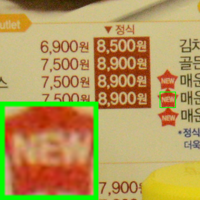
\includegraphics[width=1\textwidth]{images/guided/resize_br_Noisy_CC_Noisy_Nikon_D800_ISO_3200_A3_66.png}
	   \caption{Noisy 33.30}
    \end{subfigure}
    \hfill
    \begin{subfigure}[t]{0.19\textwidth}
        \centering
        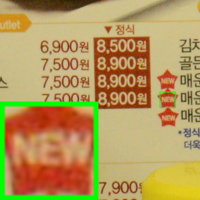
\includegraphics[width=1\textwidth]{images/guided/resize_br_CBM3D_CC_Noisy_Nikon_D800_ISO_3200_A3_66.png}
		\caption{CBM3D34.55}
    \end{subfigure}
    \hfill
    \begin{subfigure}[t]{0.19\textwidth}
        \centering
        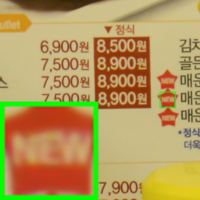
\includegraphics[width=1\textwidth]{images/guided/resize_br_WNNM_CC_Noisy_Nikon_D800_ISO_3200_A3_66.png}
		\caption{WNNM35.85}
    \end{subfigure}
    \hfill
    \begin{subfigure}[t]{0.19\textwidth}
        \centering
        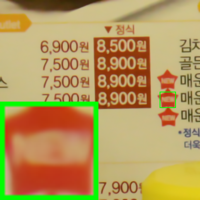
\includegraphics[width=1\textwidth]{images/guided/resize_br_CSF_CC_Noisy_Nikon_D800_ISO_3200_A3_66.png}
		\caption{CSF 35.39}
    \end{subfigure}
    \hfill
    \begin{subfigure}[t]{0.19\textwidth}
        \centering
        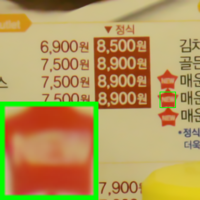
\includegraphics[width=1\textwidth]{images/guided/resize_br_TRD_CC_Noisy_Nikon_D800_ISO_3200_A3_66.png}
		\caption{TNRD 35.97}
    \end{subfigure}
    \hfill
    \begin{subfigure}[t]{0.19\textwidth}
        \centering
        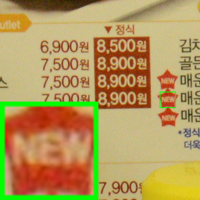
\includegraphics[width=1\textwidth]{images/guided/resize_br_DnCNN_CC_Noisy_Nikon_D800_ISO_3200_A3_66.png}
	   \caption{DnCNN34.14}
    \end{subfigure}
    \hfill
    \begin{subfigure}[t]{0.19\textwidth}
        \centering
        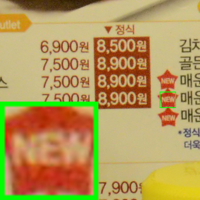
\includegraphics[width=1\textwidth]{images/guided/resize_br_NI_CC_Noisy_Nikon_D800_ISO_3200_A3_66.png}
		\caption{NI 34.39}
    \end{subfigure}
    \hfill
    \begin{subfigure}[t]{0.19\textwidth}
        \centering
        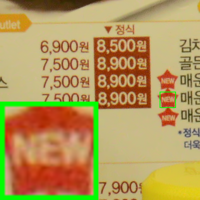
\includegraphics[width=1\textwidth]{images/guided/resize_br_NC_CC_Noisy_Nikon_D800_ISO_3200_A3_66.png}
		\caption{NC 35.33}
    \end{subfigure}
    \hfill
    \begin{subfigure}[t]{0.19\textwidth}
        \centering
        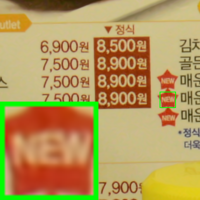
\includegraphics[width=1\textwidth]{images/guided/resize_br_Guided_CC_Noisy_Nikon_D800_ISO_3200_A3_66.png}
		\caption{Ours \textbf{37.49}}
    \end{subfigure}
    \hfill
    \begin{subfigure}[t]{0.19\textwidth}
        \centering
        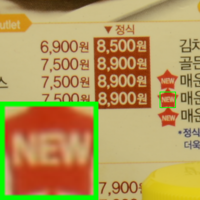
\includegraphics[width=1\textwidth]{images/guided/resize_br_Mean_CC_Noisy_Nikon_D800_ISO_3200_A3_66.png}
		\caption{Mean Image}
    \end{subfigure}
    \caption{Denoised images and PSNR (dB) results of a region cropped from the real noisy image ``Nikon D800 ISO 3200 A3'' \cite{crosschannel2016} by different methods.\ The scene was shot 500 times with the same camera and camera setting.\ The mean image of the 500 shots is roughly taken as the ``ground truth'', with which the PSNR index can be computed. The images are better viewed by zooming in on screen.}
    \label{fig3-1}
\end{figure}

It has been shown \cite{foe,epll,pgpd} that the external priors learned from natural clean images are effective and efficient for universal image denoising problems, whereas they are not adaptive to the given noisy image and some fine-scale image structures may not be well recovered. By contrast, the internal priors learned from the given noisy image are adaptive to image content, but the learned priors can be much affected by noise and the learning processing is usually slow \cite{blsgsm,zhou2012nonparametric,ksvd,lssc,ncsr}. Besides, most of the internal prior learning methods \cite{blsgsm,zhou2012nonparametric,ksvd,lssc,ncsr} assume additive white Gaussian noise (AWGN), making the learned priors less robust for real-world noisy images. In this work, we use external priors to guide the internal prior learning. Our method is not only much faster than the traditional internal learning methods, but also very robust to denoise real-world noisy images.

In \cite{combexin}, the authors employed external clean patches to denoise noisy patches with high individual Signal-to-Noise-Ratio (PatchSNR), and employed internal noisy patches to denoise noisy patches with low PatchSNR. This is essentially different from our work which employs the external patch group based prior to guide the clustering and dictionary learning of the internal noisy patch groups. In \cite{external}, the external priors are only used to guide the internal patch clustering for image denoising, while in our work, the learned external priors are employed to guide not only the internal clustering, but also the internal dictionary learning. Besides, the method of \cite{external} follows a patch based framework for AWGN removal, while in our work we employ a patch group based framework for real-world noisy image denoising. In addition, some technical details are also different. For example, method in \cite{external} utilizes low-rank minimization for denoising, while we use dictionary learning and sparse coding for denoising. In the Targeted Image Denoising (TID) method \cite{tid}, targeted images are selected from a large dataset for each patch in the input noisy image for denoising, which is computationally expensive.

Most of the denoising methods in literature \cite{bayesshrink,curvelet,ksvd,lssc,ncsr,bm3d,cbm3d,
zhou2012nonparametric,Tomasi1998,blsgsm,nlm,nlbayes,wnnm,pgpd,foe,epll,
mlp,xie2012image,dncnn,barbu2009training,csf,tnrd} assume AWGN noise and use simulated noisy images for algorithm design and evaluation. However, the assumption of AWGN is too ideal to be true for real-world noisy images, where the noise is much more complex and varies with different scenes, cameras and camera settings (ISO, shutter speed, and aperture, etc.) \cite{crosschannel2016,healey1994radiometric}. As a result, many denoising methods in literature, including those learning based methods, become less effective when applied to real-world noisy images. Fig. \ref{fig3-1} shows an example, where we apply some representative and state-of-the-art denoising methods, including CBM3D \cite{cbm3d}, WNNM \cite{wnnm}, DnCNN \cite{dncnn}, CSF \cite{csf}, and TNRD \cite{tnrd} to a real noisy image (captured by a Nikon D800 camera with ISO is 3200) provided in \cite{crosschannel2016}. One can see that these methods either remain much the noise or over-smooth the image details.

Recently, several denoising methods have been proposed to remove unknown noise from real-world noisy images \cite{fullyblind,rabie2005robust,Liu2008,almapg,crosschannel2016,Zhu_2016_CVPR,noiseclinic,ncwebsite}. Portilla \cite{fullyblind} employed a correlated Gaussian model to estimate the noise of each wavelet subband. Rabie \cite{rabie2005robust} modeled the noisy pixels as outliers and performed denoising via Lorentzian robust estimator. Liu et al. \cite{Liu2008} proposed the ``noise level function'' to estimate the noise and performed denoising by learning a Gaussian conditional random field. Gong et al. \cite{almapg} proposed to model the data fitting term via weighted sum of $\ell_{1}$ and $\ell_{2}$ norms and performed denoising by a simple sparsity regularization term in the wavelet transform domain. The ``Noise Clinic'' \cite{noiseclinic,ncwebsite} estimates the noise distribution by using a multivariate Gaussian model and removes the noise by using a generalized version of nonlocal Bayesian model \cite{nlbayes}. Zhu et al. \cite{Zhu_2016_CVPR} proposed a Bayesian method to approximate and remove the noise via a low-rank mixture of Gaussians (MoG) model. The method in \cite{crosschannel2016} models the cross-channel noise in real-world noisy image as a multivariate Gaussian and the noise is removed by the Bayesian nonlocal means filter \cite{kervrann2007bayesian}. The commercial software Neat Image \cite{neatimage} estimates the noise parameters from a flat region of the given noisy image and filters the noise correspondingly. 

There have been a few methods \cite{fullyblind,rabie2005robust,Liu2008,almapg,crosschannel2016,Zhu_2016_CVPR,noiseclinic,ncwebsite} and software toolboxes \cite{neatimage} developed for real noisy image denoising. Almost all of these methods follow a two-stage framework: first estimate the parameters of the noise model (usually assumed to be Gaussian or mixture of Gaussians (MoG)), and then perform denoising with the estimated noise model. However, the noise in real noisy images is very complex and is hard to be modeled by explicit distributions such as Gaussian and MoG. According to \cite{healey1994radiometric}, the noise corrupted in the in-camera imaging process \cite{tsin2001statistical,NewInCamera,crosschannel2016,karaimer_brown_ECCV_2016} is signal dependent and comes from five main sources: photon shot, fixed pattern, dark current, readout, and quantization noise. The existing methods \cite{fullyblind,rabie2005robust,Liu2008,almapg,crosschannel2016,Zhu_2016_CVPR,noiseclinic,
ncwebsite,neatimage} mentioned above may not perform well on real noisy image denoising tasks. Fig. \ref{fig3-1} also shows the denoising results of two real noisy image denoising methods, Noise Clinic \cite{noiseclinic,ncwebsite} and Neat Image \cite{neatimage}. One can see that these two methods still generate much noise caused artifacts. 

This work aims to develop a new paradigm for real noisy image denoising. Different from existing real noisy image denoising methods \cite{fullyblind,rabie2005robust,Liu2008,almapg,crosschannel2016,Zhu_2016_CVPR,noiseclinic,ncwebsite}  which focus on noise modeling, we focus on image prior learning. We argue that with a strong and adaptive prior learning scheme, robust denoising performance on real noisy images can still be obtained. To achieve this goal, we propose to first learn image priors from external clean images, and then employ the learned external priors to guide the learning of internal priors from the given noisy image. The flowchart of the proposed method is illustrated in Fig. \ref{fig3-2}. We first extract millions of patch groups (PGs) from a set of high quality natural images, with which a Gaussian Mixture Model (GMM) is learned as the external image prior. The learned GMM prior model is used to cluster the PGs extracted from the given noisy image, and then an external-internal hybrid orthogonal dictionary is learned as the final prior for each cluster, with which the denoising can be readily performed by weighted sparse coding with closed form solution. Our proposed denoising method is simple and efficient, yet our extensive experiments on real noisy images demonstrate its better denoising performance than the current state-of-the-arts.


\begin{figure}
\label{fig3-2}
\centering
\captionsetup{justification=centering,margin=0.1cm}
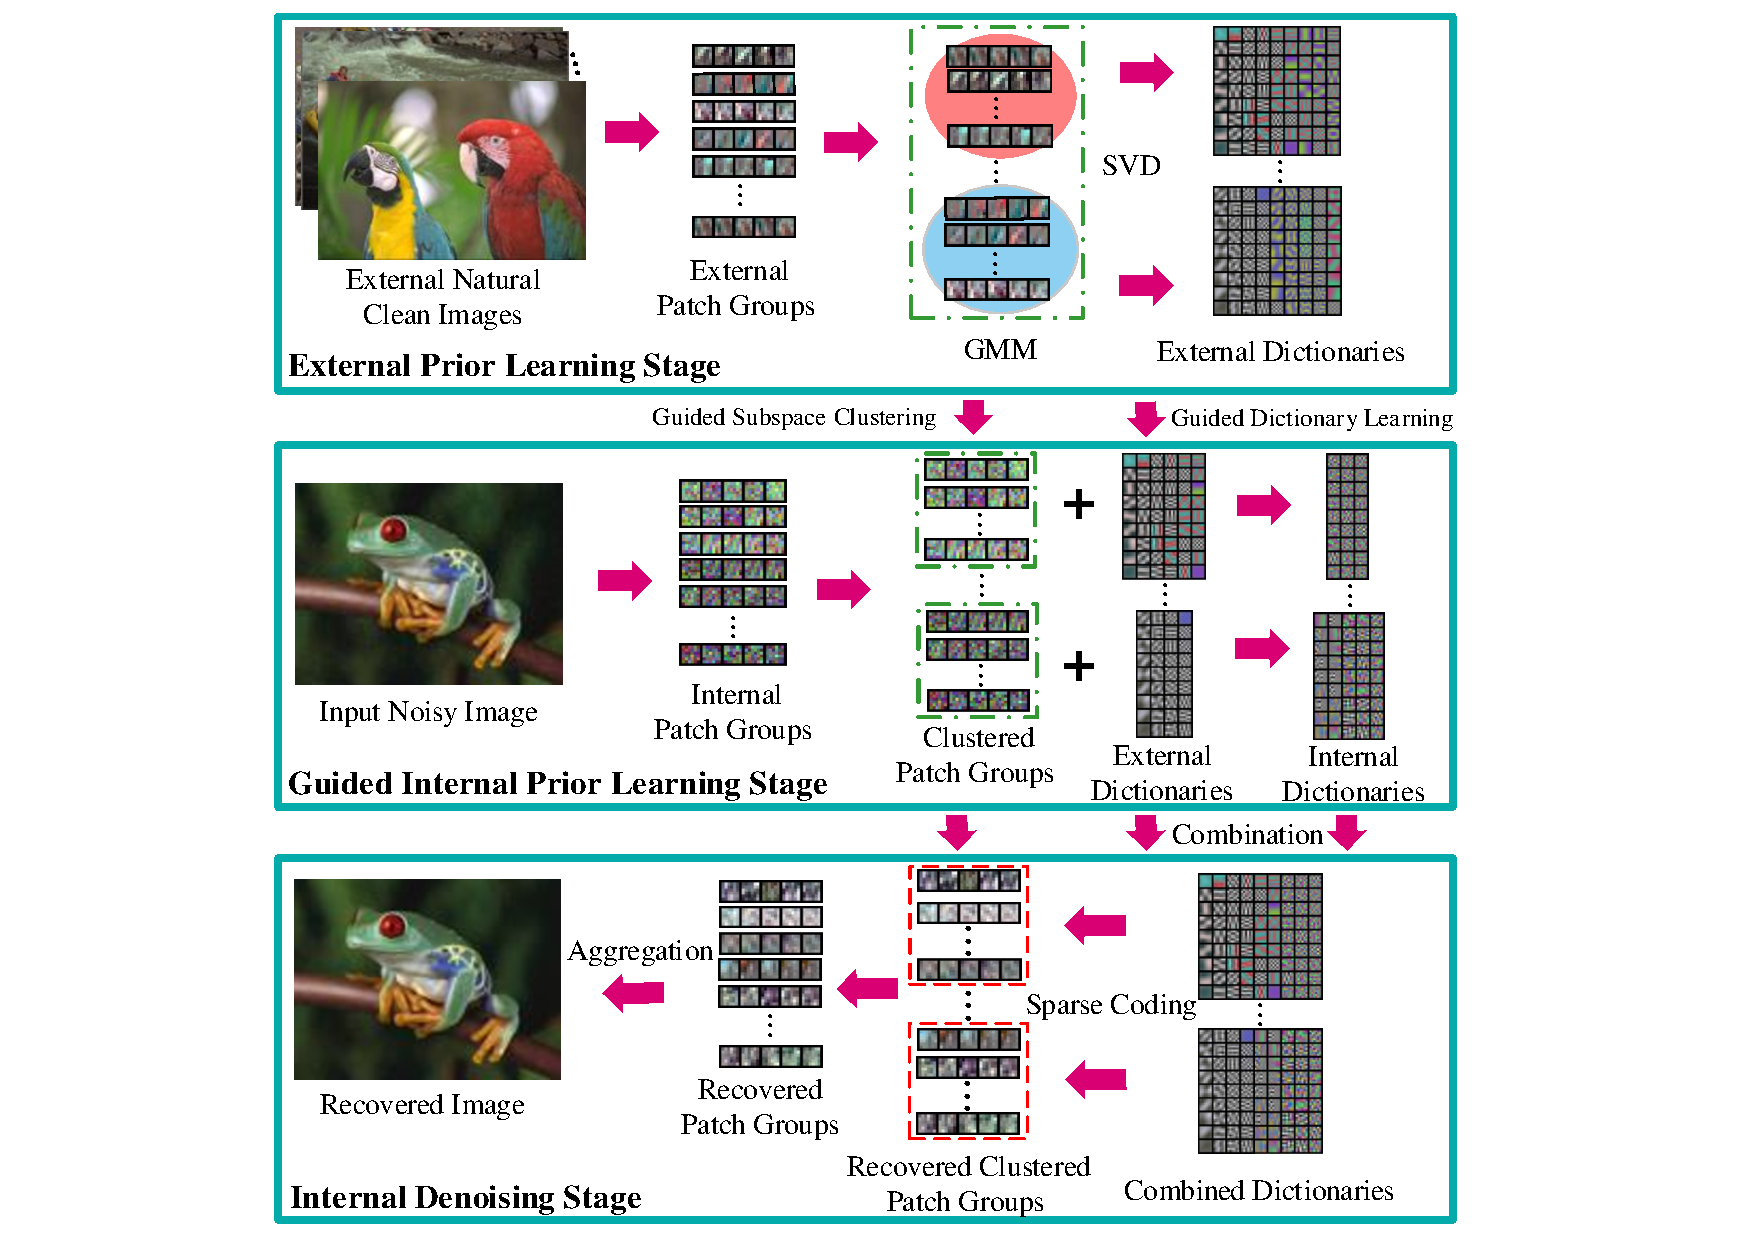
\includegraphics[width=0.8\linewidth]{images/guided/Flowchart.jpg}
\centering
\caption{Flowchart of the proposed external prior guided internal prior learning and denoising framework.}
\end{figure}



\section{External Prior Guided Internal Prior Learning for Image Denoising}

In this section, we first describe the learning of external prior, and then describe in detail the guided internal prior learning method, followed by the denoising algorithm.

\subsection{Learn External Patch Group Priors}

The nonlocal self-similarity based patch group (PG) prior learning \cite{pgpd} has proved to be very effective for image denosing. In this work, we extract PGs from natural clean images to learn external priors. A PG is a group of similar patches to a local patch. In our method, each local patch is extracted from a RGB image with patch size $p\times p \times 3$.\ We search the $M$ most similar (i.e., smallest Euclidean distance) patches to this local patch (including the local patch itself) in a $W\times W$ region around it. Each patch is stretched to a patch vector $\mathbf{x}_{m}\in \mathbb{R}^{3p^{2}\times1}$ to form the PG, denoted by $\{\mathbf{x}_{m}\}_{m=1}^{M}$.\ The mean vector of this PG is $\bm{\mu}=\frac{1}{M}\sum_{m=1}^{M}\mathbf{x}_{m}$, and the group mean subtracted PG is defined as $\mathbf{\overline{X}}\triangleq \{\mathbf{\overline{x}}_{m}=\mathbf{x}_{m}-\bm{\mu}\}_{m=1}^{M}$.

Assume that a number of $L$ PGs are extracted from a set of external natural images, and the $l$-th PG is $\mathbf{\overline{X}}_{l}\triangleq \{\mathbf{\overline{x}}_{l,m}\}_{m=1}^{M}, l=1,...,L$.\ A Gaussian Mixture Model (GMM) is learned to model the PG prior.\ The overall log-likelihood function is
\vspace{-2mm}
\begin{equation}\label{equ3-1}
\vspace{-2mm}
\begin{split}
\ln\mathcal{L}=\sum_{l=1}^{L} \ln(\sum_{k=1}^{K}\pi_{k}\prod_{m=1}^{M}\mathcal{N}(\mathbf{\overline{x}}_{l,m}|\bm{\mu}_{k},\bm{\Sigma}_{k})).
\end{split}
\end{equation}
The learning process is similar to the GMM learning in \cite{pgpd,epll}.\ Finally, a GMM model with $K$ Gaussian components is learned, and the learned parameters include mixture weights $\{\pi_{k}\}_{k=1}^{K}$, mean vectors $\{\bm{\mu}_{k}\}_{k=1}^{K}$, and covariance matrices $\{\bm{\Sigma}_{k}\}_{k=1}^{K}$.\ Note that the mean vector of each cluster is naturally zero, i.e., $\bm{\mu}_{k}=\bm{0}$.  

To better describe the subspace of each Gaussian component, we perform singular value decomposition (SVD) \cite{eckart1936approximation} on the covariance matrix:
\vspace{-2mm}
\begin{equation}\label{equ3-2}
\vspace{-2mm}
\bm{\Sigma}_{k}=\bm{U}_{k}\bm{S}_{k}\bm{U}_{k}^{\top}.
\end{equation}
The eigenvector matrices $\{\bm{U}_{k}\}_{k=1}^{K}$ will be employed as the external orthogonal dictionary to guide the internal sub-dictionary learning in next sub-section.\ The singular values in $\bm{S}_{k}$ reflect the significance of the singular vectors in $\bm{U}_{k}$.\ They  will also be utilized as prior weights for weighted sparse coding in our denoising algorithm.


\subsection{Guided Internal Prior Learning}

After the external PG prior model is learned from external natural clean images, we employ it to guide the internal PG prior learning for a given real noisy image.\ The guidance lies in two aspects. First, the external prior will guide the subspace clustering of internal noisy PGs. Second, the external prior will guide the orthogonal dictionary learning of internal noisy PGs.

\subsubsection{Internal Subspace Clustering}

Given a real noisy image $\mathbf{y}$, we extract $N$ (overlapped) local patches from it.\ Similar to the external prior learning stage, for the $n$-th ($n=1,...,N$) local patch we search its $M$ most similar (by Euclidean distance) patches around it to form a noisy PG, denoted by $\bm{Y}_{n} = \{\mathbf{y}_{n,1},...,\mathbf{y}_{n,M}\}$.\ Then the group mean of $\bm{Y}_{n}$, denoted by $\bm{\mu}_{n}$, is subtracted from each patch by $\bm{\overline{y}}_{n,m}\triangleq\mathbf{y}_{n,m}-\bm{\mu}_{n}$, leading to the mean subtracted noisy PG $\bm{\overline{Y}}_{n}\triangleq \{\bm{\overline{y}}_{n,m}\}_{m=1}^{M}$.

The external GMM prior models $\{\mathcal{N}(\bm{0},\bm{\Sigma}_{k})\}_{k=1}^{K}$ basically characterize the subspaces of natural high quality PGs.\ Therefore, we project each noisy PG $\bm{\overline{Y}}_{n}$ into the subspaces of $\{\mathcal{N}(\bm{0},\bm{\Sigma}_{k})\}_{k=1}^{K}$ and assign it to the most suitable subspace based on the posterior probability:
\vspace{-2mm}
\begin{equation}\label{equ3-3}
\vspace{-2mm}
P(k|\bm{\overline{Y}}_{n})=\frac{\prod_{m=1}^{M}\mathcal{N}(\bm{\overline{y}}_{n,m}|\bm{0},\bm{\Sigma}_{k})}{\sum_{l=1}^{K}\prod_{m=1}^{M}\mathcal{N}(\bm{\overline{y}}_{n,m}|\bm{0},\bm{\Sigma}_{l})}
\end{equation}
for $k=1,...,K$.\ Then $\bm{\overline{Y}}_{n}$ is assigned to the subspace with the maximum \emph{a}-posteriori (MAP) probability $\max_{k}P(k|\bm{\overline{Y}}_{n})$.


\subsubsection{Guided Orthogonal Dictionary Learning}

Assume that we have assigned all the internal noisy PGs $\{\bm{\overline{Y}}_{n}\}_{n=1}^{N}$ to their corresponding most suitable subspaces in $\{\mathcal{N}(\bm{0},\bm{\Sigma}_{k})\}_{k=1}^{K}$. For the $k$-th subspace, the noisy PGs assigned to it are $\{\bm{\overline{Y}}_{k_{n}}\}_{n=1}^{N_{k}}$, where $\bm{\overline{Y}}_{k_{n}}=[\bm{\overline{y}}_{k_{n},1},...,\bm{\overline{y}}_{k_{n},M}]$ and $\sum_{k=1}^{K}N_{k}=N$.\ We propose to learn an orthogonal dictionary $\bm{D}_{k}$ from each set of PGs $\bm{\overline{Y}}_{k_{n}}$ to characterize the internal PG prior with the guidance of the corresponding external orthogonal dictionary $\bm{U}_{k}$ (Eq.\ (\ref{equ2})). The reasons that we learn orthogonal dictionaries are two-fold.\ Firstly, the PGs $\{\bm{\overline{Y}}_{k_{n}}\}_{n=1}^{N_{k}}$ are in a subspace of the whole space of all PGs; therefore, there is no necessary to learn a redundant over-complete dictionary to characterize it, while an orthonormal dictionary has naturally zero \emph{mutual incoherence} \cite{donoho2001uncertainty}. Secondly, the orthogonality of dictionary can make the patch encoding in the testing stage very efficient, leading to an efficient denoising algorithm (please refer to sub-section III-C for more details).

We let the orthogonal dictionary $\bm{D}_{k}$ be 
\vspace{-2mm}
\begin{equation}
\vspace{-2mm}
\label{equ3-4}
\bm{D}_{k}\triangleq[\bm{D}_{k,\text{E}}\ \bm{D}_{k,\text{I}}]\in \mathbb{R}^{3p^2\times 3p^2},
\end{equation}
where $\bm{D}_{k,\text{E}}=\bm{U}_{k}(:,1:r)\in\mathbb{R}^{3p^2\times r}$ is the external sub-dictionary and it includes the first $r$ most important eigenvectors of $\bm{U}_{k}$, and the internal sub-dictionary $\bm{D}_{k,\text{I}}\in\mathbb{R}^{3p^2\times (3p^2-r)}$ is to be adaptively learned from the noisy PGs $\{\bm{\overline{Y}}_{k_{n}}\}_{n=1}^{N_{k}}$.\ The rationale to design $\bm{D}_{k}$ as a hybrid dictionary is as follows.\ The external sub-dictionary $\bm{D}_{k,\text{E}}$ is pre-trained from external clean data, and it represents the $k$-th latent subspace of natural images, which is helpful to reconstruct the common latent structures of images. However, $\bm{D}_{k,\text{E}}$ is general to all images but not adaptive to the given noisy image.\ Some fine-scale details specific to the given image may not be well characterized by $\bm{D}_{k,\text{E}}$. Therefore, we learn an internal sub-dictionary $\bm{D}_{k,\text{I}}$ to supplement $\bm{D}_{k,\text{E}}$.\ In other words, $\bm{D}_{k,\text{I}}$ is to reveal the latent subspace adaptive to the input noisy image, which cannot be effectively represented by $\bm{D}_{k,\text{E}}$. 

For notation simplicity, in the following development we ignore the subspace index $k$ for $\bm{\overline{Y}}_{k_{n}}$ and $\bm{D}_{k}$, etc.\ The learning of hybrid orthogonal dictionary $\bm{D}$ is performed under the following weighted sparse coding
framework:
\vspace{-2mm}
\begin{equation}\label{equ3-5}
\vspace{-2mm}
\begin{split}
\min_{\bm{D}_{\text{I}},\{\bm{\alpha}_{n,m}\}}
&\sum_{n=1}^{N}\sum_{m=1}^{M}(\|\bm{\overline{y}}_{n,m}-\bm{D}\bm{\alpha}_{n,m}\|_{2}^{2}+\sum_{j=1}^{3p^{2}}\lambda_{j}|\bm{\alpha}_{n,m,j}|)
\\
&
\text{s.t.}
\quad
\bm{D}=[\bm{D}_{\text{E}}\ \bm{D}_{\text{I}}],\ \bm{D}^{\top}\bm{D} = \bm{I},
\end{split}
\end{equation}
where $\bm{I}$ is the $3p^{2}$ dimensional identity matrix, $\bm{\alpha}_{n,m}$ is the sparse coding vector of the $m$-th patch $\bm{\overline{y}}_{n,m}$ in the $n$-th PG $\bm{\overline{Y}}_{n}$ and $\bm{\alpha}_{n,m,j}$ is the $j$-th element of $\bm{\alpha}_{n,m}$. $\lambda_{j}$ is the $j$-th regularization parameter defined as
\vspace{-2mm}
\begin{equation}\label{equ3-6}
\vspace{-2mm}
\lambda_{j} = \lambda/(\sqrt{\bm{S}_{k}(j)}+\varepsilon),
\end{equation}
where $\bm{S}_{k}(j)$ is the $j$-th singular value of diagonal singular value matrix $\bm{S}_{k}$ (please refer to Eq.\ (\ref{equ3-2})) and $\varepsilon$ is a small positive number to avoid zero denominator.\ Note that $\bm{D}_{\text{E}}=\bm{U}_{k}$ if $r=3p^{2}$ and $\bm{D}_{\text{E}}=\emptyset$ if $r=0$.

In the dictionary learning model (\ref{equ3-5}), we use the $\ell_{2}$ norm to model the representation residual of PGs. This is because the patches in those PGs have similar content, and we assume that the noise therein will have similar statistics, which can be roughly modeled as locally Gaussian. On the other hand, this will make the dictionary learning much easier to solve. We employ an alternating iterative approach to solve the optimization problem (\ref{equ3-5}). Specifically, we initialize the orthogonal dictionary as $\bm{D}^{(0)}=\bm{U}_{k}$ and for $t=0,1, ...,T-1$, and alternatively update $\bm{\alpha}_{n,m}$ and $\bm{D}_{\text{I}}$ as follows.

\vspace{2mm}
\textbf{Updating Sparse Coding Coefficients}: Given the orthogonal dictionary $\bm{D}^{(t)}$, we update each sparse coding vector $\bm{\alpha}_{n,m}$ by solving
\vspace{-2mm}
\begin{equation}\label{equ3-7}
\vspace{-2mm}
\begin{split}
\bm{\alpha}_{n,m}^{(t+1)}:=\argmin_{\bm{\alpha}_{n,m}}
\|\bm{\overline{y}}_{n,m}-\bm{D}^{(t)}\bm{\alpha}_{n,m}\|_{2}^{2}+\sum_{j=1}^{3p^{2}}\lambda_{j}|\bm{\alpha}_{n,m,j}|.
\end{split}
\end{equation}
Since dictionary $\bm{D}^{(t)}$ is orthogonal, the problems (\ref{equ3-7}) has a closed-form solution
\vspace{-2mm}
\begin{equation}\label{equ3-8}
\bm{\alpha}_{n,m}^{(t+1)}= \text{sgn}((\bm{D}^{(t)})^{\top}\bm{\overline{y}}_{n,m})\odot \text{max}(|(\bm{D}^{(t)})^{\top}\bm{\overline{y}}_{n,m}|-\bm{\lambda},\bm{0}),
\end{equation}
where $\bm{\lambda} = \frac{1}{2}[\lambda_{1},\lambda_{2},...,\lambda_{3p^2}]^{\top}$ is the vector of regularization parameter, $\text{sgn}(\bullet)$ is the sign function and $\odot$ means element-wise multiplication.\ The detailed derivation of Eq. (\ref{equ3-8}) can be found in Appendix A.
 
\vspace{2mm}
\textbf{Updating Internal Sub-dictionary}: Given the sparse coding vectors $\{\bm{\alpha}_{n,m}^{(t+1)}\}$, we update the internal sub-dictionary by solving
\vspace{-2mm}
\begin{equation}\label{equ3-9}
\begin{split}
\bm{D}_{\text{I}}^{(t+1)}
:
&
=
\argmin_{\textbf{D}_{\text{I}}}
\sum_{n=1}^{N}\sum_{m=1}^{M}\|\bm{\overline{y}}_{n,m}-\bm{D}\bm{\alpha}_{n,m}^{(t+1)}\|_{2}^{2}
\\
&
=
\argmin_{\textbf{D}_{\text{I}}}
\|\bm{\overline{Y}}_{n}-\bm{D}\bm{A}^{(t+1)}\|_{F}^{2}
\\
\text{s.t.}
\quad
\bm{D}
&
=
[\bm{D}_{\text{E}}\ \bm{D}_{\text{I}}],\ \bm{D}_{\text{I}}^{\top}\bm{D}_{\text{I}} = \bm{I}_{(3p^2-r)},\ \bm{D}_{\text{E}}^{\top}\bm{D}_{\text{I}} = \bm{0},
\end{split}
\end{equation}
where $\textbf{A}^{(t+1)}=[\bm{\alpha}_{1,1}^{(t+1)},...,\bm{\alpha}_{1,M}^{(t)},...,\bm{\alpha}_{N,1}^{(t+1)},...,\bm{\alpha}_{N,M}^{(t+1)}]$ and $\bm{I}_{(3p^2-r)}$ is the $(3p^2-r)$ dimensional identity matrix.\ The sparse coefficients matrix can be written as $\bm{A}^{(t+1)}=[(\bm{A}_{\text{E}}^{(t+1)})^{\top}\ (\bm{A}_{\text{I}}^{(t+1)})^{\top}]^{\top}$ where the external part $\bm{A}_{\text{E}}^{(t+1)}\in\mathbb{R}^{r\times NM}$ and the internal part $\bm{A}_{\text{I}}^{(t+1)}\in\mathbb{R}^{(3p^2-r)\times NM}$ represent the coding coefficients of $\bm{Y}$ over external sub-dictionary $\bm{D}_{\text{E}}$ and internal sub-dictionary $\bm{D}_{\text{I}}^{(t)}$, respectively.\ According to the following Theorem \ref{th1}, by setting $\mathcal{Y}=\bm{\overline{Y}}_{n}-\bm{D}_{\text{E}}\bm{A}_{\text{E}}^{(t+1)},\mathcal{E}=\bm{D}_{\text{E}},\mathcal{D}=\bm{D}_{\text{I}},\mathcal{A}=\bm{A}_{\text{I}}$, the problem (\ref{equ3-9}) has a closed-form solution $\bm{D}_{\text{I}}^{(t+1)}=\bm{U}_{\text{I}}\bm{V}_{\text{I}}^{\top}$, where $\bm{U}_{\text{I}}\in\mathbb{R}^{3p^2\times (3p^2-r)}$ and $\bm{V}_{\text{I}}\in\mathbb{R}^{(3p^2-r)\times (3p^2-r)}$ are the orthogonal matrices obtained by the following SVD \cite{eckart1936approximation}
\vspace{-1mm}
\begin{equation}\label{equ3-10}
\vspace{-1mm}
(\bm{I}-\bm{D}_{\text{E}}\bm{D}_{\text{E}}^{\top})\bm{Y}(\bm{A}_{\text{I}}^{(t+1)})^{\top}
=
\bm{U}_{\text{I}}\bm{S}_{\text{I}}\bm{V}_{\text{I}}^{\top}.
\end{equation}
The orthogonality of internal sub-dictionary $\bm{D}_{\text{I}}^{(t+1)}$ can be shown by checking that
$(\bm{D}_{\text{I}}^{(t+1)})^{\top}(\bm{D}_{\text{I}}^{(t+1)})=\bm{V}_{\text{I}}\bm{U}_{\text{I}}^{\top}\bm{U}_{\text{I}}\bm{V}_{\text{I}}^{\top}=\bm{I}_{(3p^2-r)}$.\ In fact, the Theorem \ref{th3-1} provides a sufficient and necessary condition to guarantee the existence of the closed-form solution for the internal sub-dictionary of the problem (\ref{equ3-9}).

\begin{theorem}
\label{th3-1}
Let $\mathcal{A}\in \mathbb{R}^{(3p^2-r)\times M}$, $\mathcal{Y}\in \mathbb{R}^{3p^2\times M}$ be two given data matrices. $\mathcal{E}\in\mathbb{R}^{3p^2\times r}$ is a given matrix satisfying $\mathcal{E}^{\top}\mathcal{E}=\bm{I}_{r\times r}$, then $\hat{\mathcal{D}} = \mathcal{U}\mathcal{V}^{\top}$ is the necessary condition of
\begin{equation}\label{equ3-11}
\begin{split}
\hat{\mathcal{D}}
=
&
\arg\min_{\mathcal{D}}\|\mathcal{Y}-\mathcal{D}\mathcal{A}\|_{F}^{2}
\quad
\\
&
\text{s.t.}
\quad
\mathcal{D}^{\top}\mathcal{D} = \bm{I}_{(3p^2-r)\times (3p^2-r)}, \mathcal{E}^{\top}\mathcal{D} = \bm{0}_{r\times (3p^2-r)}
,
\end{split}
\end{equation}
where $\mathcal{U}\in \mathbb{R}^{3p^2\times (3p^2-r)}$ and $\mathcal{V}\in \mathbb{R}^{(3p^2-r)\times (3p^2-r)}$ are the orthogonal matrices obtained by performing economy (a.k.a. reduced) SVD  \cite{eckart1936approximation}:
\begin{equation}\label{equ3-12}
(\bm{I}_{3p^2\times 3p^2}-\mathcal{E}\mathcal{E}^{\top})\mathcal{Y}\mathcal{A}^{\top} = \mathcal{U}\Sigma\mathcal{V}^{\top}
\end{equation}
Besides, if $\text{rank}(\Sigma)=3p^2-r$, $\hat{\mathcal{D}} = \mathcal{U}\mathcal{V}^{\top}$ is also the sufficient condition of problem (\ref{equ3-11}). 
\end{theorem}


The proof of the Theorem \ref{th3-1} can be found in Appendix B. Though the problem (\ref{equ3-9}) has a closed-form solution by SVD \cite{eckart1936approximation}, the uniqueness of solution cannot be guaranteed since the matrices $(\bm{I}_{3p^2\times 3p^2}-\mathcal{E}\mathcal{E}^{\top})\mathcal{Y}\mathcal{A}^{\top}$ as well as $\mathcal{U}$ and $\mathcal{V}$ may be reduced to matrices of lower rank. Hence, we also analyze the uniqueness of the solution $\hat{\mathcal{D}}$ by the following Theorem \ref{th3-2}, whose proof can be found in Appendix C.

\begin{theorem}
\label{th3-2}
(a) If $(\bm{I}_{3p^2\times 3p^2}-\mathcal{E}\mathcal{E}^{\top})\mathcal{Y}\mathcal{A}^{\top}\in\mathbb{R}^{3p^2\times (3p^2-r)}$ is nonsingular, i.e., $\text{rank}(\Sigma)=3p^2-r$, then the solution of $\hat{\mathcal{D}}=\mathcal{U}\mathcal{V}^{\top}$ is unique; (b) If $(\bm{I}_{3p^2\times 3p^2}-\mathcal{E}\mathcal{E}^{\top})\mathcal{Y}\mathcal{A}^{\top}$ is singular, i.e., $0\le\text{rank}(\bm{\Sigma})< 3p^2-r$, then the number of possible solutions of $\hat{\mathcal{D}}$ is $2^{3p^2-r-\text{rank}(\bm{\Sigma})}$ for fixed $\mathcal{U}$ and $\mathcal{V}$.
\end{theorem}

The above alternative updating steps are repeated until the number of iterations exceeds a preset threshold. In each step, the energy value of the objective function (\ref{equ3-5}) is decreased and we empirically found that the proposed model usually converges in 10 iterations. We summarize the procedures in Algorithm 1.


\begin{table}\label{alg3-1}\vspace{3mm}
\begin{tabular}{l}
\hline
\textbf{Algorithm 1}: External Prior Guided Internal Prior Learning
\\
\hline
\textbf{Input:} Matrices $\bm{\overline{Y}}_{n}$, external sub-dictionary $\bm{D}_{\text{E}}$, parameter vector $\bm{\lambda}$
\\
\textbf{Initialization:} initialize $\bm{D}^{(0)}=\bm{U}_{k}$ by Eq. (\ref{equ3-2});
\\
\textbf{for} $t=0,1, ...,T-1$ \textbf{do}
\\
1. Update $\bm{\alpha}_{n,m}^{(t+1)}$ by Eq.\ (\ref{equ3-7});
\\
2. Update $\bm{D}_{\text{I}}^{(t+1)}$ by Eq.\ (\ref{equ3-9});
\\
\textbf{end for}
\\
\textbf{Output:} Internal orthogonal dictionary $\bm{D}_{\text{I}}^{(T)}$ and sparse codes $\textbf{A}^{(T)}$.
\\
\hline
\end{tabular}
\end{table}



\subsection{The Denoising Algorithm}

The denoising of the given noisy image $\mathbf{y}$ can be simultaneously done with the guided internal sub-dictionary learning process. Once we obtain the solutions of sparse coding vectors $\{\hat{\bm{\alpha}}_{n,m}^{(T)}\}$ in Eq.\ (\ref{equ3-8}) and the orthogonal dictionary $\bm{D}^{(T)} = [\bm{D}_{\text{E}}\ \bm{D}_{\text{I}}^{(T)}]$ in Eq.\ (\ref{equ3-9}), the latent clean patch $\hat{\mathbf{y}}_{n,m}$ of the $m$-th noisy patch in PG $\bm{Y}_{n}$ is reconstructed as
\vspace{-2mm}
\begin{equation}\label{equ3-13}
\vspace{-2mm}
\hat{\mathbf{y}}_{n,m}=\bm{D}^{(T)}\hat{\bm{\alpha}}_{n,m}^{(T)}+\bm{\mu}_{n},
\end{equation}
where $\bm{\mu}_{n}$ is the group mean of $\bm{Y}_{n}$. The latent clean image is then reconstructed by aggregating all the reconstructed patches in all PGs.\ We perform the above denoising procedures for several iterations for better denoising outputs.\ The proposed denoising algorithm is summarized in Algorithm 2.

\vspace{3mm}
\begin{table}[htpb]
\label{alg3-2}
\begin{tabular}{l}
\hline
\textbf{Algorithm 2}: External Prior Guided Internal Prior Learning for Real 
\\
\quad \quad \quad \quad \quad \quad Noisy Image Denoising
\\
\hline
\textbf{Input:} Noisy image $\mathbf{y}$, external PG prior GMM model
\\
\textbf{Initialization:} $\hat{\mathbf{x}}^{(0)}=\mathbf{y}$;
\\
\textbf{for} $Ite = 1:IteNum$ \textbf{do}
\\
1. Extracting internal PGs $\{\bm{Y}_{n}\}_{n=1}^{N}$ from $\hat{\mathbf{x}}^{(Ite-1)}$;
\\
\textbf{Guided Internal Subspace Clustering:}
\\
\quad\textbf{for} each PG $\bm{Y}_{n}$ \textbf{do}
\\
2.\quad Calculate group mean $\bm{\mu}_{n}$ and form mean subtracted PG $\bm{\overline{Y}}_{n}$;
\\
3.\quad Subspace clustering via Eq. (\ref{equ3-3});
\\
\quad\textbf{end for}
\\
\textbf{Guided Internal Orthogonal Dictionary Learning:}
\\
\quad\textbf{for} the PGs in each subspace \textbf{do}
\\
4.\quad External PG prior guided internal orthogonal dictionary learning by
\\
\quad \ \ \ solving Eq. (\ref{equ3-5});
\\
5.\quad Recover each patch in all PGs via Eq. (\ref{equ3-13});
\\
\quad\textbf{end for}
\\
6. Aggregate the recovered PGs of all subspaces to form the recovered 
\\
\quad image $\hat{\mathbf{x}}^{(Ite)}$;
\\
\textbf{end for}
\\
\textbf{Output:} The denoised image $\hat{\mathbf{x}}$.
\\
\hline
\end{tabular}
\end{table}

\section{Experiments}

\subsection{Implementation Details}

Our proposed method has two main stages: the external prior learning stage and the external prior guided internal prior learning stage.\ In the first stage, we set $p = 6$ (the patch size), $M = 10$ (the number of similar patches in a PG), $W = 31$ (the window size for PG searching) and $K = 32$ (the number of Gaussian components in GMM).\ We learn the external GMM prior with 3.6 million PGs extracted from the Kodak PhotoCD Dataset (\url{http://r0k.us/graphics/kodak/}), which includes 24 high quality color images. 

In the second stage, we set $r = 54$ (the number of atoms in the external sub-dictionaries); that is, we let the external sub-dictionaries have the same number of atoms as the internal sub-dictionaries to be learned.\ Our experiments show that setting $r$ between 27 and 81 will lead to very similar results.\ For other parameters, we set $\lambda=0.001$ (the sparse regularization parameter), $T = 2$ (the number of iterations for solving problem (\ref{equ3-5})), and $IteNum = 4$ (the number of iterations for Alg. 2).\ All parameters of our method are fixed to all experiments, which are run under the Matlab2014b environment on a machine with Intel(R) Core(TM) i7-5930K CPU of 3.5GHz and 32GB RAM.

\subsection{The Testing Datasets}

We evaluate the proposed method on three real noisy image datasets, where the images were captured under indoor or outdoor lighting conditions by different types of cameras and camera settings. 

\textbf{Dataset 1.} The first dataset is provided in \cite{ncwebsite}, which includes 20 real noisy images collected under uncontrolled outdoor environment.\ Fig. \ref{fig3-3} shows some sample images of this dataset.\ Since there is no ``ground truth'' of the noisy images, the objective measures such as PSNR cannot be computed on this dataset. 

\textbf{Dataset 2.} The second dataset is provided in \cite{crosschannel2016}, which includes noisy images of 11 static scenes.\ The noisy images were collected under controlled indoor environment.\ Each scene was shot 500 times under the same camera and camera setting.\ The mean image of the 500 shots is roughly taken as the ``ground truth'', with which the PSNR can be computed. Fig. \ref{fig3-4} shows some sample images of this dataset. 

Since the image size is very large (about $7000\times5000$) and the 11 scenes share repetitive contents, the authors of \cite{crosschannel2016} cropped 15 smaller images (of size $512\times512$) to perform experiments.\ In order to evaluate the proposed methods more comprehensively, we cropped 60 images of size $500\times500$ from the dataset for experiments. Some samples are shown in Fig. \ref{fig3-5}.\ Note that our cropped 60 images and the 15 cropped images by the authors of \cite{crosschannel2016} are from different shots.


\textbf{Dataset 3.} The scenes of dataset 2 are mostly printed photos, and they cannot represent realistic objects and scenes with different reflectance properties. To remedy the limitation of dataset 2, we construct another dataset which contains images of 10 different scenes captured by Canon 80D and Sony A7II cameras under more ISO settings. The ISO settings in our dataset are 800, 1600, 3200, 6400, 12800 while those of dataset 2 are 1600, 3200, 6400. Similar to dataset 2, each scene was captured 500 shots, and the mean image of these 500 shots can be used a kind of ground-truth to evaluate the denoising algorithms. Fig. \ref{fig3-6} shows some cropped images of the scenes in our dataset. One can see that the images contain a lot of different realistic objects with varying colors, shapes, materials, etc. 

Our dataset provides real noisy images of realistic objects with different ISO settings. It can be used to more fairly evaluate the performance of different real noisy image denoising methods. Consider that the image resolution is very high (about $4000\times4000$), for the convenience of experimental studies, we cropped 100 (10 for each scene) smaller images (of size $512\times512$) from it to perform experiments. The whole dataset will be made publically available with the publication of this work.


\begin{figure}
    \centering
    \begin{subfigure}[t]{0.19\textwidth}
        \centering
        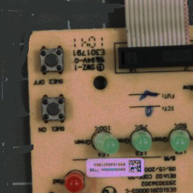
\includegraphics[width=1\textwidth]{images/guided/resize_circuit.png}
    \end{subfigure}
    \hfill
    \begin{subfigure}[t]{0.19\textwidth}
        \centering
        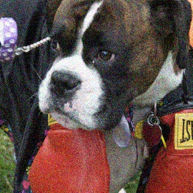
\includegraphics[width=1\textwidth]{images/guided/resize_dog.png}
    \end{subfigure}
    \hfill
    \begin{subfigure}[t]{0.19\textwidth}
        \centering
        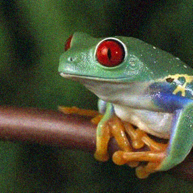
\includegraphics[width=1\textwidth]{images/guided/resize_frog.png}
    \end{subfigure}
    \hfill
    \begin{subfigure}[t]{0.19\textwidth}
        \centering
        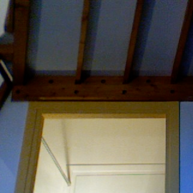
\includegraphics[width=1\textwidth]{images/guided/resize_room.png}
    \end{subfigure}
    \hfill
    \begin{subfigure}[t]{0.19\textwidth}
        \centering
        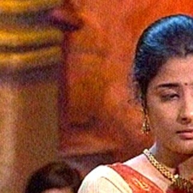
\includegraphics[width=1\textwidth]{images/guided/resize_singer.png}
    \end{subfigure}
    \hfill
    \begin{subfigure}[t]{0.19\textwidth}
        \centering
        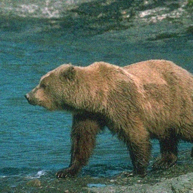
\includegraphics[width=1\textwidth]{images/guided/resize_bears.png}
    \end{subfigure}
    \hfill
    \begin{subfigure}[t]{0.19\textwidth}
        \centering
        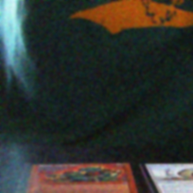
\includegraphics[width=1\textwidth]{images/guided/resize_cards.png}
    \end{subfigure}
    \hfill
    \begin{subfigure}[t]{0.19\textwidth}
        \centering
        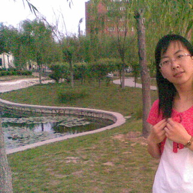
\includegraphics[width=1\textwidth]{images/guided/resize_girl.png}
    \end{subfigure}
    \hfill
    \begin{subfigure}[t]{0.19\textwidth}
        \centering
        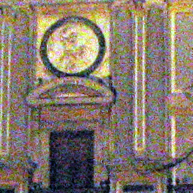
\includegraphics[width=1\textwidth]{images/guided/resize_palace.png}
    \end{subfigure}
    \hfill
    \begin{subfigure}[t]{0.19\textwidth}
        \centering
        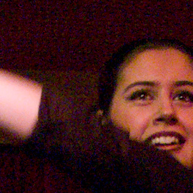
\includegraphics[width=1\textwidth]{images/guided/resize_woman.png}
    \end{subfigure}
    \caption{Some samples cropped from real noisy images of Dataset 1 \cite{ncwebsite}.}
    \label{fig3-3}
\end{figure}

\begin{figure}
    \centering
    \begin{subfigure}[t]{0.19\textwidth}
        \centering
        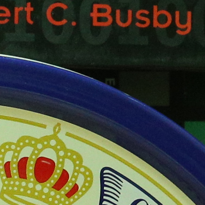
\includegraphics[width=1\textwidth]{images/mcwnnm/resize_5dmark3_iso3200_1_real.png}
    \end{subfigure}
    \hfill
    \begin{subfigure}[t]{0.19\textwidth}
        \centering
        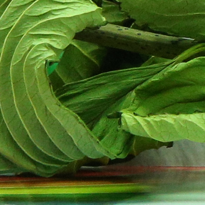
\includegraphics[width=1\textwidth]{images/mcwnnm/resize_5dmark3_iso3200_2_real.png}
    \end{subfigure}
    \hfill
    \begin{subfigure}[t]{0.19\textwidth}
        \centering
        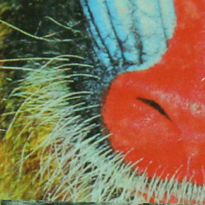
\includegraphics[width=1\textwidth]{images/mcwnnm/resize_5dmark3_iso3200_3_real.png}
    \end{subfigure}
    \hfill
    \begin{subfigure}[t]{0.19\textwidth}
        \centering
        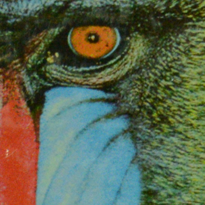
\includegraphics[width=1\textwidth]{images/mcwnnm/resize_d600_iso3200_1_real.png}
    \end{subfigure}
    \hfill
    \begin{subfigure}[t]{0.19\textwidth}
        \centering
        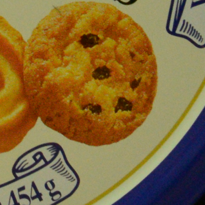
\includegraphics[width=1\textwidth]{images/mcwnnm/resize_d600_iso3200_2_real.png}
    \end{subfigure}
\hfill
    \begin{subfigure}[t]{0.19\textwidth}
        \centering
        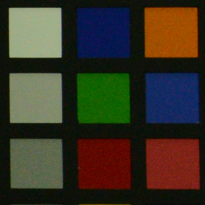
\includegraphics[width=1\textwidth]{images/mcwnnm/resize_d600_iso3200_3_real.png}
    \end{subfigure}
    \hfill
    \begin{subfigure}[t]{0.19\textwidth}
        \centering
        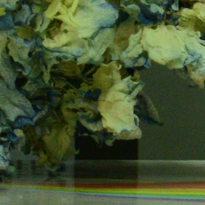
\includegraphics[width=1\textwidth]{images/mcwnnm/resize_d800_iso1600_1_real.png}
    \end{subfigure}
    \hfill
    \begin{subfigure}[t]{0.19\textwidth}
        \centering
        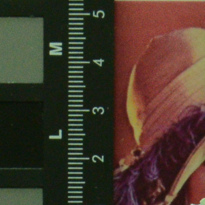
\includegraphics[width=1\textwidth]{images/mcwnnm/resize_d800_iso1600_2_real.png}
    \end{subfigure}
    \hfill
    \begin{subfigure}[t]{0.19\textwidth}
        \centering
        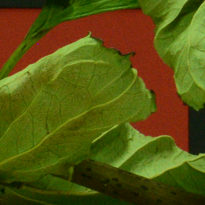
\includegraphics[width=1\textwidth]{images/mcwnnm/resize_d800_iso1600_3_real.png}
    \end{subfigure}
    \hfill
    \begin{subfigure}[t]{0.19\textwidth}
        \centering
        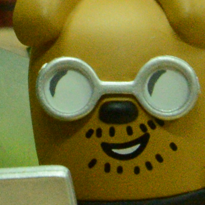
\includegraphics[width=1\textwidth]{images/mcwnnm/resize_d800_iso3200_1_real.png}
    \end{subfigure}
\hfill
    \begin{subfigure}[t]{0.19\textwidth}
        \centering
        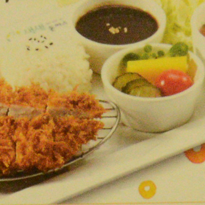
\includegraphics[width=1\textwidth]{images/mcwnnm/resize_d800_iso3200_2_real.png}
    \end{subfigure}
    \hfill
    \begin{subfigure}[t]{0.19\textwidth}
        \centering
        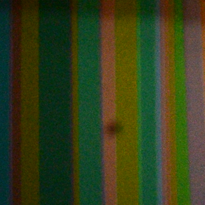
\includegraphics[width=1\textwidth]{images/mcwnnm/resize_d800_iso3200_3_real.png}
    \end{subfigure}
    \hfill
    \begin{subfigure}[t]{0.19\textwidth}
        \centering
        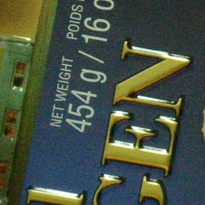
\includegraphics[width=1\textwidth]{images/mcwnnm/resize_d800_iso6400_1_real.png}
    \end{subfigure}
    \hfill
    \begin{subfigure}[t]{0.19\textwidth}
        \centering
        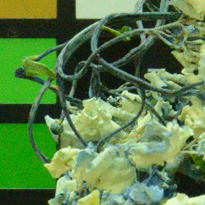
\includegraphics[width=1\textwidth]{images/mcwnnm/resize_d800_iso6400_2_real.png}
    \end{subfigure}
    \hfill
    \begin{subfigure}[t]{0.19\textwidth}
        \centering
        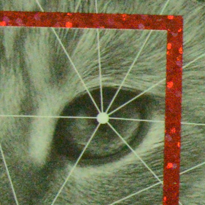
\includegraphics[width=1\textwidth]{images/mcwnnm/resize_d800_iso6400_3_real.png}
    \end{subfigure}
    \caption{The 15 cropped real noisy images used in \cite{crosschannel2016}.}
    \label{fig3-4}
\end{figure}

\begin{figure}
    \centering
    \begin{subfigure}[t]{0.19\textwidth}
        \centering
        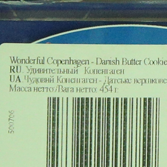
\includegraphics[width=1\textwidth]{images/guided/resize_CC_Noisy_Canon_EOS_5D_Mark3_ISO_3200_C1_52.png}
    \end{subfigure}
    \hfill
    \begin{subfigure}[t]{0.19\textwidth}
        \centering
        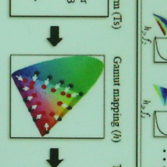
\includegraphics[width=1\textwidth]{images/guided/resize_CC_Noisy_Canon_EOS_5D_Mark3_ISO_3200_C2_44.png}
    \end{subfigure}
    \hfill
    \begin{subfigure}[t]{0.19\textwidth}
        \centering
        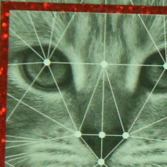
\includegraphics[width=1\textwidth]{images/guided/resize_CC_Noisy_Canon_EOS_5D_Mark3_ISO_3200_C3_26.png}
    \end{subfigure}
    \hfill
    \begin{subfigure}[t]{0.19\textwidth}
        \centering
        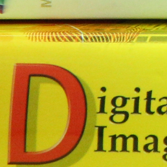
\includegraphics[width=1\textwidth]{images/guided/resize_CC_Noisy_Canon_EOS_5D_Mark3_ISO_3200_C3_73.png}
    \end{subfigure}
    \hfill
    \begin{subfigure}[t]{0.19\textwidth}
        \centering
        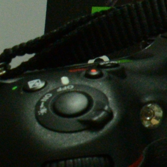
\includegraphics[width=1\textwidth]{images/guided/resize_CC_Noisy_Nikon_D600_ISO_3200_C2_67.png}
    \end{subfigure}
    \hfill
    \begin{subfigure}[t]{0.19\textwidth}
        \centering
        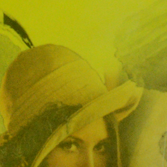
\includegraphics[width=1\textwidth]{images/guided/resize_CC_Noisy_Nikon_D800_ISO_1600_B2_80.png}
    \end{subfigure}
    \hfill
    \begin{subfigure}[t]{0.19\textwidth}
        \centering
        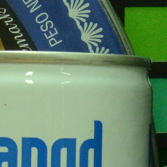
\includegraphics[width=1\textwidth]{images/guided/resize_CC_Noisy_Nikon_D800_ISO_1600_B3_82.png}
    \end{subfigure}
    \hfill
    \begin{subfigure}[t]{0.19\textwidth}
        \centering
        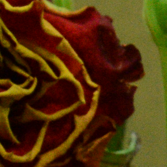
\includegraphics[width=1\textwidth]{images/guided/resize_CC_Noisy_Nikon_D800_ISO_3200_A4_51.png}
    \end{subfigure}
    \hfill
    \begin{subfigure}[t]{0.19\textwidth}
        \centering
        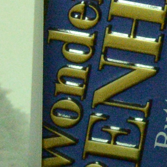
\includegraphics[width=1\textwidth]{images/guided/resize_CC_Noisy_Nikon_D800_ISO_6400_B3_95.png}
    \end{subfigure}
    \hfill
    \begin{subfigure}[t]{0.19\textwidth}
        \centering
        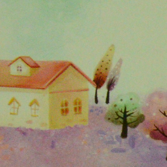
\includegraphics[width=1\textwidth]{images/guided/resize_CC_Noisy_Nikon_D800_ISO_3200_A2_80.png}
    \end{subfigure}
    \caption{Some samples cropped from real noisy images of Dataset 2 \cite{crosschannel2016}.}
    \label{fig3-5}
\end{figure}

\begin{figure}
    \centering
    \begin{subfigure}[t]{0.19\textwidth}
        \centering
        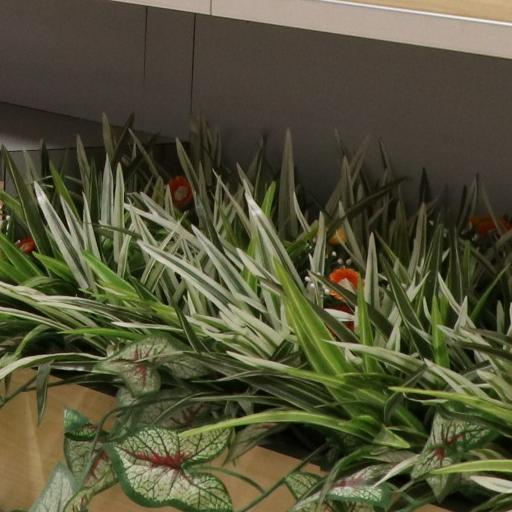
\includegraphics[width=1\textwidth]{images/guided/Canon_80D_ISO800_IMG_9916_part6.JPG}
    \end{subfigure}
    \hfill
    \begin{subfigure}[t]{0.19\textwidth}
        \centering
        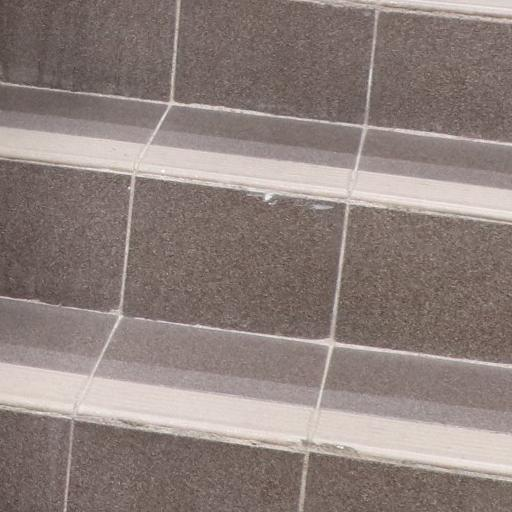
\includegraphics[width=1\textwidth]{images/guided/Canon_80D_ISO1600_IMG_1056_part2.JPG}
    \end{subfigure}
    \hfill
    \begin{subfigure}[t]{0.19\textwidth}
        \centering
        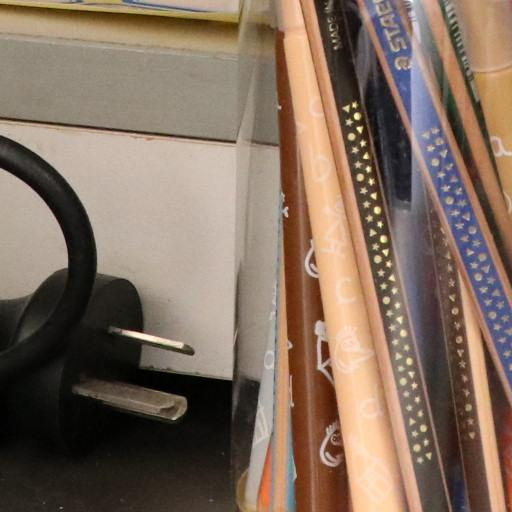
\includegraphics[width=1\textwidth]{images/guided/Canon_80D_ISO3200_IMG_8701_part8.JPG}
    \end{subfigure}
    \hfill
    \begin{subfigure}[t]{0.19\textwidth}
        \centering
        \includegraphics[width=1\textwidth]{images/guided/Canon_80D_ISO3200_IMG_8793_part10.JPG}
    \end{subfigure}
    \hfill
    \begin{subfigure}[t]{0.19\textwidth}
        \centering
        \includegraphics[width=1\textwidth]{images/guided/Canon_80D_ISO3200_IMG_9133_part4.JPG}
    \end{subfigure}
    \hfill
    \begin{subfigure}[t]{0.19\textwidth}
        \centering
        \includegraphics[width=1\textwidth]{images/guided/Canon_80D_ISO3200_IMG_9333_part6.JPG}
    \end{subfigure}
    \hfill
    \begin{subfigure}[t]{0.19\textwidth}
        \centering
        \includegraphics[width=1\textwidth]{images/guided/Canon_80D_ISO6400_IMG_0360_part2.JPG}
    \end{subfigure}
    \hfill
    \begin{subfigure}[t]{0.19\textwidth}
        \centering
        \includegraphics[width=1\textwidth]{images/guided/Canon_80D_ISO6400_IMG_0985_part5.JPG}
    \end{subfigure}
    \hfill
    \begin{subfigure}[t]{0.19\textwidth}
        \centering
        \includegraphics[width=1\textwidth]{images/guided/SONY_A7II_ISO12800_DSC02078_part1.JPG}
    \end{subfigure}
    \hfill
    \begin{subfigure}[t]{0.19\textwidth}
        \centering
        \includegraphics[width=1\textwidth]{images/guided/SONY_A7II_ISO12800_DSC02383_part8.JPG}
    \end{subfigure}
    \caption{Some samples cropped from our dataset (Dataset 3).}
    \label{fig3-6}
\end{figure}


\begin{figure}
    \centering
    \begin{subfigure}[t]{0.19\textwidth}
        \centering
        \includegraphics[width=1\textwidth]{images/guided/resize_br_Noisy_CC_Noisy_Nikon_D600_ISO_3200_C1_96.png}
		\caption{Noisy 35.89}
    \end{subfigure}
    \hfill
    \begin{subfigure}[t]{0.19\textwidth}
        \centering
        \includegraphics[width=1\textwidth]{images/guided/resize_br_Offline_CC_Noisy_Nikon_D600_ISO_3200_C1_96.png}
		\caption{External 39.05}
    \end{subfigure}
    \hfill
    \begin{subfigure}[t]{0.19\textwidth}
        \centering
        \includegraphics[width=1\textwidth]{images/guided/resize_br_Online_CC_Noisy_Nikon_D600_ISO_3200_C1_96.png}
\caption{Internal 38.75}
    \end{subfigure}
    \hfill
    \begin{subfigure}[t]{0.19\textwidth}
        \centering
        \includegraphics[width=1\textwidth]{images/guided/resize_br_Guided_CC_Noisy_Nikon_D600_ISO_3200_C1_96.png}
\caption{ Guided Internal \textbf{39.39}}
    \end{subfigure}
    \hfill
    \begin{subfigure}[t]{0.19\textwidth}
        \centering
        \includegraphics[width=1\textwidth]{images/guided/resize_br_Mean_CC_Noisy_Nikon_D600_ISO_3200_C1_96.png}
\caption{Mean Image}
    \end{subfigure}
    \caption{Denoised images and PSNR(dB) results of a region cropped from the real noisy image ``Nikon D600 ISO 3200 C1'' \cite{crosschannel2016} by different methods. The images are better to be zoomed in on screen.}
    \label{fig3-7}
\end{figure}


\begin{figure}
    \centering
    \begin{subfigure}[t]{0.19\textwidth}
        \centering
        \includegraphics[width=1\textwidth]{images/guided/resize_br_Noisy_CC_Noisy_Nikon_D600_ISO_3200_C1_94b.png}
		\caption{Noisy 33.77}
    \end{subfigure}
    \hfill
    \begin{subfigure}[t]{0.19\textwidth}
        \centering
        \includegraphics[width=1\textwidth]{images/guided/resize_br_Offline_CC_Noisy_Nikon_D600_ISO_3200_C1_94b.png}
		\caption{External 36.97}
    \end{subfigure}
    \hfill
    \begin{subfigure}[t]{0.19\textwidth}
        \centering
        \includegraphics[width=1\textwidth]{images/guided/resize_br_Online_CC_Noisy_Nikon_D600_ISO_3200_C1_94b.png}
\caption{Internal 37.40}
    \end{subfigure}
    \hfill
    \begin{subfigure}[t]{0.19\textwidth}
        \centering
        \includegraphics[width=1\textwidth]{images/guided/resize_br_Guided_CC_Noisy_Nikon_D600_ISO_3200_C1_94b.png}
\caption{ Guided Internal \textbf{38.01}}
    \end{subfigure}
    \hfill
    \begin{subfigure}[t]{0.19\textwidth}
        \centering
        \includegraphics[width=1\textwidth]{images/guided/resize_br_Mean_CC_Noisy_Nikon_D600_ISO_3200_C1_94b.png}
\caption{Mean Image}
    \end{subfigure}
    \caption{Denoised images and PSNR(dB) results of a region cropped from the real noisy image ``Nikon D600 ISO 3200 C1'' \cite{crosschannel2016} by different methods. The images are better to be zoomed in on screen.}
    \label{fig3-8}
\end{figure}


\subsection{Comparison among external, internal and guided internal priors}

To demonstrate the advantages of external prior guided internal prior learning, we perform real noisy image denoising by using external priors only (denoted by ``External''), internal priors only (denoted by ``Internal''), and the proposed guided internal priors (denoted by ``Guided Internal''), respectively.\ For the ``External'' method, we utilize the full external dictionaries (i.e., $r=108$ in Eq.\ (\ref{equ3-5})) for denoising.\ For the ``Internal'' method, the overall framework is similar to the method of \cite{ncsr}.\ A GMM model (with $K = 32$ Gaussians) is directly learned from the PGs extracted from the given noisy image without using any external data, and then the internal orthogonal dictionaries are obtained via Eq.\ (\ref{equ3-2}) to perform denoising.\ All parameters of the ``External'' and ``Internal'' methods are tuned to achieve their best performance. 

We compare the three methods on the 60 cropped images from \cite{crosschannel2016}.\ The average PSNR and run time are listed in Table \ref{tab1}.\ The best results are highlighted in bold.\ It can be seen that ``Guided Internal'' method achieves better PSNR than both ``External'' and ``Internal'' methods. In addition, the ``Internal'' method is very slow because it involves online GMM learning, while the ``Guided Internal'' method is only a little slower than the ``External'' method.\ Figs. \ref{fig3-7} and \ref{fig3-8} show the denoised images of two noisy images by the three methods.\ One can see that the  ``External'' method is good at recovering large-scale structures (see Fig. \ref{fig3-7}) while the ``Internal'' method is good at recovering fine-scale textures (see Fig. \ref{fig3-8}).\ By utilizing external priors to guide the internal prior learning, our proposed method can effectively recover both the large-scale structures and fine-scale textures. 

%------------------------------------------------------------------------------------
\begin{figure}
    \centering
    \begin{subfigure}[t]{0.19\textwidth}
        \centering
        \includegraphics[width=1\textwidth]{images/guided/resize_br_Noisy_dog.png}
		\caption{Noisy}
    \end{subfigure}
    \hfill
    \begin{subfigure}[t]{0.19\textwidth}
        \centering
        \includegraphics[width=1\textwidth]{images/guided/resize_br_BM3DPoisson_dog.png}
		\caption{GAT-BM3D}
    \end{subfigure}
    \hfill
    \begin{subfigure}[t]{0.19\textwidth}
        \centering
        \includegraphics[width=1\textwidth]{images/guided/resize_br_BM3D_dog.png}
\caption{CBM3D}
    \end{subfigure}
    \hfill
    \begin{subfigure}[t]{0.19\textwidth}
        \centering
        \includegraphics[width=1\textwidth]{images/guided/resize_br_WNNM_dog.png}
\caption{WNNM}
    \end{subfigure}
    \hfill
    \begin{subfigure}[t]{0.19\textwidth}
        \centering
        \includegraphics[width=1\textwidth]{images/guided/resize_br_CSF_dog.png}
\caption{CSF}
    \end{subfigure}
\hfill
    \begin{subfigure}[t]{0.19\textwidth}
        \centering
        \includegraphics[width=1\textwidth]{images/guided/resize_br_TRD_dog.png}
		\caption{TNRD}
    \end{subfigure}
    \hfill
    \begin{subfigure}[t]{0.19\textwidth}
        \centering
        \includegraphics[width=1\textwidth]{images/guided/resize_br_DnCNN_dog.png}
		\caption{DnCNN}
    \end{subfigure}
    \hfill
    \begin{subfigure}[t]{0.19\textwidth}
        \centering
        \includegraphics[width=1\textwidth]{images/guided/resize_br_NI_dog.png}
\caption{NI}
    \end{subfigure}
    \hfill
    \begin{subfigure}[t]{0.19\textwidth}
        \centering
        \includegraphics[width=1\textwidth]{images/guided/resize_br_NC_dog.png}
\caption{NC}
    \end{subfigure}
    \hfill
    \begin{subfigure}[t]{0.19\textwidth}
        \centering
        \includegraphics[width=1\textwidth]{images/guided/resize_br_Guided_dog.png}
\caption{Ours}
    \end{subfigure}
    \caption{Denoised images of the real noisy image ``Dog'' \cite{ncwebsite} by different methods. The images are better to be zoomed in on screen.}
    \label{fig3-9}
\end{figure}

\begin{figure}
    \centering
    \begin{subfigure}[t]{0.19\textwidth}
        \centering
        \includegraphics[width=1\textwidth]{images/guided/nc/resize_br_Noisy_frog.png}
		\caption{Noisy}
    \end{subfigure}
    \hfill
    \begin{subfigure}[t]{0.19\textwidth}
        \centering
        \includegraphics[width=1\textwidth]{images/guided/nc/resize_br_BM3DPoisson_frog.png}
		\caption{GAT-BM3D}
    \end{subfigure}
    \hfill
    \begin{subfigure}[t]{0.19\textwidth}
        \centering
        \includegraphics[width=1\textwidth]{images/guided/nc/resize_br_CBM3D_frog.png}
\caption{CBM3D}
    \end{subfigure}
    \hfill
    \begin{subfigure}[t]{0.19\textwidth}
        \centering
        \includegraphics[width=1\textwidth]{images/guided/nc/resize_br_WNNM_frog.png}
\caption{WNNM}
    \end{subfigure}
    \hfill
    \begin{subfigure}[t]{0.19\textwidth}
        \centering
        \includegraphics[width=1\textwidth]{images/guided/nc/resize_br_CSF_frog.png}
\caption{CSF}
    \end{subfigure}
\hfill
    \begin{subfigure}[t]{0.19\textwidth}
        \centering
        \includegraphics[width=1\textwidth]{images/guided/nc/resize_br_TRD_frog.png}
		\caption{TNRD}
    \end{subfigure}
    \hfill
    \begin{subfigure}[t]{0.19\textwidth}
        \centering
        \includegraphics[width=1\textwidth]{images/guided/nc/resize_br_DnCNN_frog.png}
		\caption{DnCNN}
    \end{subfigure}
    \hfill
    \begin{subfigure}[t]{0.19\textwidth}
        \centering
        \includegraphics[width=1\textwidth]{images/guided/nc/resize_br_NI_frog.png}
\caption{NI}
    \end{subfigure}
    \hfill
    \begin{subfigure}[t]{0.19\textwidth}
        \centering
        \includegraphics[width=1\textwidth]{images/guided/nc/resize_br_NC_frog.png}
\caption{NC}
    \end{subfigure}
    \hfill
    \begin{subfigure}[t]{0.19\textwidth}
        \centering
        \includegraphics[width=1\textwidth]{images/guided/nc/resize_br_Guided_frog.png}
\caption{Ours}
    \end{subfigure}
    \caption{Denoised images of the real noisy image ``Frog'' \cite{ncwebsite} by different methods. The images are better to be zoomed in on screen.}
    \label{fig3-10}
\end{figure}

\begin{figure}
    \centering
    \begin{subfigure}[t]{0.19\textwidth}
        \centering
        \includegraphics[width=1\textwidth]{images/guided/nc/resize_br_Noisy_circuit.png}
		\caption{Noisy}
    \end{subfigure}
    \hfill
    \begin{subfigure}[t]{0.19\textwidth}
        \centering
        \includegraphics[width=1\textwidth]{images/guided/nc/resize_br_BM3DPoisson_circuit.png}
		\caption{GAT-BM3D}
    \end{subfigure}
    \hfill
    \begin{subfigure}[t]{0.19\textwidth}
        \centering
        \includegraphics[width=1\textwidth]{images/guided/nc/resize_br_CBM3D_circuit.png}
\caption{CBM3D}
    \end{subfigure}
    \hfill
    \begin{subfigure}[t]{0.19\textwidth}
        \centering
        \includegraphics[width=1\textwidth]{images/guided/nc/resize_br_WNNM_circuit.png}
\caption{WNNM}
    \end{subfigure}
    \hfill
    \begin{subfigure}[t]{0.19\textwidth}
        \centering
        \includegraphics[width=1\textwidth]{images/guided/nc/resize_br_CSF_circuit.png}
\caption{CSF}
    \end{subfigure}
\hfill
    \begin{subfigure}[t]{0.19\textwidth}
        \centering
        \includegraphics[width=1\textwidth]{images/guided/nc/resize_br_TRD_circuit.png}
		\caption{TNRD}
    \end{subfigure}
    \hfill
    \begin{subfigure}[t]{0.19\textwidth}
        \centering
        \includegraphics[width=1\textwidth]{images/guided/nc/resize_br_DnCNN_circuit.png}
		\caption{DnCNN}
    \end{subfigure}
    \hfill
    \begin{subfigure}[t]{0.19\textwidth}
        \centering
        \includegraphics[width=1\textwidth]{images/guided/nc/resize_br_NI_circuit.png}
\caption{NI}
    \end{subfigure}
    \hfill
    \begin{subfigure}[t]{0.19\textwidth}
        \centering
        \includegraphics[width=1\textwidth]{images/guided/nc/resize_br_NC_circuit.png}
\caption{NC}
    \end{subfigure}
    \hfill
    \begin{subfigure}[t]{0.19\textwidth}
        \centering
        \includegraphics[width=1\textwidth]{images/guided/nc/resize_br_Guided_circuit.png}
\caption{Ours}
    \end{subfigure}
    \caption{Denoised images of the real noisy image ``Circuit'' \cite{ncwebsite} by different methods. The images are better to be zoomed in on screen.}
    \label{fig3-11}
\end{figure}

\subsection{Comparison with State-of-the-Art Denoising Methods}

\textbf{Comparison methods}.
We compare the proposed method with state-of-the-art image denoising methods, including GAT-BM3D \cite{makitalo2013optimal}, CBM3D \cite{cbm3d}, WNNM \cite{wnnm}, MLP \cite{mlp}, DnCNN \cite{dncnn}, CSF \cite{csf}, TNRD \cite{tnrd}, Noise Clinic (NC) \cite{noiseclinic,ncwebsite}, Cross-Channel (CC) \cite{crosschannel2016}, and Neat Image (NI) \cite{neatimage}.\ Among these methods, GAT-BM3D \cite{makitalo2013optimal} is a state-of-the-art Poisson noise reduction method.\ The method CBM3D \cite{cbm3d} is a state-of-the-art method for color image denoising and the noise on color images is assumed to be additive white Gaussian.\ The methods of WNNM, MLP, DnCNN, CSF, and TNRD are state-of-the-art Gaussian noise removal methods for grayscale images, and we apply them to each channel of color images for denoising. NC is a blind image denoising method, and NI is a set of commercial software for image denoising, which has been embedded into Photoshop and Corel PaintShop. The code of CC is not released but its results on the 15 cropped images are available at \cite{crosschannel2016}. Therefore, we only compare with it on the 15 cropped images in dataset 2 from \cite{crosschannel2016}. 

\textbf{Noise level of comparison methods.} 
For the CBM3D method, the standard deviation of noise on color images should be given as a parameter.\ For methods of WNNM, MLP, CSF, and TNRD, the noise level in each color channel should be input. For the DnCNN method, it is trained to deal with noise in a range of levels $0\sim55$.\ We retrain the models of discriminative denoising methods MLP, CSF, and TNRD (using the released codes by the authors) at different noise levels from $\sigma=5$ to $\sigma=50$ with a gap of $5$.\ The denoising is performed by processing each channel with the model trained at the same (or nearest) noise level.\ The noise levels ($\sigma_{r}, \sigma_{g}, \sigma_{b}$) in R, G ,B channels are assumed to be Gaussian and can be estimated via some noise estimation methods \cite{noiselevel,Chen2015ICCV}.\ In this work, we employ the method \cite{Chen2015ICCV} to estimate the noise level for each color channel.

\begin{table}\vspace{-4mm}
\caption{Average PSNR (dB) and Run Time (seconds) of the ``External'', ``Internal'', and ``Guided Internal'' methods on 60 real noisy images (of size $500\times500\times3$) cropped from \cite{crosschannel2016}.}
\vspace{-4mm}
\label{tab3-1}
\begin{center}
\renewcommand\arraystretch{1}
\begin{tabular}{|c||c|c|c|c|}
\hline
 & \small\textbf{Noisy} &\small \textbf{External} & \small\textbf{Internal} & \small\textbf{Guided Internal}  
\\
\hline
PSNR & 34.51 & 38.21 & 38.07 & \textbf{38.75} 
\\
\hline
Time & | &  \textbf{21.19}  & 312.67 & 22.26
\\
\hline
\end{tabular}
\end{center}
\vspace{-3mm}
\end{table}

\textbf{Results on dataset 1.}
Since there is no ``ground truth'' for the real noisy images in  dataset 1 \cite{ncwebsite}, we only compare the visual quality of the denoised images by different methods. (Note that method CC \cite{crosschannel2016} is not compared since its code is not available. The result of MLP is not shown here due to the limit of space.) Fig. \ref{fig3-9} show the denoised images of ``Dog''. It can be seen that CBM3D and WNNM tend to over-smooth much the image while remaining some noise caused color artifacts.\ DnCNN and TNRD are likely to remain many noise-caused color artifacts across the whole image. These results demonstrate that the methods designed with Gaussian noise model are not effective for real noise removal.\ Though NC and NI methods are specifically developed for real noisy images, their performance on noise removal is not very satisfactory.\ In comparison, our proposed method recovers much better the structures and textures (such as the eye area in ``Dog'') than the other competing methods.\ More visual comparisons can be found in Figures \ref{fig3-10} and \ref{fig3-11}.


\begin{table}\vspace{-4mm}
\scriptsize
\begin{adjustwidth}{-2cm}{}
\caption{PSNR(dB) results of different methods on 15 cropped real noisy images used in \cite{crosschannel2016}.}
\vspace{-4mm}
\label{tab3-2}
\begin{center}
\renewcommand\arraystretch{1}
\begin{tabular}{|c||c|c|c|c|c|c|c|c|c|c|c|}
\hline
Camera Settings
&\textbf{GAT-BM3D}
&\textbf{CBM3D}
&\textbf{WNNM}
&\textbf{MLP}
&\textbf{CSF}
&\textbf{TNRD}
&\textbf{DnCNN}
& \textbf{NI}
&\textbf{NC}
&\textbf{CC} 
&\textbf{Ours} 
\\
\hline
\multirow{3}{*}{\small{Canon 5D Mark III}} 
& 31.23 & 39.76 & 37.51 & 39.00 & 35.68 & 39.51 & 37.26 & 37.68 & 38.76 & 38.37 & \textbf{40.50}
\\ 
\cdashline{2-12} 
\multirow{3}{*}{ISO = 3200}   
& 30.55 & 36.40 & 33.86 & 36.34 & 34.03 & 36.47 & 34.13 & 34.87 & 35.69 & 35.37 & \textbf{37.05}
\\ 
\cdashline{2-12}    
& 27.74 & 36.37 & 31.43 & 36.33 & 32.63 & \textbf{36.45} & 34.09 & 34.77 & 35.54 & 34.91 & 36.11 
\\
\hline
\multirow{3}{*}{Nikon D600} 
& 28.55 & 34.18 & 33.46 & 34.70 & 31.78 & 34.79 & 33.62 & 34.12 & \textbf{35.57} & 34.98 & 34.88
\\ 
\cdashline{2-12} 
\multirow{3}{*}{ISO = 3200}   
& 32.01 & 35.07 & 36.09 & 36.20 & 35.16 & 36.37 & 34.48 & 35.36 & \textbf{36.70} & 35.95 & 36.31
\\ 
\cdashline{2-12}    
& 39.78 & 37.13 & 39.86 & 39.33 & 39.98 & 39.49 & 35.41 & 38.68 & 39.28 & \textbf{41.15} & 39.23
\\
\hline
\multirow{3}{*}{Nikon D800} 
& 32.24 & 36.81 & 36.35 & 37.95 & 34.84 & 38.11 & 35.79 & 37.34 & 38.01 & 37.99 & \textbf{38.40}
\\ 
\cdashline{2-12} 
\multirow{3}{*}{ISO = 1600}   
& 33.86 & 37.76 & 39.99 & 40.23 & 38.42 & 40.52 & 36.08 & 38.57 & 39.05 & 40.36 & \textbf{40.92}
\\ 
\cdashline{2-12}    
& 33.90 & 37.51 & 37.15 & 37.94 & 35.79 & 38.17 & 35.48 & 37.87 & 38.20 & 38.30 & \textbf{38.97}
\\
\hline
\multirow{3}{*}{Nikon D800} 
& 36.49 & 35.05 & 38.60 & 37.55 & 38.36 & 37.69 & 34.08 & 36.95 & 38.07 & \textbf{39.01} & 38.66
\\ 
\cdashline{2-12} 
\multirow{3}{*}{ISO = 3200}   
& 32.91 & 34.07 & 36.04 & 35.91 & 35.53 & 35.90 & 33.70 & 35.09 & 35.72 & 36.75 & \textbf{37.07}
\\ 
\cdashline{2-12}    
& \textbf{40.20} & 34.42 & 39.73 & 38.15 & 40.05 & 38.21 & 33.31 & 36.91 & 36.76 & 39.06 & 38.52
\\ 
\hline
\multirow{3}{*}{Nikon D800} 
& 29.84 & 31.13 & 33.29 & 32.69 & 34.08 & 32.81 & 29.83 & 31.28 & 33.49 & \textbf{34.61} & 33.76
\\ 
\cdashline{2-12} 
\multirow{3}{*}{ISO = 6400}   
& 27.94 & 31.22 & 31.16 & 32.33 & 32.13 & 32.33 & 30.55 & 31.38 & 32.79 & 33.21 & \textbf{33.43}
\\ 
\cdashline{2-12}    
& 29.15 & 30.97 & 31.98 & 32.29 & 31.52 & 32.29 & 30.09 & 31.40 & 32.86 & 33.22 & \textbf{33.58}
\\
\hline
Average
& 32.43 & 35.19 & 35.77 & 36.46 & 35.33 & 36.61 & 33.86 & 35.49 & 36.43 & 36.88 & \textbf{37.15}
\\
\hline
\end{tabular}
\end{center}
\vspace{-3mm}
\end{adjustwidth}
\end{table}


In this section, we provide more comparisons of the proposed method with the state-of-the-art denoising methods on the 15 cropped real noisy images used in \cite{crosschannel2016}.\ In this dataset, each scene was shot 500 times under the same camera and camera setting.\ The mean image of the 500 shots is roughly taken as the ``ground truth'', with which the PSNR and SSIM \cite{ssim} can be computed.\  The average SSIM results of GAT-BM3D \cite{makitalo2013optimal}, CBM3D \cite{bm3d}, WNNM \cite{wnnm}, MLP \cite{mlp}, CSF \cite{csf}, TNRD \cite{tnrd}, DnCNN \cite{dncnn}, NI \cite{neatimage}, NC \cite{noiseclinic,ncwebsite}, CC \cite{crosschannel2016}, and the proposed method are listed in Table \ref{tab3-1}. As can be seen from Figures \ref{fig3-3}-\ref{fig3-5}, our proposed method achieves better performance than the the competing methods.

\begin{table}[htpb]
\begin{adjustwidth}{-3cm}{}
\caption{SSIM \cite{ssim} results of different methods on 15 cropped real noisy images used in \cite{crosschannel2016}.}
\vspace{-3mm}
\label{tab3-3}
\scriptsize
\begin{center}
\renewcommand\arraystretch{1}
\begin{tabular}{|c||c|c|c|c|c|c|c|c|c|c|c|}
\hline
Camera Settings
&
\textbf{GAT-BM3D}
&
\textbf{CBM3D}
&
\textbf{WNNM}
&
\textbf{MLP}
&
\textbf{CSF}
&
\textbf{TNRD}
&
\textbf{DnCNN}
&
\textbf{NI}
& 
\textbf{NC}
& 
\textbf{CC} 
&
\textbf{Ours} 
\\
\hline
\multirow{3}{*}{\small{Canon 5D Mark III}} 
& 0.9126 & 0.9778 & 0.9673 & 0.9695 & 0.9434 & 0.9742 & 0.9389 & 0.9600 & 0.9689 & 0.9678 & \textbf{0.9813}
\\ 
\cdashline{2-11} 
\multirow{3}{*}{ISO = 3200}   
& 0.8427 & 0.9552 & 0.9210 & 0.9458 & 0.9011 & 0.9491 & 0.8989 & 0.9308 & 0.9427 & 0.9359 & \textbf{0.9572}
\\ 
\cdashline{2-11}    
& 0.8017 & \textbf{0.9660} & 0.9110 & 0.9599 & 0.9037 & 0.9617 & 0.9182 & 0.9463 & 0.9476 & 0.9478 &  0.9643
\\
\hline
\multirow{3}{*}{Nikon D600} 
& 0.7845 & 0.9330 & 0.9281 & 0.9481 & 0.8792 & 0.9494 & 0.9123 & 0.9413 & 0.9497 & 0.9484 &  \textbf{0.9535}
\\ 
\cdashline{2-11} 
\multirow{3}{*}{ISO = 3200}   
& 0.9028 & 0.9168 & 0.9432 & 0.9469 & 0.9261 & \textbf{0.9499} & 0.8932 & 0.9251 & 0.9398 & 0.9293 &  0.9461
\\ 
\cdashline{2-11}    
& \textbf{0.9806} & 0.9313 & 0.9737 & 0.9726 & 0.9763 & 0.9742 & 0.8708 & 0.9481 & 0.9588 & 0.9799 &  0.9683
\\
\hline
\multirow{3}{*}{Nikon D800} 
& 0.8791 & 0.9339 & 0.9417 & 0.9543 & 0.9148 & 0.9572 & 0.9060 & 0.9506 & 0.9533 & 0.9575 &  \textbf{0.9620}
\\ 
\cdashline{2-11} 
\multirow{3}{*}{ISO = 1600}   
& 0.9534 & 0.9383 & 0.9748 & 0.9743 & 0.9674 & 0.9774 & 0.8943 & 0.9615 & 0.9591 & 0.9767 &  \textbf{0.9779}
\\ 
\cdashline{2-11}    
& 0.8795 & 0.9277 & 0.9311 & 0.9354 & 0.9035 & 0.9410 & 0.8735 & 0.9229 & 0.9406 & 0.9427 &  \textbf{0.9531}
\\
\hline
\multirow{3}{*}{Nikon D800} 
& 0.9526 & 0.8866 & \textbf{0.9656} & 0.9533 & 0.9654 & 0.9569 & 0.8463 & 0.9101 & 0.9466 & 0.9637 &  0.9613
\\ 
\cdashline{2-11} 
\multirow{3}{*}{ISO = 3200}   
& 0.9078 & 0.8928 & 0.9416 & 0.9381 & 0.9354 & 0.9394 & 0.8755 & 0.9194 & 0.9309 & 0.9477 &  \textbf{0.9521}
\\ 
\cdashline{2-11}    
& 0.9707 & 0.8430 & 0.9664 & 0.9548 & \textbf{0.9712} & 0.9576 & 0.7204 & 0.9001 & 0.9070 & 0.9544 &  0.9512
\\ 
\hline
\multirow{3}{*}{Nikon D800} 
& 0.8909 & 0.7952 & 0.9188 & 0.8914 & \textbf{0.9259} & 0.8966 & 0.7847 & 0.7781 & 0.9024 & 0.9206 &  0.8958
\\ 
\cdashline{2-11} 
\multirow{3}{*}{ISO = 6400}   
& 0.8328 & 0.8613 & 0.9050 & 0.9137 & 0.9127 & 0.9142 & 0.8259 & 0.8649 & 0.9141 & \textbf{0.9369} &  0.9238
\\ 
\cdashline{2-11}    
& 0.7773 & 0.8363 & 0.8818 & 0.8958 & 0.8494 & 0.8960 & 0.7936 & 0.8295 & 0.8847 & \textbf{0.9118} & 0.9089
\\
\hline
Average
& 0.8846 & 0.9063 & 0.9381 & 0.9436 & 0.9250 & 0.9463 & 0.8635 & 0.9126 & 0.9364 & 0.9481 & \textbf{0.9504}
\\
\hline
\end{tabular}
\end{center}
\end{adjustwidth}
\end{table}

\textbf{Results on dataset 2.}
As described in section 3.4.2, there is a mean image for each of the 11 scenes used in dataset 2 \cite{crosschannel2016}, and those mean images can be roughly taken as ``ground truth'' images for quantitative evaluation of denoising algorithms. We firstly perform quantitative comparison on the 15 cropped images used in \cite{crosschannel2016}. The PSNR results of GAT-BM3D, CBM3D, WNNM, MLP, CSF, TNRD, DnCNN, NC, NI and CC are listed in Table II (The results of CC are copied from the original paper \cite{crosschannel2016}). The best PSNR results of each image are highlighted in bold. One can see that on 8 out of the 15 images, our method achieves the best PSNR values. CC achieves the best PSNR on 3 of the 15 images. It should be noted that in the CC method, a specific model is trained for each camera and camera setting, while our method uses the same model for all images. On average, our proposed method has 0.27dB PSNR improvements over the second best method CC and much higher PSNR gains over other competing methods. The method GAT-BM3D does not work well on most images. This is because real world noise is much more complex than Poisson. 

Fig. \ref{fig3-12} shows the denoised images of one scene captured by Canon 5D Mark 3 at ISO = 3200. We can see that GAT-BM3D, CBM3D, WNNM, DnCNN, NC, NI and CC would either remain noise or generate artifacts, while TNRD over-smooths much the image. By using the external prior guided internal priors, our proposed method preserves edges and textures better than other methods, leading to visually pleasant outputs. More comparisons on visual quality and SSIM \cite{ssim} index can be found in the Figures \ref{fig3-13} and \ref{fig3-14}.

We then perform denoising experiments on the 60 images we cropped from \cite{crosschannel2016}. The average PSNR results are listed in Table III (CC is not compared since the code is not available). Again, our proposed method achieves much better PSNR results than the other methods. The improvements of our method over the second best method (TNRD) are 0.43dB on PSNR. Fig. \ref{fig3-15} shows the denoised images of one scene captured by Nikon D800 at ISO = 3200. We can see again that the proposed method obtain better visual quality than other competing methods. More comparisons on visual quality and SSIM can be found in the Figures \ref{fig3-16} and \ref{fig3-17}.

\textbf{Results on dataset 3.}
Similar to dataset 2 \cite{crosschannel2016}, there is a ``ground truth'' image for each of the 10 scenes used in our constructed dataset 3. We perform quantitative comparison on the 100 cropped images. The average PSNR results of competing methods are listed in Table IV. We can see that our proposed method achieves much better PSNR results than the other methods. The improvements of our method over the second best method (TNRD) is 0.16dB on PSNR. Fig. \ref{fig3-18} shows the denoised images of one scene captured by Canon 80D at ISO = 12800. We can see again that the proposed method removes the noise while maintains better details (such as the vertical black shadow area) than other competing methods. More comparisons on visual quality and SSIM can be found in the Figures \ref{fig3-19} and \ref{fig3-20}.

\textbf{Comparison on speed.}
Efficiency is an important aspect to evaluate the efficiency of algorithms. We compare the speed of all competing methods except for CC. All experiments are run under the Matlab2014b environment on a machine with Intel(R) Core(TM) i7-5930K CPU of 3.5GHz and 32GB RAM. The average running time (second) of the compared methods on the 100 real noisy images is shown in Table \ref{tab3-5}. The least average running time are highlighted in bold. One can easily see that the commercial software Neat Image (NI) is the fastest method with highly optimized code. For a $512\times512$ image, NI costs about 0.6 second. The other methods cost from 5.2 (TNRD) to 152.2 (WNNM) seconds, while the proposed method costs about 24.1 seconds. It should be noted that GAT-BM3D, CBM3D, TNRD, and NC are implemented with compiled C++ mex-function and with parallelization, while WNNM, MLP, CSF, DnCNN, and the proposed method are implemented purely in Matlab. 


\begin{figure}
    \centering
    \begin{subfigure}[t]{0.19\textwidth}
        \centering
        \includegraphics[width=1\textwidth]{images/guided/resize_br_Noisy_5dmark3_iso3200_1_real.png}
		\caption{Noisy 37.00}
    \end{subfigure}
    \hfill
    \begin{subfigure}[t]{0.19\textwidth}
        \centering
        \includegraphics[width=1\textwidth]{images/guided/resize_br_CBM3D_5dmark3_iso3200_1_real.png}
		\caption{CBM3D39.76}
    \end{subfigure}
    \hfill
    \begin{subfigure}[t]{0.19\textwidth}
        \centering
        \includegraphics[width=1\textwidth]{images/guided/resize_br_WNNM_5dmark3_iso3200_1_real.png}
\caption{WNNM 37.51}
    \end{subfigure}
    \hfill
    \begin{subfigure}[t]{0.19\textwidth}
        \centering
        \includegraphics[width=1\textwidth]{images/guided/resize_br_TRD_5dmark3_iso3200_1_real.png}
\caption{TNRD 39.51}
    \end{subfigure}
    \hfill
    \begin{subfigure}[t]{0.19\textwidth}
        \centering
        \includegraphics[width=1\textwidth]{images/guided/resize_br_DnCNN_5dmark3_iso3200_1_real.png}
\caption{DnCNN 37.26}
    \end{subfigure}
\hfill
    \begin{subfigure}[t]{0.19\textwidth}
        \centering
        \includegraphics[width=1\textwidth]{images/guided/resize_br_NI_5dmark3_iso3200_1_real.png}
		\caption{NI 37.68}
    \end{subfigure}
    \hfill
    \begin{subfigure}[t]{0.19\textwidth}
        \centering
        \includegraphics[width=1\textwidth]{images/guided/resize_br_NC_5dmark3_iso3200_1_real.png}
		\caption{NC 38.76}
    \end{subfigure}
    \hfill
    \begin{subfigure}[t]{0.19\textwidth}
        \centering
        \includegraphics[width=1\textwidth]{images/guided/resize_br_CCNoise_5dmark3_iso3200_1.png}
\caption{CC 38.37}
    \end{subfigure}
    \hfill
    \begin{subfigure}[t]{0.19\textwidth}
        \centering
        \includegraphics[width=1\textwidth]{images/guided/resize_br_Guided_5dmark3_iso3200_1.png}
\caption{Ours \textbf{40.50}}
    \end{subfigure}
    \hfill
    \begin{subfigure}[t]{0.19\textwidth}
        \centering
        \includegraphics[width=1\textwidth]{images/guided/resize_br_Mean_5dmark3_iso3200_1_real.png}
\caption{Mean Image}
    \end{subfigure}
    \caption{Denoised images and PSNR(dB) results of a region cropped from the real noisy image ``Canon 5D Mark 3 ISO 3200 1'' \cite{crosschannel2016} by different methods. The images are better to be zoomed in on screen.}
    \label{fig3-12}
\end{figure}


\begin{figure}
    \centering
    \begin{subfigure}[t]{0.19\textwidth}
        \centering
        \includegraphics[width=1\textwidth]{images/guided/cc15/resize_br_Noisy_5dmark3_iso3200_2_real.png}
		\caption{Noisy 33.88}
    \end{subfigure}
    \hfill
    \begin{subfigure}[t]{0.19\textwidth}
        \centering
        \includegraphics[width=1\textwidth]{images/guided/cc15/resize_br_CBM3D_5dmark3_iso3200_2_real.png}
		\caption{CBM3D 36.40}
    \end{subfigure}
    \hfill
    \begin{subfigure}[t]{0.19\textwidth}
        \centering
        \includegraphics[width=1\textwidth]{images/guided/cc15/resize_br_WNNM_5dmark3_iso3200_2_real.png}
\caption{WNNM 33.86}
    \end{subfigure}
    \hfill
    \begin{subfigure}[t]{0.19\textwidth}
        \centering
        \includegraphics[width=1\textwidth]{images/guided/cc15/resize_br_TRD_5dmark3_iso3200_2_real.png}
\caption{TNRD 36.47}
    \end{subfigure}
    \hfill
    \begin{subfigure}[t]{0.19\textwidth}
        \centering
        \includegraphics[width=1\textwidth]{images/guided/cc15/resize_br_DnCNN_5dmark3_iso3200_2_real.png}
\caption{DnCNN 34.13}
    \end{subfigure}
\hfill
    \begin{subfigure}[t]{0.19\textwidth}
        \centering
        \includegraphics[width=1\textwidth]{images/guided/cc15/resize_br_NI_5dmark3_iso3200_2_real.png}
		\caption{NI 34.87}
    \end{subfigure}
    \hfill
    \begin{subfigure}[t]{0.19\textwidth}
        \centering
        \includegraphics[width=1\textwidth]{images/guided/cc15/resize_br_NC_5dmark3_iso3200_2_real.png}
		\caption{NC 35.69}
    \end{subfigure}
    \hfill
    \begin{subfigure}[t]{0.19\textwidth}
        \centering
        \includegraphics[width=1\textwidth]{images/guided/cc15/resize_br_CCNoise_5dmark3_iso3200_2.png}
\caption{CC 35.37}
    \end{subfigure}
    \hfill
    \begin{subfigure}[t]{0.19\textwidth}
        \centering
        \includegraphics[width=1\textwidth]{images/guided/cc15/resize_br_Guided_5dmark3_iso3200_2_real.png}
\caption{Ours \textbf{37.05}}
    \end{subfigure}
    \hfill
    \begin{subfigure}[t]{0.19\textwidth}
        \centering
        \includegraphics[width=1\textwidth]{images/guided/cc15/resize_br_Mean_5dmark3_iso3200_2_real.png}
\caption{Mean Image}
    \end{subfigure}
    \caption{Denoised images and PSNR(dB) results of a region cropped from the real noisy image ``Canon 5D Mark 3 ISO 3200 2'' \cite{crosschannel2016} by different methods. The images are better to be zoomed in on screen.}
    \label{fig3-13}
\end{figure}

\begin{figure}
    \centering
    \begin{subfigure}[t]{0.19\textwidth}
        \centering
        \includegraphics[width=1\textwidth]{images/guided/cc15/resize_br_Noisy_d600_iso3200_2_real.png}
		\caption{Noisy 33.77}
    \end{subfigure}
    \hfill
    \begin{subfigure}[t]{0.19\textwidth}
        \centering
        \includegraphics[width=1\textwidth]{images/guided/cc15/resize_br_CBM3D_d600_iso3200_2_real.png}
		\caption{CBM3D 35.07}
    \end{subfigure}
    \hfill
    \begin{subfigure}[t]{0.19\textwidth}
        \centering
        \includegraphics[width=1\textwidth]{images/guided/cc15/resize_br_WNNM_d600_iso3200_2_real.png}
\caption{WNNM 36.09}
    \end{subfigure}
    \hfill
    \begin{subfigure}[t]{0.19\textwidth}
        \centering
        \includegraphics[width=1\textwidth]{images/guided/cc15/resize_br_TRD_d600_iso3200_2_real.png}
\caption{TNRD 36.37}
    \end{subfigure}
    \hfill
    \begin{subfigure}[t]{0.19\textwidth}
        \centering
        \includegraphics[width=1\textwidth]{images/guided/cc15/resize_br_DnCNN_d600_iso3200_2_real.png}
\caption{DnCNN 34.48}
    \end{subfigure}
\hfill
    \begin{subfigure}[t]{0.19\textwidth}
        \centering
        \includegraphics[width=1\textwidth]{images/guided/cc15/resize_br_NI_d600_iso3200_2_real.png}
		\caption{NI 35.36}
    \end{subfigure}
    \hfill
    \begin{subfigure}[t]{0.19\textwidth}
        \centering
        \includegraphics[width=1\textwidth]{images/guided/cc15/resize_br_NC_d600_iso3200_2_real.png}
		\caption{NC \textbf{36.70}}
    \end{subfigure}
    \hfill
    \begin{subfigure}[t]{0.19\textwidth}
        \centering
        \includegraphics[width=1\textwidth]{images/guided/cc15/resize_br_CCNoise_d600_iso3200_2.png}
\caption{CC 35.95}
    \end{subfigure}
    \hfill
    \begin{subfigure}[t]{0.19\textwidth}
        \centering
        \includegraphics[width=1\textwidth]{images/guided/cc15/resize_br_Guided_d600_iso3200_2_real.png}
\caption{Ours 36.31}
    \end{subfigure}
    \hfill
    \begin{subfigure}[t]{0.19\textwidth}
        \centering
        \includegraphics[width=1\textwidth]{images/guided/cc15/resize_br_Mean_d600_iso3200_2_real.png}
\caption{Mean Image}
    \end{subfigure}
    \caption{Denoised images and PSNR(dB) results of a region cropped from the real noisy image ``Nikon D600 ISO 3200 2'' \cite{crosschannel2016} by different methods. The images are better to be zoomed in on screen.}
    \label{fig3-14}
\end{figure}


\begin{table}
\begin{adjustwidth}{-1cm}{}
\scriptsize
\caption{Average PSNR(dB) results of different methods on 60 real noisy images cropped from \cite{crosschannel2016}.}
\vspace{-4mm}
\label{tab3-4}
\begin{center}
\renewcommand\arraystretch{1}
\begin{tabular}{|c||c|c|c|c|c|c|c|c|c|c|}
\hline
Methods
&\textbf{GAT-BM3D}
&\textbf{CBM3D}
&\textbf{WNNM}
&\textbf{MLP}
&\textbf{CSF} 
&\textbf{TNRD} 
&\textbf{DnCNN}
&\textbf{NI} 
&\textbf{NC} 
&\textbf{Ours} 
\\
\hline
PSNR  
& 34.33 & 36.34 & 37.67 & 38.13 & 37.40 & 38.32 & 34.99 & 36.53 & 37.57 & \textbf{38.75}
\\
\hline
\end{tabular}
\end{center}
\end{adjustwidth}
\end{table}

In this section, we provide more comparisons of the proposed method with the state-of-the-art denoising methods on the 60 real noisy images cropped from \cite{crosschannel2016}.\ In this dataset, each scene was shot 500 times under the same camera and camera setting.\ The mean image of the 500 shots is roughly taken as the ``ground truth'', with which the PSNR and SSIM can be computed.\ The average SSIM results of GAT-BM3D \cite{makitalo2013optimal}, CBM3D \cite{bm3d}, WNNM \cite{wnnm}, MLP \cite{mlp}, CSF \cite{csf}, TNRD \cite{tnrd}, DnCNN \cite{dncnn}, NI \cite{neatimage}, NC \cite{noiseclinic,ncwebsite}, and the proposed method are listed in Table \ref{tab3-4} (CC is not compared since the code of \cite{crosschannel2016} is not available).\ As can be seen from Figures \ref{fig3-6}-\ref{fig3-7}, our proposed method achieves better performance than the competing methods.

\begin{table}[htpb]
\begin{adjustwidth}{-1cm}{}
\scriptsize
\caption{Average SSIM \cite{ssim} results of different methods on 60 real noisy images cropped from \cite{crosschannel2016}.}
\label{tab3-5}
\begin{center}
\renewcommand\arraystretch{1}
\begin{tabular}{|c||c|c|c|c|c|c|c|c|c|c|}
\hline
Methods
&\textbf{GAT-BM3D}
&\textbf{CBM3D}
&\textbf{WNNM}
&\textbf{MLP}
&\textbf{CSF} 
&\textbf{TNRD} 
&\textbf{DnCNN}
&\textbf{NI} 
&\textbf{NC} 
&\textbf{Ours} 
\\
\hline
SSIM  
& 0.9331 & 0.9251 & 0.9633 & 0.9653 & 0.9598 & 0.9670 & 0.8873 & 0.9241 & 0.9514 & \textbf{0.9691}
\\
\hline
\end{tabular}
\end{center}
\end{adjustwidth}
\end{table}




\begin{table}
\begin{adjustwidth}{-2cm}{}
\scriptsize
\caption{Average PSNR(dB) results of different methods on 100 real noisy images cropped from our new dataset.}
\vspace{-4mm}
\label{tab3-6}
\begin{center}
\renewcommand\arraystretch{1}
\begin{tabular}{|c||c|c|c|c|c|c|c|c|c|c|}
\hline
Methods
&\textbf{GAT-BM3D}
&\textbf{CBM3D}
&\textbf{WNNM}
&\textbf{MLP}
&\textbf{CSF} 
&\textbf{TNRD} 
&\textbf{DnCNN}
&\textbf{NI} 
&\textbf{NC} 
&\textbf{Ours} 
\\
\hline
PSNR  
& 33.54 & 37.14 & 35.18 & 37.34 & 37.07 & 37.48 & 34.74 & 35.70 & 36.76 & \textbf{37.64}
\\
\hline
\end{tabular}
\end{center}
\end{adjustwidth}
\end{table}

In this section, we provide more comparisons of the proposed method with the state-of-the-art denoising methods on the 100 real noisy images cropped from the new dataset we constructed.\ In this dataset, each scene was shot 500 times under the same camera and camera setting.\ The mean image of the 500 shots is roughly taken as the ``ground truth'', with which the PSNR and SSIM can be computed.\ The average  SSIM results of GAT-BM3D \cite{makitalo2013optimal}, CBM3D \cite{bm3d}, WNNM \cite{wnnm}, MLP \cite{mlp}, CSF \cite{csf}, TNRD \cite{tnrd}, DnCNN \cite{dncnn}, NI \cite{neatimage}, NC \cite{noiseclinic,ncwebsite}, and the proposed method are listed in Table \ref{tab3-7} (CC is not compared since the code of \cite{crosschannel2016} is not available).\ As can be seen from Figure \ref{fig3-12}, our proposed method achieves better performance than the competing methods.


\begin{table}[htpb]
\begin{adjustwidth}{-1cm}{}
\scriptsize
\caption{Average SSIM \cite{ssim} results of different methods on 100 real noisy images cropped from our new dataset.}
\label{tab3-7}
\begin{center}
\renewcommand\arraystretch{1}
\begin{tabular}{|c||c|c|c|c|c|c|c|c|c|c|}
\hline
Methods
&\textbf{GAT-BM3D}
&\textbf{CBM3D}
&\textbf{WNNM}
&\textbf{MLP}
&\textbf{CSF} 
&\textbf{TNRD} 
&\textbf{DnCNN}
&\textbf{NI} 
&\textbf{NC} 
&\textbf{Ours} 
\\
\hline
SSIM  
& 0.8881 & 0.9494 & 0.9290 & 0.9453 & 0.9398 & 0.9486 & 0.8852 & 0.9190 & 0.9356 & \textbf{0.9529}
\\
\hline
\end{tabular}
\end{center}
\end{adjustwidth}
\end{table}



\begin{table}\vspace{-4mm}
\begin{adjustwidth}{-1cm}{}
\scriptsize
\caption{Average Speed (sec.) results of different methods on 100 real noisy images cropped from our new dataset.}
\vspace{-4mm}
\label{tab3-8}
\begin{center}
\renewcommand\arraystretch{1}
\begin{tabular}{|c||c|c|c|c|c|c|c|c|c|c|}
\hline
Methods
&\textbf{GAT-BM3D}
&\textbf{CBM3D}
&\textbf{WNNM}
&\textbf{MLP}
&\textbf{CSF} 
&\textbf{TNRD} 
&\textbf{DnCNN}
&\textbf{NI} 
&\textbf{NC} 
&\textbf{Ours} 
\\
\hline
Time  
& 11.1 & 6.9 & 152.2 & 17.1 & 19.5 & 5.2 & 79.5 & \textbf{0.6} & 15.6 & 24.1
\\
\hline
\end{tabular}
\end{center}
\end{adjustwidth}
\end{table}


%------------------------------------------------------------------------------------
\begin{figure}
    \centering
    \begin{subfigure}[t]{0.19\textwidth}
        \centering
        \includegraphics[width=1\textwidth]{images/guided/resize_br_Noisy_CC_Noisy_Nikon_D800_ISO_3200_A3_96.png}
		\caption{Noisy 33.60}
    \end{subfigure}
    \hfill
    \begin{subfigure}[t]{0.19\textwidth}
        \centering
        \includegraphics[width=1\textwidth]{images/guided/resize_br_CBM3D_CC_Noisy_Nikon_D800_ISO_3200_A3_96.png}
		\caption{CBM3D35.23}
    \end{subfigure}
    \hfill
    \begin{subfigure}[t]{0.19\textwidth}
        \centering
        \includegraphics[width=1\textwidth]{images/guided/resize_br_WNNM_CC_Noisy_Nikon_D800_ISO_3200_A3_96.png}
\caption{WNNM 36.50}
    \end{subfigure}
    \hfill
    \begin{subfigure}[t]{0.19\textwidth}
        \centering
        \includegraphics[width=1\textwidth]{images/guided/resize_br_CSF_CC_Noisy_Nikon_D800_ISO_3200_A3_96.png}
\caption{CSF 36.21}
    \end{subfigure}
    \hfill
    \begin{subfigure}[t]{0.19\textwidth}
        \centering
        \includegraphics[width=1\textwidth]{images/guided/resize_br_TRD_CC_Noisy_Nikon_D800_ISO_3200_A3_96.png}
\caption{TNRD 37.10}
    \end{subfigure}
\hfill
    \begin{subfigure}[t]{0.19\textwidth}
        \centering
        \includegraphics[width=1\textwidth]{images/guided/resize_br_DnCNN_CC_Noisy_Nikon_D800_ISO_3200_A3_96.png}
		\caption{DnCNN 34.43}
    \end{subfigure}
    \hfill
    \begin{subfigure}[t]{0.19\textwidth}
        \centering
        \includegraphics[width=1\textwidth]{images/guided/resize_br_NI_CC_Noisy_Nikon_D800_ISO_3200_A3_96.png}
		\caption{NI 35.02}
    \end{subfigure}
    \hfill
    \begin{subfigure}[t]{0.19\textwidth}
        \centering
        \includegraphics[width=1\textwidth]{images/guided/resize_br_NC_CC_Noisy_Nikon_D800_ISO_3200_A3_96.png}
\caption{NC 36.07}
    \end{subfigure}
    \hfill
    \begin{subfigure}[t]{0.19\textwidth}
        \centering
        \includegraphics[width=1\textwidth]{images/guided/resize_br_Guided_CC_Noisy_Nikon_D800_ISO_3200_A3_96.png}
\caption{Ours \textbf{37.50}}
    \end{subfigure}
    \hfill
    \begin{subfigure}[t]{0.19\textwidth}
        \centering
        \includegraphics[width=1\textwidth]{images/guided/resize_br_Mean_CC_Noisy_Nikon_D800_ISO_3200_A3_96.png}
\caption{Mean Image}
    \end{subfigure}
    \caption{Denoised images and PSNR(dB) results of a region cropped from the real noisy image ``Nikon D800 ISO 3200 A3'' \cite{crosschannel2016} by different methods. The images are better to be zoomed in on screen.}
    \label{fig3-15}
\end{figure}

\begin{figure}
    \centering
    \begin{subfigure}[t]{0.19\textwidth}
        \centering
        \includegraphics[width=1\textwidth]{images/guided/cc60/resize_br_Noisy_CC_Noisy_Nikon_D800_ISO_1600_B2_109.png}
		\caption{Noisy 35.21}
    \end{subfigure}
    \hfill
    \begin{subfigure}[t]{0.19\textwidth}
        \centering
        \includegraphics[width=1\textwidth]{images/guided/cc60/resize_br_CBM3D_CC_Noisy_Nikon_D800_ISO_1600_B2_109.png}
		\caption{CBM3D 37.71}
    \end{subfigure}
    \hfill
    \begin{subfigure}[t]{0.19\textwidth}
        \centering
        \includegraphics[width=1\textwidth]{images/guided/cc60/resize_br_WNNM_CC_Noisy_Nikon_D800_ISO_1600_B2_109.png}
\caption{WNNM 39.61}
    \end{subfigure}
    \hfill
    \begin{subfigure}[t]{0.19\textwidth}
        \centering
        \includegraphics[width=1\textwidth]{images/guided/cc60/resize_br_CSF_CC_Noisy_Nikon_D800_ISO_1600_B2_109.png}
\caption{CSF 38.14}
    \end{subfigure}
    \hfill
    \begin{subfigure}[t]{0.19\textwidth}
        \centering
        \includegraphics[width=1\textwidth]{images/guided/cc60/resize_br_TRD_CC_Noisy_Nikon_D800_ISO_1600_B2_109.png}
\caption{TNRD 39.04}
    \end{subfigure}
\hfill
    \begin{subfigure}[t]{0.19\textwidth}
        \centering
        \includegraphics[width=1\textwidth]{images/guided/cc60/resize_br_DnCNN_CC_Noisy_Nikon_D800_ISO_1600_B2_109.png}
		\caption{DnCNN 35.68}
    \end{subfigure}
    \hfill
    \begin{subfigure}[t]{0.19\textwidth}
        \centering
        \includegraphics[width=1\textwidth]{images/guided/cc60/resize_br_NI_CC_Noisy_Nikon_D800_ISO_1600_B2_109.png}
		\caption{NI 37.41}
    \end{subfigure}
    \hfill
    \begin{subfigure}[t]{0.19\textwidth}
        \centering
        \includegraphics[width=1\textwidth]{images/guided/cc60/resize_br_NC_CC_Noisy_Nikon_D800_ISO_1600_B2_109.png}
\caption{NC 39.53}
    \end{subfigure}
    \hfill
    \begin{subfigure}[t]{0.19\textwidth}
        \centering
        \includegraphics[width=1\textwidth]{images/guided/cc60/resize_br_Guided_CC_Noisy_Nikon_D800_ISO_1600_B2_109.png}
\caption{Ours \textbf{39.96}}
    \end{subfigure}
    \hfill
    \begin{subfigure}[t]{0.19\textwidth}
        \centering
        \includegraphics[width=1\textwidth]{images/guided/cc60/resize_br_Mean_CC_Noisy_Nikon_D800_ISO_1600_B2_109.png}
\caption{Mean Image}
    \end{subfigure}
    \caption{Denoised images and PSNR(dB) results of a region cropped from the real noisy image ``Nikon D800 ISO 1600 B2'' \cite{crosschannel2016} by different methods. The images are better to be zoomed in on screen.}
    \label{fig3-16}
\end{figure}


\begin{figure}
    \centering
    \begin{subfigure}[t]{0.19\textwidth}
        \centering
        \includegraphics[width=1\textwidth]{images/guided/cc60/resize_br_Noisy_CC_Noisy_Nikon_D800_ISO_3200_A1_111.png}
		\caption{Noisy 34.02}
    \end{subfigure}
    \hfill
    \begin{subfigure}[t]{0.19\textwidth}
        \centering
        \includegraphics[width=1\textwidth]{images/guided/cc60/resize_br_CBM3D_CC_Noisy_Nikon_D800_ISO_3200_A1_111.png}
		\caption{CBM3D 35.45}
    \end{subfigure}
    \hfill
    \begin{subfigure}[t]{0.19\textwidth}
        \centering
        \includegraphics[width=1\textwidth]{images/guided/cc60/resize_br_WNNM_CC_Noisy_Nikon_D800_ISO_3200_A1_111.png}
\caption{WNNM 34.60}
    \end{subfigure}
    \hfill
    \begin{subfigure}[t]{0.19\textwidth}
        \centering
        \includegraphics[width=1\textwidth]{images/guided/cc60/resize_br_CSF_CC_Noisy_Nikon_D800_ISO_3200_A1_111.png}
\caption{CSF 32.94}
    \end{subfigure}
    \hfill
    \begin{subfigure}[t]{0.19\textwidth}
        \centering
        \includegraphics[width=1\textwidth]{images/guided/cc60/resize_br_TRD_CC_Noisy_Nikon_D800_ISO_3200_A1_111.png}
\caption{TNRD 33.48}
    \end{subfigure}
\hfill
    \begin{subfigure}[t]{0.19\textwidth}
        \centering
        \includegraphics[width=1\textwidth]{images/guided/cc60/resize_br_DnCNN_CC_Noisy_Nikon_D800_ISO_3200_A1_111.png}
		\caption{DnCNN 34.30}
    \end{subfigure}
    \hfill
    \begin{subfigure}[t]{0.19\textwidth}
        \centering
        \includegraphics[width=1\textwidth]{images/guided/cc60/resize_br_NI_CC_Noisy_Nikon_D800_ISO_3200_A1_111.png}
		\caption{NI 36.04}
    \end{subfigure}
    \hfill
    \begin{subfigure}[t]{0.19\textwidth}
        \centering
        \includegraphics[width=1\textwidth]{images/guided/cc60/resize_br_NC_CC_Noisy_Nikon_D800_ISO_3200_A1_111.png}
\caption{NC 35.89}
    \end{subfigure}
    \hfill
    \begin{subfigure}[t]{0.19\textwidth}
        \centering
        \includegraphics[width=1\textwidth]{images/guided/cc60/resize_br_Guided_CC_Noisy_Nikon_D800_ISO_3200_A1_111.png}
\caption{Ours \textbf{37.50}}
    \end{subfigure}
    \hfill
    \begin{subfigure}[t]{0.19\textwidth}
        \centering
        \includegraphics[width=1\textwidth]{images/guided/cc60/resize_br_Mean_CC_Noisy_Nikon_D800_ISO_3200_A1_111.png}
\caption{Mean Image}
    \end{subfigure}
    \caption{Denoised images and PSNR(dB) results of a region cropped from the real noisy image ``Nikon D800 ISO 3200 A1'' \cite{crosschannel2016} by different methods. The images are better to be zoomed in on screen.}
    \label{fig3-17}
\end{figure}

%------------------------------------------------------------------------------------
\begin{figure}
    \centering
    \begin{subfigure}[t]{0.19\textwidth}
        \centering
        \includegraphics[width=1\textwidth]{images/guided/resize_br_Noisy_Canon_80D_ISO12800_IMG_2321_part2.png}
		\caption{Noisy 36.51}
    \end{subfigure}
    \hfill
    \begin{subfigure}[t]{0.19\textwidth}
        \centering
        \includegraphics[width=1\textwidth]{images/guided/resize_br_CBM3D_Canon_80D_ISO12800_IMG_2321_part2.png}
		\caption{CBM3D 37.91}
    \end{subfigure}
    \hfill
    \begin{subfigure}[t]{0.19\textwidth}
        \centering
        \includegraphics[width=1\textwidth]{images/guided/resize_br_WNNM_Canon_80D_ISO12800_IMG_2321_part2.png}
\caption{WNNM 38.23}
    \end{subfigure}
    \hfill
    \begin{subfigure}[t]{0.19\textwidth}
        \centering
        \includegraphics[width=1\textwidth]{images/guided/resize_br_CSF_Canon_80D_ISO12800_IMG_2321_part2.png}
\caption{CSF 39.02}
    \end{subfigure}
    \hfill
    \begin{subfigure}[t]{0.19\textwidth}
        \centering
        \includegraphics[width=1\textwidth]{images/guided/resize_br_TRD_Canon_80D_ISO12800_IMG_2321_part2.png}
\caption{TNRD 39.26}
    \end{subfigure}
\hfill
    \begin{subfigure}[t]{0.19\textwidth}
        \centering
        \includegraphics[width=1\textwidth]{images/guided/resize_br_DnCNN_Canon_80D_ISO12800_IMG_2321_part2.png}
		\caption{DnCNN 36.52}
    \end{subfigure}
    \hfill
    \begin{subfigure}[t]{0.19\textwidth}
        \centering
        \includegraphics[width=1\textwidth]{images/guided/resize_br_NI_Canon_80D_ISO12800_IMG_2321_part2.png}
		\caption{NI 37.52}
    \end{subfigure}
    \hfill
    \begin{subfigure}[t]{0.19\textwidth}
        \centering
        \includegraphics[width=1\textwidth]{images/guided/resize_br_NC_Canon_80D_ISO12800_IMG_2321_part2.png}
\caption{NC 37.53}
    \end{subfigure}
    \hfill   
    \begin{subfigure}[t]{0.19\textwidth}
        \centering
        \includegraphics[width=1\textwidth]{images/guided/resize_br_Guided_Canon_80D_ISO12800_IMG_2321_part2.png}
\caption{Ours \textbf{39.41}}
    \end{subfigure}
    \hfill
    \begin{subfigure}[t]{0.19\textwidth}
        \centering
        \includegraphics[width=1\textwidth]{images/guided/resize_br_Mean_Canon_80D_ISO12800_IMG_2321_part2.png}
\caption{Mean Image}
    \end{subfigure}
    \caption{Denoised images and PSNR(dB) results of a region cropped from the real noisy image ``Canon 80D ISO 12800 IMG 2321'' in our new dataset by different methods.. The images are better to be zoomed in on screen.}
    \label{fig3-18}
\end{figure}

\begin{figure}
    \centering
    \begin{subfigure}[t]{0.19\textwidth}
        \centering
        \includegraphics[width=1\textwidth]{images/guided/our/resize_br_Noisy_Canon_80D_ISO12800_IMG_2360_part10.png}
		\caption{Noisy 37.25}
    \end{subfigure}
    \hfill
    \begin{subfigure}[t]{0.19\textwidth}
        \centering
        \includegraphics[width=1\textwidth]{images/guided/our/resize_br_CBM3D_Canon_80D_ISO12800_IMG_2360_part10.png}
		\caption{CBM3D 39.39}
    \end{subfigure}
    \hfill
    \begin{subfigure}[t]{0.19\textwidth}
        \centering
        \includegraphics[width=1\textwidth]{images/guided/our/resize_br_WNNM_Canon_80D_ISO12800_IMG_2360_part10.png}
\caption{WNNM 41.24}
    \end{subfigure}
    \hfill
    \begin{subfigure}[t]{0.19\textwidth}
        \centering
        \includegraphics[width=1\textwidth]{images/guided/our/resize_br_CSF_Canon_80D_ISO12800_IMG_2360_part10.png}
\caption{CSF 41.71}
    \end{subfigure}
    \hfill
    \begin{subfigure}[t]{0.19\textwidth}
        \centering
        \includegraphics[width=1\textwidth]{images/guided/our/resize_br_TRD_Canon_80D_ISO12800_IMG_2360_part10.png}
\caption{TNRD 41.87}
    \end{subfigure}
\hfill
    \begin{subfigure}[t]{0.19\textwidth}
        \centering
        \includegraphics[width=1\textwidth]{images/guided/our/resize_br_DnCNN_Canon_80D_ISO12800_IMG_2360_part10.png}
		\caption{DnCNN 37.24}
    \end{subfigure}
    \hfill
    \begin{subfigure}[t]{0.19\textwidth}
        \centering
        \includegraphics[width=1\textwidth]{images/guided/our/resize_br_NI_Canon_80D_ISO12800_IMG_2360_part10.png}
		\caption{NI 39.86}
    \end{subfigure}
    \hfill
    \begin{subfigure}[t]{0.19\textwidth}
        \centering
        \includegraphics[width=1\textwidth]{images/guided/our/resize_br_NC_Canon_80D_ISO12800_IMG_2360_part10.png}
\caption{NC 39.54}
    \end{subfigure}
    \hfill   
    \begin{subfigure}[t]{0.19\textwidth}
        \centering
        \includegraphics[width=1\textwidth]{images/guided/our/resize_br_Guided_Canon_80D_ISO12800_IMG_2360_part10.png}
\caption{Ours \textbf{41.95}}
    \end{subfigure}
    \hfill
    \begin{subfigure}[t]{0.19\textwidth}
        \centering
        \includegraphics[width=1\textwidth]{images/guided/our/resize_br_Mean_Canon_80D_ISO12800_IMG_2360_part10.png}
\caption{Mean Image}
    \end{subfigure}
    \caption{Denoised images and PSNR(dB) results of a region cropped from the real noisy image ``Canon 80D ISO 12800 IMG2360'' in our new dataset by different methods.. The images are better to be zoomed in on screen.}
    \label{fig3-19}
\end{figure}

\begin{figure}
    \centering
    \begin{subfigure}[t]{0.19\textwidth}
        \centering
        \includegraphics[width=1\textwidth]{images/guided/our/resize_br_Noisy_SONY_A7II_ISO6400_DSC03017_part5.png}
		\caption{Noisy 37.35}
    \end{subfigure}
    \hfill
    \begin{subfigure}[t]{0.19\textwidth}
        \centering
        \includegraphics[width=1\textwidth]{images/guided/our/resize_br_CBM3D_SONY_A7II_ISO6400_DSC03017_part5.png}
		\caption{CBM3D 41.95}
    \end{subfigure}
    \hfill
    \begin{subfigure}[t]{0.19\textwidth}
        \centering
        \includegraphics[width=1\textwidth]{images/guided/our/resize_br_WNNM_SONY_A7II_ISO6400_DSC03017_part5.png}
\caption{WNNM 41.92}
    \end{subfigure}
    \hfill
    \begin{subfigure}[t]{0.19\textwidth}
        \centering
        \includegraphics[width=1\textwidth]{images/guided/our/resize_br_CSF_SONY_A7II_ISO6400_DSC03017_part5.png}
\caption{CSF 40.92}
    \end{subfigure}
    \hfill
    \begin{subfigure}[t]{0.19\textwidth}
        \centering
        \includegraphics[width=1\textwidth]{images/guided/our/resize_br_TRD_SONY_A7II_ISO6400_DSC03017_part5.png}
\caption{TNRD 41.83}
    \end{subfigure}
\hfill
    \begin{subfigure}[t]{0.19\textwidth}
        \centering
        \includegraphics[width=1\textwidth]{images/guided/our/resize_br_DnCNN_SONY_A7II_ISO6400_DSC03017_part5.png}
		\caption{DnCNN 37.35}
    \end{subfigure}
    \hfill
    \begin{subfigure}[t]{0.19\textwidth}
        \centering
        \includegraphics[width=1\textwidth]{images/guided/our/resize_br_NI_SONY_A7II_ISO6400_DSC03017_part5.png}
		\caption{NI 38.28}
    \end{subfigure}
    \hfill
    \begin{subfigure}[t]{0.19\textwidth}
        \centering
        \includegraphics[width=1\textwidth]{images/guided/our/resize_br_NC_SONY_A7II_ISO6400_DSC03017_part5.png}
\caption{NC 39.54}
    \end{subfigure}
    \hfill   
    \begin{subfigure}[t]{0.19\textwidth}
        \centering
        \includegraphics[width=1\textwidth]{images/guided/our/resize_br_Guided_SONY_A7II_ISO6400_DSC03017_part5.png}
\caption{Ours \textbf{43.11}}
    \end{subfigure}
    \hfill
    \begin{subfigure}[t]{0.19\textwidth}
        \centering
        \includegraphics[width=1\textwidth]{images/guided/our/resize_br_Mean_SONY_A7II_ISO6400_DSC03017_part5.png}
\caption{Mean Image}
    \end{subfigure}
    \caption{Denoised images and PSNR(dB) results of a region cropped from the real noisy image ``SONY A7II ISO 6400 DSC03017'' in our new dataset by different methods.. The images are better to be zoomed in on screen.}
    \label{fig3-20}
\end{figure}


\section{Conclusion}

We proposed a new prior learning method for the real noisy image denoising problem by exploiting the useful information in both external and internal data. We first learned Gaussian Mixture Models (GMMs) from a set of clean external images as general image prior, and then employed the learned GMM model to guide the learning of adaptive internal prior from the given noisy image. Finally, a set of orthogonal dictionaries were output as the external-internal hybrid prior models for image denoising. Extensive experiments on three real noisy image datasets, including a new dataset constructed by us by different types of cameras and camera settings, demonstrated that our proposed method achieves much better performance than state-of-the-art image denoising methods in terms of both quantitative measure and perceptual quality.



	% INCLUDE: system
% !TEX root = ../XJ_thesis.tex
%
\chapter{Multi-channel Weighted Nuclear Norm Minimization for Real Color Image Denoising}
\label{sec:internallr}

\section{Introduction}

Image denoising is a classical yet fundamental problem for image quality enhancement in computer vision and photography systems.\ Most of existing denoising algorithms are designed for grayscale images, aiming to recover the clean image $\mathbf{x}$ from its noisy observation $\mathbf{y}=\mathbf{x}+\mathbf{n}$, where $\mathbf{n}$ is generally assumed to be additive white Gaussian noise (AWGN).\ State-of-the-art image denoising methods include sparse representation \cite{bm3d}, dictionary learning \cite{ksvd}, low-rank approximation \cite{wnnm}, non-local self-similarity (NSS) \cite{nlm} based methods, and the combination of those techniques \cite{ksvd,bm3d,lssc,epll,ncsr,pgpd,wnnm}.\ Recently, some discriminative denoising methods have also been developed by learning discriminative priors from pairs of clean and noisy images \cite{mlp,csf,tnrd,dncnn}. 

During the last decade, a few methods have been proposed for realistic color image denoising.\ Among them, the CBM3D method \cite{cbm3d} is a representative one, which first transforms the RGB image into a luminance-chrominance space (e.g., YCbCr) and then applies the benchmark BM3D method \cite{bm3d} to each channel separately.\ The non-local similar patches are grouped by the luminance channel.\ In \cite{Liu2008}, Liu et al.\ proposed the ``Noise Level Function'' to estimate and remove the noise for each channel in natural images.\ However, processing each channel separately would often achieve inferior performance to processing the color channels jointly \cite{mairal2008sparse}.\ Therefore, the methods \cite{noiseclinic,ncwebsite,Zhu_2016_CVPR} perform real color image denoising by concatenating the patches of RGB channels into a long vector.\ However, the concatenation treats each channel equally and ignores the different noise statistics among these channels.\ The method in \cite{crosschannel2016} models the cross-channel noise in real noisy images as multivariate Gaussian and the noise is removed by the Bayesian non-local means filter \cite{kervrann2007bayesian}.\ The commercial software Neat Image \cite{neatimage} estimates the noise parameters from a flat region of the given noisy image and filters the noise accordingly.\ The methods in \cite{crosschannel2016,neatimage} ignore the non-local self-similarity of natural images \cite{bm3d,wnnm}. 

When the input is a noisy RGB color image, there are mainly three strategies for color image denoising.\ (1) The first strategy is to apply the grayscale image denoising algorithm to each channel.\ However, such a straightforward solution will not exploit the spectral correlation among RGB channels, and the denoising performance may not be very satisfying.\ (2) The second strategy is to transform the RGB image into a less correlated color space, such as YCbCr, and perform denoising in each channel of the transformed space \cite{foe,cbm3d}.\ One representative work along this line is the CBM3D algorithm \cite{cbm3d}.\ However, the color transform will complicate the noise distribution, and the correlation among color channels is not fully exploited.\ (3) The third strategy is to perform joint denoising on the RGB channels simultaneously for better use of the spectral correlation.\ For example, the patches from RGB channels are concatenated as a long vector for processing \cite{mairal2008sparse,Zhu_2016_CVPR}. 

Though joint denoising of RGB channels is a more promising way for color image denoising, it is not a trivial extension from single channel (grayscale image) to multiple channels (color image).\ The noise in standard RGB (sRGB) space can be approximately modeled as AWGN, but it has different variances for different channels \cite{Liu2008,Leungtip,crosschannel2016} due to the sensor characteristics and on-board processing steps in digital camera pipelines \cite{crosschannel2016,karaimer_brown_ECCV_2016}.\ This makes the real color image denoising problem much more complex.\ If the three channels are treated equally in the joint denoising process, false colors or artifacts can be generated \cite{mairal2008sparse}.\ How to account for the different noise characteristics in color channels, and how to effectively exploit the within and cross channel correlation are the key issues for designing a good color image denoising method.

During the last decade, a few methods have been proposed for real color image denoising.\ Among them, the CBM3D method \cite{cbm3d} is a representative one, which first transforms the RGB image into a luminance-chrominance space (e.g., YCbCr) and then applies the benchmark BM3D method \cite{bm3d} to each channel separately.\ The non-local similar patches are grouped by the luminance channel.\ In \cite{Liu2008}, Liu et al.\ proposed the ``Noise Level Function'' to estimate and remove the noise for each channel in natural images.\ However, processing each channel separately would often achieve inferior performance to processing the color channels jointly \cite{mairal2008sparse}.\ Therefore, the methods \cite{noiseclinic,ncwebsite,Zhu_2016_CVPR} perform real color image denoising by concatenating the patches of RGB channels into a long vector.\ However, the concatenation treats each channel equally and ignores the different noise statistics among these channels.\ The method in \cite{crosschannel2016} models the cross-channel noise in real noisy images as multivariate Gaussian and the noise is removed by the Bayesian non-local means filter \cite{kervrann2007bayesian}.\ The commercial software Neat Image \cite{neatimage} estimates the noise parameters from a flat region of the given noisy image and filters the noise accordingly.\ The methods in \cite{crosschannel2016,neatimage} ignore the non-local self-similarity of natural images \cite{bm3d,wnnm}. 
This work presents a new color image denoising algorithm.\ Considering that the weighted nuclear norm minimization (WNNM) method \cite{wnnm,wnnmijcv}, which exploits the image NSS property via low rank regularization, has achieved excellent denoising performance on grayscale images. As a generalization to the nuclear norm minimization (NNM) model \cite{cai2010singular}, the weighted nuclear norm minimization (WNNM) model \cite{wnnm,wnnmijcv} is described as 
\begin{equation}
\label{equ4-1}
\min_{\mathbf{X}}\|\mathbf{Y}-\mathbf{X}\|_{F}^{2}
+
\|\mathbf{X}\|_{\bm{w},*},
\end{equation}
where $\|\mathbf{X}\|_{\bm{w},*}=\sum_{i}w_{i}\sigma_{i}(\mathbf{X})$ is the weighted nuclear norm of matrix $\mathbf{X}$, $\bm{w}=[w_{1},...,w_{n}]^{\top}$ ($w_{i}\ge 0$) is the weight vector, and $\sigma_{i}(\mathbf{X})$ is the $i$th singular value of $\mathbf{X}$.\ According to the Corollary 1 of \cite{wnnmijcv}, if the weights are non-decreasing, the problem (\ref{equ4-1}) has a closed-form solution: 
\begin{equation}
\label{equ4-2}
\mathbf{\hat{X}}
=
\mathbf{U}
\mathcal{S}_{\bm{w}/2}
(\mathbf{\Sigma})
\mathbf{V}^{\top},
\end{equation}
where $\mathbf{Y}=\mathbf{U}\mathbf{\Sigma}\mathbf{V}^{\top}$ is the singular value decomposition (SVD) \cite{eckart1936approximation} of $\mathbf{Y}$ and 
$\mathcal{S}_{\bm{w}/2}(\bullet)$ is the generalized soft-thresholding operator with weight vector $\bm{w}$:
\begin{equation}
\label{equ4-3}
\mathcal{S}_{\bm{w}/2}
(\mathbf{\Sigma}_{ii})
=
\max(\mathbf{\Sigma}_{ii}-w_{i}/2, 0).
\end{equation}

WNNM has demonstrated highly competitive denoising performance on grayscale images.\ However, if we directly extend it to color image denoising by concatenating the patches from RGB channels, denoising artifacts may happen (please refer to Fig.\ \ref{fig4-1} and the section of experimental results).\ In this work, we propose a multi-channel WNNM (MC-WNNM) model for color image denoising, which preserves the power of WNNM and is able to address the noise differences among different channels.

In this work, we propose to extend WNNM to real color image denoising.\ More specifically, we propose a multi-channel WNNM (MC-WNNM) model, which concatenates the patches from RGB channels for rank minimization but introduces a weight matrix to adjust the contributions of the three channels based on their noise levels.\ The proposed MC-WNNM model no longer has a closed-form solution as in the original WNNM model \cite{wnnmijcv}.\ We reformulate it into a linear equality-constrained problem with two variables, and solve the relaxed problem under the alternating direction method of multipliers \cite{admm} framework.\ Each variable can be updated with closed-form solutions, and the convergence analysis is given to guarantee a rational termination of the proposed algorithm. Besides, we present an effective multi-channel image denoising algorithm, which utilizes the strong low-rank prior of image non-local similar patches, and introduces a weight matrix to balance the multi-channels based on their different noise levels.


\section{The Proposed Color Image Denoising Algorithm}

\subsection{The Multi-channel Weighted Nuclear Norm Minimization Model}

\begin{figure}
    \centering
    \begin{subfigure}[t]{0.24\textwidth}
        \centering
        \includegraphics[width=1\textwidth]{images/mcwnnm/br_kodim08_1.png}
		\caption{Clean Red Channel}
    \end{subfigure}
    \hfill
    \begin{subfigure}[t]{0.24\textwidth}
        \centering
        \includegraphics[width=1\textwidth]{images/mcwnnm/br_Noisy_nSig402030_kodim08_1.png}
		\caption{Noisy Red Channel}
    \end{subfigure}
    \hfill
    \begin{subfigure}[t]{0.24\textwidth}
        \centering
        \includegraphics[width=1\textwidth]{images/mcwnnm/br_kodim08_2.png}
\caption{Clean Green Channel}
    \end{subfigure}
    \hfill
    \begin{subfigure}[t]{0.24\textwidth}
        \centering
        \includegraphics[width=1\textwidth]{images/mcwnnm/br_Noisy_nSig402030_kodim08_2.png}
\caption{Noisy Green Channel}
    \end{subfigure}
    \hfill
    \begin{subfigure}[t]{0.24\textwidth}
        \centering
        \includegraphics[width=1\textwidth]{images/mcwnnm/br_WNNMJ_nSig402030_lambda1_kodim08_1.png}
\caption{Denoised Red by WNNM}
    \end{subfigure}
\hfill
    \begin{subfigure}[t]{0.24\textwidth}
        \centering
        \includegraphics[width=1\textwidth]{images/mcwnnm/br_CWNNM_ADMM_nSig402030_kodim08_1.png}
		\caption{Denoised Red by MC-WNNM}
    \end{subfigure}
    \hfill
    \begin{subfigure}[t]{0.24\textwidth}
        \centering
        \includegraphics[width=1\textwidth]{images/mcwnnm/br_WNNMJ_nSig402030_lambda1_kodim08_2.png}
		\caption{Denoised Green by WNNM}
    \end{subfigure}
    \hfill
    \begin{subfigure}[t]{0.24\textwidth}
        \centering
        \includegraphics[width=1\textwidth]{images/mcwnnm/br_CWNNM_ADMM_nSig402030_kodim08_2.png}
\caption{Denoised Green by MC-WNNM}
    \end{subfigure}
    \caption{The Red and Green channels of the image ``kodim08'' from the Kodak PhotoCD Dataset, its synthetic noisy version, and the images recovered by the concatenated WNNM and the proposed MC-WNNM methods.}
    \label{fig4-1}
\end{figure}

The color image denoising problem is to recover the clean image $\mathbf{x}_{c}$ from its noisy version $\mathbf{y}_{c}=\mathbf{x}_{c}+\mathbf{n}_{c}$, where $c=\{r, g, b\}$ is the index of R, G, B channels and $\mathbf{n}_{c}$ is the noise in the $c$ channel.\ Patch based image denoising \cite{foe,ksvd,bm3d,lssc,epll,ncsr,mlp,csf,wnnm,pgpd,tnrd,dncnn} has achieved a great success in the last decade.\ Given a noisy color image $\mathbf{y}_{c}$, each local patch of size $p\times p \times 3$ is extracted and stretched to a patch vector, denoted by $\mathbf{y}=[\mathbf{y}_{r}^{\top}\ \mathbf{y}_{g}^{\top}\ \mathbf{y}_{b}^{\top}]^{\top}\in\mathbb{R}^{3p^{2}}$, where $\mathbf{y}_{r}, \mathbf{y}_{g}, \mathbf{y}_{b}\in\mathbb{R}^{p^{2}}$ are the corresponding patches in R, G, B channels.\ For each local patch $\mathbf{y}$, we search the $M$ most similar patches to it (including $\mathbf{y}$ itself) by Euclidean distance in a relatively large local window around it.\ By stacking the $M$ similar patches column by column, we form a noisy patch matrix $\mathbf{Y}=\mathbf{X}+\mathbf{N}\in\mathbb{R}^{3p^{2}\times M}$, where $\mathbf{X}$ and $\mathbf{N}$ are the corresponding clean and noise patch matrices.

The noise in standard RGB (sRGB) space could be approximately modeled as additive white Gaussian (AWGN), but noise in different channels has different variances \cite{Liu2008,Leungtip,crosschannel2016}.\ Therefore, it is problematic to directly apply some grayscale denoising methods to the concatenated vectors $\mathbf{y}$ or matrices $\mathbf{Y}$.\ To better illustrate this point, in Fig.\ \ref{f1}, we show a clean image ``kodim08'' (only the R and G channels are shown due to limit of space), its noisy version generated by adding AWGN to each channel, and the denoised image by applying WNNM \cite{wnnmijcv} to the concatenated  patch matrix $\mathbf{Y}$.\ The standard deviations of AWGN added to the R, G, B channels are $\sigma_{r}=40$, $\sigma_{g}=20$, $\sigma_{b}=30$, respectively.\ To make WNNM applicable to color image denoising, we set the noise standard deviation as the average deviation of the whole noisy image, i.e., $\sigma=\sqrt{(\sigma_{r}^{2}+\sigma_{g}^{2}+\sigma_{b}^{2})/3}\approx31.1$.\ From Fig.\ \ref{fig4-1}, one can see that the concatenated WNNM remains some noise in the R channel while over-smoothing the G channel.\ This is because it processes R and G channels equally without considering their differences in noise corruption.

Clearly, a more effective color image denoising algorithm should consider the different noise strength in color channels.\ To this end, we introduce a weight matrix $\mathbf{W}$ to balance the noise in the RGB channels, and present the following multi-channel WNNM (MC-WNNM) model:
\begin{equation}
\label{equ4-4}
\min_{\mathbf{X}}\|\mathbf{W}(\mathbf{Y}-\mathbf{X})\|_{F}^{2}
+ 
\|\mathbf{X}\|_{\bm{w},*}.
\end{equation}
We follow the method in \cite{wnnmijcv} to set the weight vector $\bm{w}$ on nuclear norm as $w_{i}^{k+1}=C/(|\sigma_{i}(\mathbf{X}_{k})|+\epsilon)$, where $\epsilon>0$ is a small number to avoid zero numerator and $\sigma_{i}(\mathbf{X}_{k})$ is the $i$th singular value of the estimated data matrix $\mathbf{X}$ at the $k$th iteration.\ Note that if $\sigma_{r}=\sigma_{g}=\sigma_{b}$, the proposed MC-WNNM model will be reduced to the concatenated WNNM model.\ With an appropriate setting of the weight matrix $\mathbf{W}$ and a good optimization algorithm, the proposed MC-WNNM model will lead to much better color image denoising results.\ As shown in Figs.\ \ref{fig4-1}(f) and \ref{fig4-1}(h), MC-WNNM removes clearly the noise in the R channel while preserving textures effectively in the G channel. 


\subsection{The Setting of Weight Matrix $\mathbf{W}$}


Let's denote the noisy patch matrix by $\mathbf{Y}=[\mathbf{Y}_{r}^{\top}\ \mathbf{Y}_{g}^{\top}\ \mathbf{Y}_{b}^{\top}]^{\top}$, where $\mathbf{Y}_{r}, \mathbf{Y}_{g}, \mathbf{Y}_{b}$ are sub-matrices of similar patches in R, G, B channels, respectively.\ The corresponding clean matrix is $\mathbf{X}=[\mathbf{X}_{r}^{\top}\ \mathbf{X}_{g}^{\top}\ \mathbf{X}_{b}^{\top}]^{\top}$, where $\mathbf{X}_{r}, \mathbf{X}_{g}, \mathbf{X}_{b}$ are similarly defined.\ The weight matrix $\mathbf{W}$ can be determined under the \emph{maximum a-posterior} (MAP) estimation framework:
\begin{equation}
\label{equ4-5}
\begin{split}
\hat{\mathbf{X}} 
&=
\arg\max_{\mathbf{X}}\ln P(\mathbf{X}|\mathbf{Y},\bm{w})
\\
&
=
\arg\max_{\mathbf{X}}\{\ln P(\mathbf{Y}|\mathbf{X})+\ln P(\mathbf{X}|\bm{w})\}.
\end{split}
\end{equation}
The log-likelihood term $\ln P(\mathbf{Y}|\mathbf{X})$ is characterized by the
statistics of noise.\ According to \cite{Leungtip}, we assume that the noise is independent among RGB channels and independently and identically distributed (i.i.d.)\ in each channel with Gaussian distribution and standard deviations $\{\sigma_{r}, \sigma_{g}, \sigma_{b}\}$.\ There is:
\begin{equation}
\label{equ4-6}
P(\mathbf{Y}|\mathbf{X})
= 
\prod_{c\in\{r, g, b\}}
(2\pi\sigma_{c}^{2})^{-\frac{3p^{2}}{2}}
\exp(-\frac{1}{2\sigma_{c}^{2}}\|\mathbf{Y}_{c}-\mathbf{X}_{c}\|_{F}^{2}).
\end{equation}

For the latent data $\mathbf{X}$, the small weighted nuclear norm prior is imposed on it, i.e., $\|\mathbf{X}\|_{\bm{w},*}=\sum_{i}w_{i}\sigma_{i}(\mathbf{X})$ should be sparsely distributed.\ We let it be:
\begin{equation}
\label{equ4-7}
P(\mathbf{X}|\bm{w})
\propto
\exp(-\frac{1}{2}\|\mathbf{X}\|_{\bm{w},*}).
\end{equation}
Putting (\ref{equ4-7}) and (\ref{equ4-6}) into (\ref{equ4-5}), we have
\begin{equation}
\label{equ4-8}
\begin{split}
\hat{\mathbf{X}}
&
=
\arg\min_{\mathbf{X}}
\sum_{c\in\{r, g, b\}}
\frac{1}{\sigma_{c}^{2}}\|(\mathbf{Y}_{c}-\mathbf{X}_{c})\|_{F}^{2}+\|\mathbf{X}\|_{\bm{w},*}
\\
&
=
\arg\min_{\mathbf{X}}\|\mathbf{W}(\mathbf{Y}-\mathbf{X})\|_{F}^{2}+\|\mathbf{X}\|_{\bm{w},*},
\end{split}
\end{equation}
with
\begin{equation}
\label{equ4-9}
\mathbf{W}
=
\left( \begin{array}{ccc}
\sigma_{r}^{-1}\mathbf{I} & \mathbf{0} & \mathbf{0}
\\
\mathbf{0} & \sigma_{g}^{-1}\mathbf{I} & \mathbf{0}
\\
\mathbf{0} & \mathbf{0} & \sigma_{b}^{-1}\mathbf{I}
\end{array} \right),
\end{equation}
where $\mathbf{I}
\in\mathbb{R}^{p^{2}\times p^{2}}$ is the identity matrix. 

Clearly, the weight matrix $\mathbf{W}$ is diagonal and determined by the noise standard deviation in each channel.\ The stronger the noise in a channel, the less the contribution that channel should make to the estimation of $\mathbf{X}$.\ Our experimental results (refer to Section 4 please) on synthetic and real noisy images clearly demonstrate the advantages of MC-WNM over WNNM and other methods in color image denoising. 

\subsection{Model Optimization}

The proposed MC-WNNM model does not have an analytical solution.\ In the WNNM model \cite{wnnmijcv}, when the weights assigned on singular values are in a non-descending order, the weighted nuclear norm proximal operator can have a global optimum with closed-form solution.\ Unfortunately, such a property is not valid for the MC-WNNM model because a weight matrix $\mathbf{W}$ is assigned to the rows of data matrix $\mathbf{X}$.\ This makes the proposed model more difficult to solve than the original WNNM model.

We employ the variable splitting method \cite{courant1943,Eckstein1992} to solve the MC-WNNM model.\ By introducing an augmented variable $\mathbf{Z}$, the MC-WNNM model can be reformulated as a linear equality-constrained problem with two variables $\mathbf{X}$ and $\mathbf{Z}$:
\begin{equation}
\label{equ4-10}
\min_{\mathbf{X},\mathbf{Z}}\|\mathbf{W}(\mathbf{Y}-\mathbf{X})\|_{F}^{2}
+
\|\mathbf{Z}\|_{\bm{w},*}
\quad
\text{s.t.}
\quad
\mathbf{X}=\mathbf{Z}.
\end{equation}
Since the objective function is separable w.r.t. the two variables, the problem (\ref{equ4-10}) can be solved under the alternating direction method of multipliers (ADMM) \cite{admm} framework.\ The augmented Lagrangian function is:
\begin{equation}
\label{equ4-11}
\begin{split}
\mathcal{L}(\mathbf{X},\mathbf{Z},\mathbf{A},\rho)
=
&\|\mathbf{W}(\mathbf{Y}-\mathbf{X})\|_{F}^{2}
+
\|\mathbf{Z}\|_{\bm{w},*}
\\
&
+
\langle
\mathbf{A},\mathbf{X}-\mathbf{Z}
\rangle
+
\frac{\rho}{2}
\|\mathbf{X}-\mathbf{Z}\|_{F}^{2},
\end{split}
\end{equation}
where $\mathbf{A}$ is the augmented Lagrangian multiplier and $\rho>0$ is the penalty parameter.\ We initialize the matrix variables $\mathbf{X}_{0}$, $\mathbf{Z}_{0}$, and $\mathbf{A}_{0}$ to be zero matrix and $\rho_{0}>0$ to be a suitable value.\ Denote by ($\mathbf{X}_{k}, \mathbf{Z}_{k}$) and $\mathbf{A}_{k}$ the optimization variables and Lagrange multiplier at iteration $k$ ($k=0,1,2,...$), respectively.\ By taking derivatives of the Lagrangian function $\mathcal{L}$ w.r.t. $\mathbf{X}$ and $\mathbf{Z}$ and setting the derivative function to be zero, we can alternatively update the variables as follows:
\\
(1) \textbf{Update $\mathbf{X}$ while fixing $\mathbf{Z}$ and $\mathbf{A}$}:
\begin{equation}
\label{equ4-12}
\mathbf{X}_{k+1}
=
\arg\min_{\mathbf{X}}
\|\mathbf{W}(\mathbf{Y}-\mathbf{X})\|_{F}^{2} 
+
\frac{\rho_{k}}{2}\|\mathbf{X} - \mathbf{Z}_{k} + \rho_{k}^{-1}\mathbf{A}_{k}||_{F}^{2}.
\end{equation}
This is a standard least squares regression problem with closed-form solution:
\begin{equation}
\label{equ4-13}
\mathbf{X}_{k+1}
=
(\mathbf{W}^{\top}\mathbf{W}+\frac{\rho_{k}}{2}\mathbf{I})^{-1}
(\mathbf{W}^{\top}\mathbf{W}\mathbf{Y} + \frac{\rho_{k}}{2}\mathbf{Z}_{k} -\frac{1}{2}\mathbf{A}_{k}).
\end{equation}
\\
(2) \textbf{Update $\mathbf{Z}$ while fixing $\mathbf{X}$ and $\mathbf{A}$}:
\begin{equation}
\label{equ4-14}
\mathbf{Z}_{k+1}
=
\arg\min_{\mathbf{Z}}\frac{\rho_{k}}{2}
\|\mathbf{Z} - (\mathbf{X}_{k+1}+\rho_{k}^{-1}\mathbf{A}_{k})\|_{F}^{2}
+
\|\mathbf{Z}\|_{\bm{w},*}.
\end{equation}
According to the Theorem 1 in \cite{wnnmijcv}, given the SVD of $\mathbf{X}_{k+1}+\rho_{k}^{-1}\mathbf{A}_{k}$, i.e., $\mathbf{X}_{k+1}+\rho_{k}^{-1}\mathbf{A}_{k}=\mathbf{U}_{k}\mathbf{\Sigma}_{k}\mathbf{V}_{k}^{\top}$, where 
$\mathbf{\Sigma}_{k}=
\left( \begin{array}{c}
\text{diag}(\sigma_{1},\sigma_{2},...,\sigma_{M})
\\
\mathbf{0}
\end{array} \right)
\in\mathbb{R}^{3p^{2}\times M}$ (without loss of generality, we assume that $3p^{2}\ge M$),
the global optimum of the above problem is 
$\hat{\mathbf{Z}}_{k+1}=\mathbf{U}_{k}\hat{\mathbf{\Sigma}}_{k}\mathbf{V}_{k}^{\top}$, where 
$\hat{\mathbf{\Sigma}}_{k}=
\left( \begin{array}{c}
\text{diag}(\hat{\sigma}_{1},\hat{\sigma}_{2},...,\hat{\sigma}_{M})
\\
\mathbf{0}
\end{array} \right)
\in\mathbb{R}^{3p^{2}\times M}$
and $(\hat{\sigma}_{1},\hat{\sigma}_{2},...,\hat{\sigma}_{M})$ is the solution to the following convex optimization problem:
\begin{equation}
\label{equ4-15}
\begin{split}
\min_{\hat{\sigma}_{1},\hat{\sigma}_{2},...,\hat{\sigma}_{M}}
&
\sum\nolimits_{i=1}^{M}
(\sigma_{i}-\hat{\sigma}_{i})^{2}
+
\frac{2w_{i}}{\rho_{k}}\hat{\sigma}_{i}
\\
&
\text{s.t.}
\quad
\hat{\sigma}_{1}\ge \hat{\sigma}_{2} \ge...\ge \hat{\sigma}_{M}\ge 0.
\end{split}
\end{equation}
According to the Remark 1 in \cite{wnnmijcv}, the problem above has closed-form solution ($i=1,2,...,M$):
\begin{equation}
\label{equ4-16}
\hat{\sigma}_{i}
=
\left\{ \begin{array}{ll}
0 & \textrm{if $c_{2}<0$}\\
\frac{c_{1}+\sqrt{c_{2}}}{2} & \textrm{if $c_{2}\ge 0$}
\end{array} \right.,
\end{equation}
where $c_{1}=\sigma_{i}-\epsilon$, $c_{2} = (\sigma_{i}-\epsilon)^{2}-\frac{8C}{\rho_{k}}$, $\epsilon>0$ is a small number, and $C$ is set as $\sqrt{2M}$ by experience in \cite{wnnmijcv}.
 \\
(3) \textbf{Update $\mathbf{A}$ while fixing $\mathbf{X}$ and $\mathbf{Z}$}:
\begin{equation}
\label{equ4-17}
\mathbf{A}_{k+1}
=
\mathbf{A}_{k} + \rho_{k}(\mathbf{X}_{k+1}-\mathbf{Z}_{k+1}).
\end{equation}
\\
(4) \textbf{Update $\rho_{k}$}: $\rho_{k+1}= \mu * \rho_{k}$, where $\mu>1$.

The above alternative updating steps are repeated until the convergence condition is satisfied or the number of iterations exceeds a preset threshold.\ The convergence condition of the ADMM algorithm is: $\|\mathbf{X}_{k+1}-\mathbf{Z}_{k+1}\|_{F}\le \text{Tol}$, $\|\mathbf{X}_{k+1}-\mathbf{X}_{k}\|_{F}\le \text{Tol}$, and $\|\mathbf{Z}_{k+1}-\mathbf{Z}_{k}\|_{F}\le \text{Tol}$ are simultaneously satisfied, where $\text{Tol}>0$ is a small tolerance number.\ We summarize the updating procedures in Algorithm 1.\ The convergence analysis of the proposed Algorithm 1 is given in Theorem \ref{th4-1}.\ Note that since the weighted nuclear norm is non-convex in general, we employ an unbounded sequence of $\{\rho_{k}\}$ here to make sure that Algorithm 1 converges. 

\begin{table}
\begin{tabular}{l}
\hline
\textbf{Algorithm 1}: Solve MC-WNNM via ADMM
\\
\hline
\textbf{Input:} Matrices $\mathbf{Y}$ and $\mathbf{W}$, $\mu>1$, $\text{Tol}>0$, $K_{1}$;
\\
\textbf{Initialization:} $\mathbf{X}_{0}=\mathbf{Z}_{0}=\mathbf{A}_{0}=\mathbf{0}$, $\rho_{0}>0$, \text{T} = \text{False}, $k=0$; 
\\
\textbf{While} (\text{T} == \text{false}) \textbf{do}
\\
1. Update $\mathbf{X}_{k+1}$ as 
\\
\qquad
$\mathbf{X}_{k+1}
=
(\mathbf{W}^{\top}\mathbf{W}+\frac{\rho_{k}}{2}\mathbf{I})^{-1}
(\mathbf{W}^{\top}\mathbf{W}\mathbf{Y} + \frac{\rho_{k}}{2}\mathbf{Z}_{k} -\frac{1}{2}\mathbf{A}_{k})
$
\\
2. Update $\mathbf{Z}_{k+1}$ by solving the problem 
\\
\quad 
\quad
$
\min_{\mathbf{Z}}\frac{\rho_{k}}{2}
\|\mathbf{Z} - (\mathbf{X}_{k+1}+\rho_{k}^{-1}\mathbf{A}_{k})\|_{F}^{2}
+
\|\mathbf{Z}\|_{\bm{w},*}
$
\\
3. Update $\mathbf{A}_{k+1}$ as
$
\mathbf{A}_{k+1}
=
\mathbf{A}_{k} + \rho_{k}(\mathbf{X}_{k+1}-\mathbf{Z}_{k+1})
$
\\
4. Update $\rho_{k+1}= \mu * \rho_{k}$;
\\
5. $k \leftarrow k + 1$;
\\
\quad \textbf{if} (Convergence condition is satisfied) or ($k\ge K_{1}$)
\\
6.\quad \text{T} $\leftarrow$ \text{True}
\\
\quad \textbf{end if}
\\
\textbf{end while}
\\
\textbf{Output:} Matrices $\mathbf{X}$ and $\mathbf{Z}$.
\\
\hline
\end{tabular}
\label{a4-1}
\end{table}


\begin{theorem}
\label{th4-1}
Assume that the weights in $\bm{w}$ are in a non-descending order, the sequences $\{\mathbf{X}_{k}\}$, $\{\mathbf{Z}_{k}\}$, and $\{\mathbf{A}_{k}\}$ generated in Algorithm 1 satisfy:
\begin{align}
&(a) \lim_{k \to \infty} \|\mathbf{X}_{k+1}-\mathbf{Z}_{k+1}\|_{F}=0;
\\
&(b) \lim_{k \to \infty} \|\mathbf{X}_{k+1}-\mathbf{X}_{k}\|_{F}=0;
\\
&(c) \lim_{k \to \infty} \|\mathbf{Z}_{k+1}-\mathbf{Z}_{k}\|_{F}=0.
\end{align}
\end{theorem}
\begin{proof}
We give a sketch proof here and detailed proof of this theorem can be found in the supplementary file. 

We first prove that the sequence $\{\mathbf{A}_{k}\}$ generated by Algorithm 1 is upper bounded.\ Since $\{\rho_{k}\}$ is unbounded, i.e., $\lim_{k\to\infty}{\rho_{k}}=+\infty$, we can prove that the sequence of Lagrangian function $\{\mathcal{L}(\mathbf{X}_{k+1},\mathbf{Z}_{k+1},\mathbf{A}_{k},\rho_{k})\}$ is also upper bounded.\ Hence, both $\{\mathbf{W}(\mathbf{Y}-\mathbf{X}_{k})\}$ and $\{\mathbf{Z}_{k}\}$ are upper bounded.\ Then $\{\mathbf{X}_{k}\}$ is also upper bounded.\ According to Eq.\ (\ref{equ4-17}), we can prove that 
$
\lim_{k \to \infty} 
\|
\mathbf{X}_{k+1}
-
\mathbf{Z}_{k+1}
\|_{F}
=
\lim_{k \to \infty} 
\rho_{k}^{-1}
\|
\mathbf{A}_{k+1}
-
\mathbf{A}_{k}
\|_{F}
=
0
$,
and (a) is proved.\ Then we can prove that 
$
\lim_{k \to \infty} 
\|
\mathbf{X}_{k+1}
-
\mathbf{X}_{k}
\|_{F}
\le
\lim_{k \to \infty} 
(\|
(\mathbf{W}^{\top}\mathbf{W}
+
\frac{\rho_{k}}{2}
\mathbf{I})^{-1}
(\mathbf{W}^{\top}\mathbf{W}\mathbf{Y}
-
\mathbf{W}^{\top}\mathbf{W}\mathbf{Z}_{k}
-
\frac{1}{2}
\mathbf{A}_{k})
\|_{F}
+
\rho_{k}^{-1}\|
\mathbf{A}_{k}-\mathbf{A}_{k-1}
\|_{F})
=
0
$
and hence (b) is proved.\ Finally, (c) can be proved by checking that 
$
\lim_{k \to \infty} \|\mathbf{Z}_{k+1}-\mathbf{Z}_{k}\|
\le
\lim_{k \to \infty} 
(\|
\mathbf{\Sigma}_{k-1}-\mathcal{S}_{\bm{w}/\rho_{k-1}}(\mathbf{\Sigma}_{k-1})
\|_{F}
+
\|
\mathbf{X}_{k+1}-\mathbf{X}_{k}
\|_{F}
+
\|
\rho_{k-1}^{-1}\mathbf{A}_{k-1}
+
\rho_{k}^{-1}\mathbf{A}_{k+1}
-
\rho_{k}^{-1}\mathbf{A}_{k}
\|_{F})
=
0,
$
where $\mathbf{U}_{k-1}\mathbf{\Sigma}_{k-1}\mathbf{V}_{k-1}^{\top}$ is the SVD of $\mathbf{X}_{k}+\rho_{k-1}^{-1}\mathbf{A}_{k-1}$
.
\end{proof}


\subsection{The Denoising Algorithm}

Given a noisy color image $\mathbf{y}_{c}$, suppose that we have extracted $N$ local patches $\{\mathbf{y}_{j}\}_{j=1}^{N}$ and their similar patches.\ $N$ noisy patch matrices $\{\mathbf{Y}_{j}\}_{j=1}^{N}$ can be formed to estimate the clean matrices $\{\mathbf{X}_{j}\}_{j=1}^{N}$.\ The patches in matrices $\{\mathbf{X}_{j}\}_{j=1}^{N}$ are aggregated to form the denoised  image $\hat{\mathbf{x}}_{c}$.\ To obtain better denoising results, we perform the above denoising procedures for several rounds.\ The proposed MC-WNNM based color image denoising algorithm is summarized in Algorithm 2.
\begin{table}
\begin{tabular}{l}
\hline
\textbf{Algorithm 2}: Color Image Denoising by MC-WNNM
\\
\hline
\textbf{Input:} Noisy image $\mathbf{y}_{c}$, noise levels $\{\sigma_{r}, \sigma_{g}, \sigma_{b}\}$, $K_{2}$;
\\
\textbf{Initialization:} $\hat{\mathbf{x}}_{c}^{(0)}=\mathbf{y}_{c}$, $\mathbf{y}_{c}^{(0)}=\mathbf{y}_{c}$;
\\
\textbf{for} $k = 1:K_{2}$ \textbf{do}
\\
1. Set $\mathbf{y}_{c}^{(k)}=\hat{\mathbf{x}}_{c}^{(k-1)}$;
\\
2. Extract local patches $\{\mathbf{y}_{j}\}_{j=1}^{N}$ from $\mathbf{y}_{c}^{(k)}$;
\\
\quad\textbf{for} each patch $\mathbf{y}_{j}$ \textbf{do}
\\
3.\quad Search non-local similar patches $\mathbf{Y}_{j}$;
\\
4.\quad Apply the MC-WNNM model (\ref{e10}) to $\mathbf{Y}_{j}$ and obtain the estimated $\mathbf{X}_{j}$;
\\
\quad\textbf{end for}
\\
5. Aggregate $\{\mathbf{X}_{j}\}_{j=1}^{N}$ to form the image $\hat{\mathbf{x}}_{c}^{(k)}$;
\\
\textbf{end for}
\\
\textbf{Output:} Denoised image $\hat{\mathbf{x}}_{c}^{(K_{2})}$.
\\
\hline
\end{tabular}
\label{a4-2}
\end{table}


\subsection{Complexity Analysis}

In Algorithm 1 for solving the MC-WNNM model via ADMM, the cost for updating $\bm{X}$ is $\mathcal{O}(\max(p^{4}M, M^{3}))$, while the cost for updating $\bm{Z}$ is $\mathcal{O}(p^{4}M+M^{3})$.\ The costs for updating $\bm{A}$ and $\rho$ can be ignored.\ So the overall complexity is $\mathcal{O}((p^{4}M+M^{3})K_{1})$, where $K_{1}$ is the number of iterations.\ In Algorithm 2 for image denoising, we consider the number of patches $N$ extracted from the input noisy image and the number of itertations $K_{2}$ and ignore the cost for searching similar patches.\ The overall cost is $\mathcal{O}((p^{4}M+M^{3})K_{1}K_{2}N)$.

\section{Experiments}

We evaluate the proposed MC-WNNM method on synthetic and real noisy color images.\ We compare the proposed method with state-of-the-art denoising methods, including CBM3D \cite{cbm3d}, MLP \cite{mlp}, WNNM \cite{wnnm}, TNRD \cite{tnrd}, DnCNN \cite{dncnn} ``Noise Clinic'' (NC) \cite{noiseclinic,ncwebsite}, CC \cite{crosschannel2016}, and the commercial software Neat Image (NI) \cite{neatimage}. The Matlab source code of our MC-WNNM algorithm can be downloaded at \url{http://www4.comp.polyu.edu.hk/~cslzhang/code/MCWNNM.zip}.

\subsection{Experimental Settings}


\textbf{Noise level estimation.}\
For most of the competing denoising algorithms, the standard deviation of noise should be given as a parameter.\ In synthetic experiments, the noise levels ($\sigma_{r}, \sigma_{g}, \sigma_{b}$) in R, G ,B channels are assumed to be known.\ In the case of real noisy images, the noise levels can be estimated via some noise estimation methods \cite{noiselevel,Chen2015ICCV}.\ In this work, we employ the method \cite{Chen2015ICCV} to estimate the noise level for each color channel. 

\textbf{Noise level of comparison methods.}\ 
For the CBM3D method \cite{cbm3d}, a single parameter of noise level should be input. We set the noise level as
\begin{equation}
\label{equ4-21}
\sigma = \sqrt{(\sigma_{r}^{2}+\sigma_{g}^{2}+\sigma_{b}^{2})/3}.
\end{equation}
The methods of MLP \cite{mlp} and TNRD \cite{tnrd} are originally designed for grayscale images.\ We retrain their models (using the released codes by the authors) at different noise levels from $\sigma=5$ to $\sigma=75$ with a gap of $5$.\ The denoising on color images is performed by processing each channel with the model trained at the same (or nearest) noise level. 

\textbf{Comparison with WNNM.}\
In order to make a full and fair comparison with the original WNNM method \cite{wnnmijcv}, we implement WNNM for color image denoising in three ways.\ 
1) We apply WNNM to each color channel separately with the corresponding noise levels $\sigma_{r}, \sigma_{g}, \sigma_{b}$.\ We call this method ``WNNM-1''.\
2) We perform WNNM on the concatenated matrix $\mathbf{Y}$ formed by the patches in RGB channels, while the input noise level $\sigma$ is computed by Eq.\ (\ref{equ4-21}).\ We call this method ``WNNM-2''.\
3) We set the weight matrix $\mathbf{W}$ as $\mathbf{W}=\sigma^{-1}\mathbf{I}$ in the proposed MC-WNNM model, and use our developed algorithm for denoising.\ We call this method ``WNNM-3''.

For a fair comparison, we tune the parameters of WNNM-1, WNNM-2, WNNM-3 and MC-WNNM to achieve their best denoising performance.\ The detailed parameters are as follows: we set the patch size as $p = 6$, the number of non-local similar patches as $M = 70$, the window size for searching similar patches as $40\times40$.\ For WNNM-3 and MC-WNNM, the updating parameter is set as $\mu=1.001$.\ The number of iterations in Algorithm 1 is set as $K_{1} = 10$.\ The number of iterations $K_{2}$ in Algorithm 2 and the initial penalty parameter $\rho_{0}$ will be given in the following sub-sections.



\subsection{Experiments on Synthetic Noisy Color Images}

We first compare MC-WNNM with the competing denoising methods \cite{cbm3d,mlp,tnrd,dncnn,noiseclinic,neatimage} on the 24 color images from the Kodak PhotoCD Dataset (\url{http://r0k.us/graphics/kodak/}).\ The noisy images are generated by adding AWGN to each of the R, G, B channels, respectively.\ For WNNM-3 and MC-WNNM, the initial penalty parameter is set as $\rho_{0}=10$ and $\rho_{0}=3$, respectively.\ The number of iterations in Algorithm 2 is set as $K_{2}=8$. 

The PSNR results by competing methods are listed in Tables \ref{tab4-1}-\ref{tab4-3} on these images when the noise standard deviations are $\sigma_{r}=40, \sigma_{g}=20, \sigma_{b}=30$ in Table \ref{tab4-1}, $\sigma_{r}=30, \sigma_{g}=10, \sigma_{b}=50$ in Table \ref{tab4-2} and $\sigma_{r}=5, \sigma_{g}=30, \sigma_{b}=15$ in Table \ref{tab4-3}, respectively. While the best PSNR result for each image is highlighted in bold, one can see that on all the 24 images, our method achieves the highest PSNR values among the competing methods.\ We can see that in all these cases, the proposed MC-WNNM achieves better performance than the other competing methods. For example, in Table \ref{tab4-1}, the proposed MC-WNNM achieves on average 0.47dB, 0.48dB and 1.09dB improvements over WNNM-1, WNNM-2 and WNNM-3, respectively. In Figures \ref{fig4-2}-\ref{fig4-7}, we give the visual comparisons of the denoised images by different methods.

\begin{table}
\caption{PSNR(dB) results of different denoising methods on the Kodak PhotoCD dataset.}
\begin{adjustwidth}{-1cm}{}
\label{tab4-1}
\begin{center}
\renewcommand\arraystretch{1.0}
%\footnotesize
\scriptsize
\begin{tabular}{|c||c|c|c|c|c|c|c|c|c|c|}
\hline
&\multicolumn{10}{c|}{ $\sigma_{r} = 40, \sigma_{g} = 20, \sigma_{b} = 30$}
\\
\hline
\hline
Image\#
&
\textbf{CBM3D}
&
\textbf{MLP}
&
\textbf{TNRD}
&
\textbf{DnCNN}
&
\textbf{NI}
&
\textbf{NC}
&
\textbf{WNNM-1}
&
\textbf{WNNM-2}
&
\textbf{WNNM-3}
&
\textbf{MC-WNNM}
\\
\hline
1& 25.24 & 25.70 & 25.74 & 20.47 & 23.85 & 24.90 & 26.01 & 25.95 & 25.58 & \textbf{26.66}
\\
\hline
2& 28.27 & 30.12 & 30.21 & 20.47 & 25.90 & 25.87 & 30.08 & 30.11 & 29.80 & \textbf{30.20} 
\\
\hline
3& 28.81 & 31.19 & 31.49 & 20.53 & 26.00 & 28.58 & 31.58 & 31.61 & 31.20 & \textbf{32.25}  
\\
\hline 
4& 27.95 & 29.88 & 29.86 & 20.47 & 25.82 & 25.67 & 30.13 & 30.16 & 29.84 & \textbf{30.49} 
\\
\hline
5& 25.03 & 26.00 & 26.18 & 20.52 & 24.38 & 25.15 & 26.44 & 26.39 & 25.32 & \textbf{26.82}
\\
\hline
6& 26.24 & 26.84 & 26.90 & 20.66 & 24.65 & 24.74 & 27.39 & 27.30 & 26.88 & \textbf{27.98} 
\\
\hline
7& 27.88 & 30.28 & 30.40 & 20.52 & 25.63 & 27.69 & 30.47 & 30.54 & 29.70 & \textbf{30.98} 
\\
\hline
8& 25.05 & 25.59 & 25.83 & 20.57 & 24.02 & 25.30 & 26.71 & 26.75 & 25.26 & \textbf{26.90}
\\
\hline
9& 28.44 & 30.75 & 30.81 & 20.50 & 25.94 & 27.44 & 30.86 & 30.92 & 30.29 & \textbf{31.49}
\\
\hline
10& 28.27 & 30.38 & 30.57 & 20.52 & 25.87 & 28.42 & 30.65 & 30.68 & 29.95 & \textbf{31.26}
\\
\hline
11& 26.95 & 28.00 & 28.14 & 20.52 & 25.32 & 24.67 & 28.19 & 28.16 & 27.61 & \textbf{28.63}
\\
\hline
12& 28.76 & 30.87 & 31.05 & 20.60 & 26.01 & 28.37 & 30.97 & 31.06 & 30.58 & \textbf{31.48}
\\
\hline
13& 23.76 & 23.95 & 23.99 & 20.52 & 23.53 & 22.76 & 24.27 & 24.15 & 23.52 & \textbf{24.89}
\\
\hline
14& 26.02 & 26.97 & 27.11 & 20.51 & 24.94  & 25.68 & 27.20 & 27.15 & 26.55 & \textbf{27.57}
\\
\hline
15& 28.38 & 30.15 & 30.44 & 20.71 & 26.06 & 28.21 & 30.52 & 30.60 & 30.13 & \textbf{30.81}
\\
\hline
16& 27.75 & 28.82 & 28.87 & 20.52 & 25.69 & 26.66 & 29.27 & 29.21 & 29.02 & \textbf{29.96}
\\
\hline
17& 27.90 & 29.57 & 29.80 & 20.56 & 25.85 & 28.32 & 29.78 & 29.79 & 29.16 & \textbf{30.40}
\\
\hline
18& 25.77 & 26.40 & 26.41 & 20.53 & 24.74 & 25.70 & 26.63 & 26.56 & 26.01 & \textbf{27.22}
\\
\hline
19& 27.30 & 28.67 & 28.81 & 20.53 & 25.40 & 26.52 & 29.19 & 29.22 & 28.67 & \textbf{29.57}
\\
\hline
20& 28.96 & 30.40 & 30.76 & 21.44 & 24.95 & 25.90 & 30.79 & 30.83 & 29.97 & \textbf{31.07}
\\
\hline
21& 26.54 & 27.53 & 27.60 & 20.51 & 25.06 & 26.48 & 27.80 & 27.75 & 27.12 & \textbf{28.34}
\\
\hline
22& 27.05 & 28.17 & 28.27 & 20.51 & 25.36 & 26.60 & 28.21 & 28.16 & 27.81 & \textbf{28.64}
\\
\hline
23& 29.14 & 32.31 & 32.51 & 20.54 & 26.13 & 23.24 & 31.89 & 31.97 & 31.21 & \textbf{32.34}
\\
\hline
24& 25.75 & 26.41 & 26.53 & 20.59 & 24.55 & 25.73 & 27.10 & 27.03 & 26.18 & \textbf{27.59}
\\
\hline
\textbf{Average} 
& 27.13 & 28.54 & 28.68 & 20.58 & 25.24 & 26.19 & 28.84 & 28.83 & 28.22 & \textbf{29.31}
\\
\hline
\end{tabular}
\end{center}
\end{adjustwidth}
\end{table}

\begin{table}
\caption{PSNR(dB) results of different denoising methods on the Kodak PhotoCD dataset.}
\label{tab4-2}
\begin{center}
\renewcommand\arraystretch{1.0}
\scriptsize
\begin{tabular}{|c||c|c|c|c|c|c|c|c|c|c|}
\hline
&\multicolumn{10}{c|}{ $\sigma_{r} = 30, \sigma_{g} = 10, \sigma_{b} = 50$}
\\
\hline
\hline
Image\#
&
\textbf{CBM3D}
&
\textbf{MLP}
&
\textbf{TNRD} 
&
\textbf{DnCNN}
&
\textbf{NI} 
&
\textbf{NC}
&
\textbf{WNNM-1} 
&
\textbf{WNNM-2}
&
\textbf{WNNM-3}
&
\textbf{MC-WNNM}
\\
\hline
1& 23.38 & 26.49 & 26.50 & 20.21 & 24.82 & 23.59 & 26.40 & 25.60 & 24.76 & \textbf{27.81}
\\
\hline
2& 25.19 & 30.94 & 30.90 & 20.43 & 26.82 & 27.79 & 30.89 & 29.75 & 29.21 & \textbf{30.96}
\\
\hline
3& 25.39 & 32.03 & 32.09 & 20.47 & 27.52 & 27.41 & 32.20 & 31.17 & 30.39 & \textbf{32.89}
\\
\hline 
4& 24.96 & 30.55 & 30.47 & 20.34 & 27.34 & 27.00 & 30.74 & 29.71 & 29.10 & \textbf{31.19} 
\\
\hline
5& 23.29 & 26.65 & 26.73 & 20.34 & 25.72 & 26.67 & 26.74 & 25.98 & 24.68 & \textbf{27.60}
\\
\hline
6& 24.09 & 27.76 & 27.70 & 20.45 & 26.10 & 26.12 & 27.85 & 26.96 & 26.01 & \textbf{29.15}
\\
\hline
7& 24.89 & 30.70 & 30.72 & 20.40 & 27.17 & 28.07 & 30.91 & 29.94 & 28.87 & \textbf{31.37} 
\\
\hline
8& 23.30 & 26.12 & 26.27 & 20.32 & 25.59 & 26.11 & 26.87 & 26.33 & 24.74 & \textbf{27.44}
\\
\hline
9& 25.20 & 31.35 & 31.31 & 20.36 & 27.74 & 28.33 & 31.30 & 30.45 & 29.44 & \textbf{32.08}
\\
\hline
10& 25.13 & 31.01 & 31.05 & 20.38 & 27.60 & 28.53 & 31.12 & 30.17 & 29.21 & \textbf{31.83}
\\
\hline
11& 24.54 & 28.79 & 28.82 & 20.40 & 26.72 & 24.40 & 28.73 & 27.79 & 26.94 & \textbf{29.60}
\\
\hline
12& 25.43 & 31.60 & 31.60 & 20.44 & 27.82 & 29.01 & 31.59 & 30.62 & 29.91 & \textbf{32.11}
\\
\hline
13& 22.50 & 24.71 & 24.73 & 20.17 & 24.96 & 23.36 & 24.70 & 23.85 & 22.86 & \textbf{25.96}
\\
\hline
14& 23.91 & 27.69 & 27.72 & 20.34 & 26.26 & 23.08 & 27.62 & 26.81 & 25.91 & \textbf{28.57}
\\
\hline
15& 25.45 & 31.09 & 31.05 & 20.68 & 27.36 & 28.49 & 31.29 & 30.21 & 29.46 & \textbf{31.39}
\\
\hline
16& 24.89 & 29.79 & 29.73 & 20.39 & 27.35 & 27.10 & 29.84 & 28.85 & 28.13 & \textbf{31.10}
\\
\hline
17& 25.12 & 30.26 & 30.24 & 20.52 & 27.15 & 27.54 & 30.11 & 29.35 & 28.43 & \textbf{31.08}
\\
\hline
18& 23.83 & 27.26 & 27.26 & 20.39 & 26.05 & 26.15 & 27.32 & 26.18 & 25.28 & \textbf{28.32}
\\
\hline
19& 24.63 & 29.40 & 29.39 & 20.39 & 27.06 & 27.41 & 29.78 & 28.87 & 28.05 & \textbf{30.53}
\\
\hline
20& 26.43 & 31.16 & 31.27 & 21.39 & 26.43 & 26.92 & 31.25 & 30.43 & 29.41 & \textbf{31.55}
\\
\hline
21& 24.24 & 28.26 & 28.27 & 20.33 & 26.66 & 27.18 & 28.22 & 27.45 & 26.40 & \textbf{29.29}
\\
\hline
22& 24.51 & 29.03 & 29.06 & 20.33 & 26.83 & 27.64 & 29.02 & 27.81 & 27.18 & \textbf{29.57}
\\
\hline
23& 25.55 & 32.87 & 32.75 & 20.46 & 27.60 & 23.75 & 32.58 & 31.46 & 30.50 & \textbf{32.34}
\\
\hline
24& 23.85 & 27.06 & 27.13 & 20.37 & 25.86 & 27.05 & 27.50 & 26.63 & 25.55 & \textbf{28.32}
\\
\hline
\textbf{Average}
& 24.57 & 29.27 & 29.28 & 20.43 & 26.69 & 26.61 & 29.36 & 28.43 & 27.52 & \textbf{30.09}
\\
\hline
\end{tabular}
\end{center}
\end{table}


\vspace{5mm}
\begin{table}[!htbp]
\caption{PSNR(dB) results of different denoising methods on the Kodak PhotoCD dataset.}
\label{tab4-3}
\begin{center}
\renewcommand\arraystretch{1.0}
\scriptsize
\begin{tabular}{|c||c|c|c|c|c|c|c|c|c|c|}
\hline
&\multicolumn{10}{c|}{ $\sigma_{r} = 5, \sigma_{g} = 30, \sigma_{b} = 15$}
\\
\hline
\hline
Image\#
&
\textbf{CBM3D}
&
\textbf{MLP}
&
\textbf{TNRD}
&
\textbf{DnCNN}
&
\textbf{NI}
&
\textbf{NC}
&
\textbf{WNNM-1}
&
\textbf{WNNM-2}
&
\textbf{WNNM-3}
&
\textbf{MC-WNNM}
\\
\hline
1& 27.25 & 28.06 & 28.62 & 24.99 & 25.00 & 29.55 & 28.16 & 27.95 & 28.15 & \textbf{30.20}
\\
\hline
2& 29.70 & 31.30 & 32.70 & 25.09 & 27.80 & 29.69 & 32.54 & 31.60 & 31.73 & \textbf{34.04}
\\
\hline
3& 30.34 & 31.98 & 34.07 & 25.37 & 28.02 & 31.93 & 33.91 & 33.68 & 33.52 & \textbf{35.55}
\\
\hline 
4& 29.47 & 31.10 & 32.56 & 25.14 & 27.70 & 32.56 & 32.68 & 31.85 & 31.90 & \textbf{34.06} 
\\
\hline
5& 27.31 & 28.59 & 29.35 & 25.18 & 26.14 & 30.00 & 28.83 & 29.00 & 28.91 & \textbf{30.05}
\\
\hline
6& 28.20 & 29.10 & 29.90 & 25.27 & 26.15 & 28.81 & 29.55 & 29.46 & 29.62 & \textbf{31.64}
\\
\hline
7& 29.73 & 31.60 & 33.46 & 25.40 & 27.22 & 31.63 & 33.09 & 33.29 & 32.86 & \textbf{34.24} 
\\
\hline
8& 27.47 & 28.16 & 28.91 & 25.12 & 25.34 & 30.16 & 29.15 & 29.24 & 29.03 & \textbf{29.91}
\\
\hline
9& 30.07 & 31.63 & 33.55 & 25.33 & 27.86 & 31.54 & 33.19 & 33.20 & 32.95 & \textbf{34.53}
\\
\hline
10& 29.96 & 31.37 & 33.20 & 25.33 & 27.74 & 33.44 & 32.98 & 33.02 & 32.74 & \textbf{34.38}
\\
\hline
11& 28.73 & 29.85 & 30.87 & 25.23 & 26.98 & 30.16 & 30.45 & 30.14 & 30.21 & \textbf{32.10}
\\
\hline
12& 30.20 & 31.50 & 33.31 & 25.40 & 27.97 & 31.69 & 33.22 & 32.71 & 32.65 & \textbf{34.64}
\\
\hline
13& 26.18 & 26.69 & 26.98 & 24.81 & 25.14 & 27.97 & 26.49 & 26.42 & 26.62 & \textbf{28.30}
\\
\hline
14& 27.86 & 29.07 & 29.87 & 25.16 & 26.67 & 29.21 & 29.36 & 29.14 & 29.30 & \textbf{31.18}
\\
\hline
15& 29.91 & 31.58 & 33.13 & 25.47 & 28.04 & 31.17 & 33.22 & 32.34 & 32.36 & \textbf{34.27}
\\
\hline
16& 29.29 & 30.35 & 31.54 & 25.26 & 27.46 & 32.18 & 31.34 & 31.05 & 31.21 & \textbf{33.72}
\\
\hline
17& 29.50 & 31.09 & 32.52 & 25.37 & 27.81 & 32.80 & 32.09 & 32.00 & 31.85 & \textbf{33.61}
\\
\hline
18& 27.72 & 28.74 & 29.36 & 25.10 & 26.57 & 28.63 & 28.88 & 28.76 & 28.89 & \textbf{30.56}
\\
\hline
19& 28.98 & 30.18 & 31.35 & 25.24 & 27.25 & 29.79 & 31.34 & 30.77 & 30.95 & \textbf{33.10}
\\
\hline
20& 30.63 & 31.78 & 33.27 & 26.08 & 27.89 & 29.52 & 33.00 & 32.55 & 32.58 & \textbf{34.18}
\\
\hline
21& 28.50 & 29.58 & 30.54 & 25.18 & 26.86 & 30.99 & 30.02 & 30.03 & 30.03 & \textbf{31.69}
\\
\hline
22& 28.61 & 29.78 & 30.82 & 25.14 & 27.19 & 30.50 & 30.47 & 29.82 & 30.10 & \textbf{32.08}
\\
\hline
23& 30.60 & 32.66 & 35.06 & 25.33 & 28.17 & 32.82 & 34.72 & 34.37 & 33.94 & \textbf{35.16}
\\
\hline
24& 27.97 & 28.81 & 29.61 & 25.12 & 26.01 & 30.75 & 29.47 & 29.35 & 29.39 & \textbf{30.93}
\\
\hline
\textbf{Average}
& 28.92 & 30.19 & 31.44 & 25.26 & 27.04 & 30.73 & 31.17 & 30.91 & 30.89 & \textbf{32.67}
\\
\hline
\end{tabular}
\end{center}
\end{table}

\begin{figure}
    \centering
    \begin{subfigure}[t]{0.19\textwidth}
        \centering
        \includegraphics[width=1\textwidth]{images/mcwnnm/24images/resize_br_Noisy_nSig402030_kodim01.png}
		\caption{Noisy 18.44}
    \end{subfigure}
    \hfill
    \begin{subfigure}[t]{0.19\textwidth}
        \centering
        \includegraphics[width=1\textwidth]{images/mcwnnm/24images/resize_br_kodim01.png}
		\caption{Clean}
    \end{subfigure}
    \hfill
    \begin{subfigure}[t]{0.19\textwidth}
        \centering
        \includegraphics[width=1\textwidth]{images/mcwnnm/24images/resize_br_CBM3D_nSig402030_kodim01.png}
		\caption{CBM3D 25.24}
    \end{subfigure}
    \hfill
    \begin{subfigure}[t]{0.19\textwidth}
        \centering
        \includegraphics[width=1\textwidth]{images/mcwnnm/24images/resize_br_MLP_nSig402030_kodim01.png}
\caption{MLP 25.70}
    \end{subfigure}
    \hfill
    \begin{subfigure}[t]{0.19\textwidth}
        \centering
        \includegraphics[width=1\textwidth]{images/mcwnnm/24images/resize_br_TNRD_nSig402030_kodim01.png}
\caption{TNRD 25.74}
    \end{subfigure}
    \hfill
    \begin{subfigure}[t]{0.19\textwidth}
        \centering
        \includegraphics[width=1\textwidth]{images/mcwnnm/24images/resize_br_NC_nSig402030_kodim01.png}
		\caption{NC 24.90}
    \end{subfigure}
    \hfill
    \begin{subfigure}[t]{0.19\textwidth}
        \centering
        \includegraphics[width=1\textwidth]{images/mcwnnm/24images/resize_br_WNNMCW_nSig402030_kodim01.png}
		\caption{WNNM-1 26.01}
    \end{subfigure}
    \hfill
    \begin{subfigure}[t]{0.19\textwidth}
        \centering
        \includegraphics[width=1\textwidth]{images/mcwnnm/24images/resize_br_WNNMJ_nSig402030_kodim01.png}
		\caption{WNNM-2 25.95}
    \end{subfigure}
    \hfill
    \begin{subfigure}[t]{0.19\textwidth}
        \centering
        \includegraphics[width=1\textwidth]{images/mcwnnm/24images/resize_br_WNNM_ADMM_nSig402030_kodim01.png}
		\caption{WNNM-3 25.58}
    \end{subfigure}
    \hfill
    \begin{subfigure}[t]{0.19\textwidth}
        \centering
        \includegraphics[width=1\textwidth]{images/mcwnnm/24images/resize_br_CWNNM_ADMM_nSig402030_kodim01.png}
		\caption{MC-WNNM \textbf{26.66}}
    \end{subfigure}
    \caption{Denoised images and PSNR (dB) results of different methods on the image ``kodim01'' degraded by AWGN with different standard deviations of $\sigma_{r}=40, \sigma_{g}=20, \sigma_{b}=30$ on R, G, B channels, respectively. The images are better to be zoomed in on screen.}
    \label{fig4-2}
\end{figure}

\begin{figure}
    \centering
    \begin{subfigure}[t]{0.19\textwidth}
        \centering
        \includegraphics[width=1\textwidth]{images/mcwnnm/24images/resize_br_Noisy_nSig402030_kodim03.png}
		\caption{Noisy 18.56}
    \end{subfigure}
    \hfill
    \begin{subfigure}[t]{0.19\textwidth}
        \centering
        \includegraphics[width=1\textwidth]{images/mcwnnm/24images/resize_br_kodim03.png}
		\caption{Clean}
    \end{subfigure}
    \hfill
    \begin{subfigure}[t]{0.19\textwidth}
        \centering
        \includegraphics[width=1\textwidth]{images/mcwnnm/24images/resize_br_CBM3D_nSig402030_kodim03.png}
		\caption{CBM3D 28.81}
    \end{subfigure}
    \hfill
    \begin{subfigure}[t]{0.19\textwidth}
        \centering
        \includegraphics[width=1\textwidth]{images/mcwnnm/24images/resize_br_MLP_nSig402030_kodim03.png}
\caption{MLP 31.19}
    \end{subfigure}
    \hfill
    \begin{subfigure}[t]{0.19\textwidth}
        \centering
        \includegraphics[width=1\textwidth]{images/mcwnnm/24images/resize_br_TNRD_nSig402030_kodim03.png}
\caption{TNRD 31.49}
    \end{subfigure}
    \hfill
    \begin{subfigure}[t]{0.19\textwidth}
        \centering
        \includegraphics[width=1\textwidth]{images/mcwnnm/24images/resize_br_NC_nSig402030_kodim03.png}
		\caption{NC 28.58}
    \end{subfigure}
    \hfill
    \begin{subfigure}[t]{0.19\textwidth}
        \centering
        \includegraphics[width=1\textwidth]{images/mcwnnm/24images/resize_br_WNNMCW_nSig402030_kodim03.png}
		\caption{WNNM-1 31.58}
    \end{subfigure}
    \hfill
    \begin{subfigure}[t]{0.19\textwidth}
        \centering
        \includegraphics[width=1\textwidth]{images/mcwnnm/24images/resize_br_WNNMJ_nSig402030_kodim03.png}
		\caption{WNNM-2 31.61}
    \end{subfigure}
    \hfill
    \begin{subfigure}[t]{0.19\textwidth}
        \centering
        \includegraphics[width=1\textwidth]{images/mcwnnm/24images/resize_br_WNNM_ADMM_nSig402030_kodim03.png}
		\caption{WNNM-3 31.20}
    \end{subfigure}
    \hfill
    \begin{subfigure}[t]{0.19\textwidth}
        \centering
        \includegraphics[width=1\textwidth]{images/mcwnnm/24images/resize_br_CWNNM_ADMM_nSig402030_kodim03.png}
		\caption{MC-WNNM \textbf{32.25}}
    \end{subfigure}
    \caption{Denoised images and PSNR (dB) results of different methods on the image ``kodim03'' degraded by AWGN with different standard deviations of $\sigma_{r}=40, \sigma_{g}=20, \sigma_{b}=30$ on R, G, B channels, respectively. The images are better to be zoomed in on screen.}
    \label{fig4-3}
\end{figure}

\begin{figure}
    \centering
    \begin{subfigure}[t]{0.19\textwidth}
        \centering
        \includegraphics[width=1\textwidth]{images/mcwnnm/24images/resize_br_Noisy_nSig301050_kodim17.png}
		\caption{Noisy 18.33}
    \end{subfigure}
    \hfill
    \begin{subfigure}[t]{0.19\textwidth}
        \centering
        \includegraphics[width=1\textwidth]{images/mcwnnm/24images/resize_br_kodim17.png}
		\caption{Clean}
    \end{subfigure}
    \hfill
    \begin{subfigure}[t]{0.19\textwidth}
        \centering
        \includegraphics[width=1\textwidth]{images/mcwnnm/24images/resize_br_CBM3D_nSig301050_kodim17.png}
		\caption{CBM3D 25.12}
    \end{subfigure}
    \hfill
    \begin{subfigure}[t]{0.19\textwidth}
        \centering
        \includegraphics[width=1\textwidth]{images/mcwnnm/24images/resize_br_MLP_nSig301050_kodim17.png}
\caption{MLP 30.26}
    \end{subfigure}
    \hfill
    \begin{subfigure}[t]{0.19\textwidth}
        \centering
        \includegraphics[width=1\textwidth]{images/mcwnnm/24images/resize_br_TNRD_nSig301050_kodim17.png}
\caption{TNRD 30.24}
    \end{subfigure}
    \hfill
    \begin{subfigure}[t]{0.19\textwidth}
        \centering
        \includegraphics[width=1\textwidth]{images/mcwnnm/24images/resize_br_NC_nSig301050_kodim17.png}
		\caption{NC 27.54}
    \end{subfigure}
    \hfill
    \begin{subfigure}[t]{0.19\textwidth}
        \centering
        \includegraphics[width=1\textwidth]{images/mcwnnm/24images/resize_br_WNNMCW_nSig301050_kodim17.png}
		\caption{WNNM-1 30.11}
    \end{subfigure}
    \hfill
    \begin{subfigure}[t]{0.19\textwidth}
        \centering
        \includegraphics[width=1\textwidth]{images/mcwnnm/24images/resize_br_WNNMJ_nSig301050_kodim17.png}
		\caption{WNNM-2 29.35}
    \end{subfigure}
    \hfill
    \begin{subfigure}[t]{0.19\textwidth}
        \centering
        \includegraphics[width=1\textwidth]{images/mcwnnm/24images/resize_br_WNNM_ADMM_nSig301050_kodim17.png}
		\caption{WNNM-3 28.43}
    \end{subfigure}
    \hfill
    \begin{subfigure}[t]{0.19\textwidth}
        \centering
        \includegraphics[width=1\textwidth]{images/mcwnnm/24images/resize_br_CWNNM_ADMM_nSig301050_kodim17.png}
		\caption{MC-WNNM \textbf{31.08}}
    \end{subfigure}
    \caption{Denoised images and PSNR (dB) results of different methods on the image ``kodim17'' degraded by AWGN with different standard deviations of $\sigma_{r}=30, \sigma_{g}=10, \sigma_{b}=20$ on R, G, B channels, respectively. The images are better to be zoomed in on screen.}
    \label{fig4-4}
\end{figure}


\begin{figure}
    \centering
    \begin{subfigure}[t]{0.19\textwidth}
        \centering
        \includegraphics[width=1\textwidth]{images/mcwnnm/24images/resize_br_Noisy_nSig301050_kodim19.png}
		\caption{Noisy 17.92}
    \end{subfigure}
    \hfill
    \begin{subfigure}[t]{0.19\textwidth}
        \centering
        \includegraphics[width=1\textwidth]{images/mcwnnm/24images/resize_br_kodim19.png}
		\caption{Clean}
    \end{subfigure}
    \hfill
    \begin{subfigure}[t]{0.19\textwidth}
        \centering
        \includegraphics[width=1\textwidth]{images/mcwnnm/24images/resize_br_CBM3D_nSig301050_kodim19.png}
		\caption{CBM3D 24.63}
    \end{subfigure}
    \hfill
    \begin{subfigure}[t]{0.19\textwidth}
        \centering
        \includegraphics[width=1\textwidth]{images/mcwnnm/24images/resize_br_MLP_nSig301050_kodim19.png}
\caption{MLP 29.40}
    \end{subfigure}
    \hfill
    \begin{subfigure}[t]{0.19\textwidth}
        \centering
        \includegraphics[width=1\textwidth]{images/mcwnnm/24images/resize_br_TNRD_nSig301050_kodim19.png}
\caption{TNRD 29.39}
    \end{subfigure}
    \hfill
    \begin{subfigure}[t]{0.19\textwidth}
        \centering
        \includegraphics[width=1\textwidth]{images/mcwnnm/24images/resize_br_NC_nSig301050_kodim19.png}
		\caption{NC 27.41}
    \end{subfigure}
    \hfill
    \begin{subfigure}[t]{0.19\textwidth}
        \centering
        \includegraphics[width=1\textwidth]{images/mcwnnm/24images/resize_br_WNNMCW_nSig301050_kodim19.png}
		\caption{WNNM-1 29.78}
    \end{subfigure}
    \hfill
    \begin{subfigure}[t]{0.19\textwidth}
        \centering
        \includegraphics[width=1\textwidth]{images/mcwnnm/24images/resize_br_WNNMJ_nSig301050_kodim19.png}
		\caption{WNNM-2 28.87}
    \end{subfigure}
    \hfill
    \begin{subfigure}[t]{0.19\textwidth}
        \centering
        \includegraphics[width=1\textwidth]{images/mcwnnm/24images/resize_br_WNNM_ADMM_nSig301050_kodim19.png}
		\caption{WNNM-3 28.05}
    \end{subfigure}
    \hfill
    \begin{subfigure}[t]{0.19\textwidth}
        \centering
        \includegraphics[width=1\textwidth]{images/mcwnnm/24images/resize_br_CWNNM_ADMM_nSig301050_kodim19.png}
		\caption{MC-WNNM \textbf{30.53}}
    \end{subfigure}
    \caption{Denoised images and PSNR (dB) results of different methods on the image ``kodim19'' degraded by AWGN with different standard deviations of $\sigma_{r}=30, \sigma_{g}=10, \sigma_{b}=50$ on R, G, B channels, respectively. The images are better to be zoomed in on screen.}
    \label{fig4-5}
\end{figure}


\begin{figure}
    \centering
    \begin{subfigure}[t]{0.19\textwidth}
        \centering
        \includegraphics[width=1\textwidth]{images/mcwnnm/24images/resize_br_Noisy_nSig53015_kodim09.png}
		\caption{Noisy 22.36}
    \end{subfigure}
    \hfill
    \begin{subfigure}[t]{0.19\textwidth}
        \centering
        \includegraphics[width=1\textwidth]{images/mcwnnm/24images/resize_br_kodim09.png}
		\caption{Clean}
    \end{subfigure}
    \hfill
    \begin{subfigure}[t]{0.19\textwidth}
        \centering
        \includegraphics[width=1\textwidth]{images/mcwnnm/24images/resize_br_CBM3D_nSig53015_kodim09.png}
		\caption{CBM3D 30.07}
    \end{subfigure}
    \hfill
    \begin{subfigure}[t]{0.19\textwidth}
        \centering
        \includegraphics[width=1\textwidth]{images/mcwnnm/24images/resize_br_MLP_nSig53015_kodim09.png}
\caption{MLP 31.63}
    \end{subfigure}
    \hfill
    \begin{subfigure}[t]{0.19\textwidth}
        \centering
        \includegraphics[width=1\textwidth]{images/mcwnnm/24images/resize_br_TNRD_nSig53015_kodim09.png}
\caption{TNRD 33.55}
    \end{subfigure}
    \hfill
    \begin{subfigure}[t]{0.19\textwidth}
        \centering
        \includegraphics[width=1\textwidth]{images/mcwnnm/24images/resize_br_NC_nSig53015_kodim09.png}
		\caption{NC 31.54}
    \end{subfigure}
    \hfill
    \begin{subfigure}[t]{0.19\textwidth}
        \centering
        \includegraphics[width=1\textwidth]{images/mcwnnm/24images/resize_br_WNNMCW_nSig53015_kodim09.png}
		\caption{WNNM-1 33.19}
    \end{subfigure}
    \hfill
    \begin{subfigure}[t]{0.19\textwidth}
        \centering
        \includegraphics[width=1\textwidth]{images/mcwnnm/24images/resize_br_WNNMJ_nSig53015_kodim09.png}
		\caption{WNNM-2 33.20}
    \end{subfigure}
    \hfill
    \begin{subfigure}[t]{0.19\textwidth}
        \centering
        \includegraphics[width=1\textwidth]{images/mcwnnm/24images/resize_br_WNNM_ADMM_nSig53015_kodim09.png}
		\caption{WNNM-3 32.95}
    \end{subfigure}
    \hfill
    \begin{subfigure}[t]{0.19\textwidth}
        \centering
        \includegraphics[width=1\textwidth]{images/mcwnnm/24images/resize_br_CWNNM_ADMM_nSig53015_kodim09.png}
		\caption{MC-WNNM \textbf{34.53}}
    \end{subfigure}
    \caption{Denoised images and PSNR (dB) results of different methods on the image ``kodim09'' degraded by AWGN with different standard deviations of $\sigma_{r}=5, \sigma_{g}=30, \sigma_{b}=15$ on R, G, B channels, respectively. The images are better to be zoomed in on screen.}
    \label{fig4-6}
\end{figure}


\begin{figure}
    \centering
    \begin{subfigure}[t]{0.19\textwidth}
        \centering
        \includegraphics[width=1\textwidth]{images/mcwnnm/24images/resize_br_Noisy_nSig53015_kodim15.png}
		\caption{Noisy 22.23}
    \end{subfigure}
    \hfill
    \begin{subfigure}[t]{0.19\textwidth}
        \centering
        \includegraphics[width=1\textwidth]{images/mcwnnm/24images/resize_br_kodim15.png}
		\caption{Clean}
    \end{subfigure}
    \hfill
    \begin{subfigure}[t]{0.19\textwidth}
        \centering
        \includegraphics[width=1\textwidth]{images/mcwnnm/24images/resize_br_CBM3D_nSig53015_kodim15.png}
		\caption{CBM3D 29.91}
    \end{subfigure}
    \hfill
    \begin{subfigure}[t]{0.19\textwidth}
        \centering
        \includegraphics[width=1\textwidth]{images/mcwnnm/24images/resize_br_MLP_nSig53015_kodim15.png}
\caption{MLP 31.58}
    \end{subfigure}
    \hfill
    \begin{subfigure}[t]{0.19\textwidth}
        \centering
        \includegraphics[width=1\textwidth]{images/mcwnnm/24images/resize_br_TNRD_nSig53015_kodim15.png}
\caption{TNRD 33.13}
    \end{subfigure}
    \hfill
    \begin{subfigure}[t]{0.19\textwidth}
        \centering
        \includegraphics[width=1\textwidth]{images/mcwnnm/24images/resize_br_NC_nSig53015_kodim15.png}
		\caption{NC 31.17}
    \end{subfigure}
    \hfill
    \begin{subfigure}[t]{0.19\textwidth}
        \centering
        \includegraphics[width=1\textwidth]{images/mcwnnm/24images/resize_br_WNNMCW_nSig53015_kodim15.png}
		\caption{WNNM-1 33.22}
    \end{subfigure}
    \hfill
    \begin{subfigure}[t]{0.19\textwidth}
        \centering
        \includegraphics[width=1\textwidth]{images/mcwnnm/24images/resize_br_WNNMJ_nSig53015_kodim15.png}
		\caption{WNNM-2 32.34}
    \end{subfigure}
    \hfill
    \begin{subfigure}[t]{0.19\textwidth}
        \centering
        \includegraphics[width=1\textwidth]{images/mcwnnm/24images/resize_br_WNNM_ADMM_nSig53015_kodim15.png}
		\caption{WNNM-3 32.36}
    \end{subfigure}
    \hfill
    \begin{subfigure}[t]{0.19\textwidth}
        \centering
        \includegraphics[width=1\textwidth]{images/mcwnnm/24images/resize_br_CWNNM_ADMM_nSig53015_kodim15.png}
		\caption{MC-WNNM \textbf{34.27}}
    \end{subfigure}
    \caption{Denoised images and PSNR (dB) results of different methods on the image ``kodim15'' degraded by AWGN with different standard deviations of $\sigma_{r}=5, \sigma_{g}=30, \sigma_{b}=15$ on R, G, B channels, respectively. The images are better to be zoomed in on screen.}
    \label{fig4-7}
\end{figure}


\subsection{Experiments on Real Noisy Color Images}

We evaluate the proposed method on two real noisy color image datasets, where the images were captured under indoor or outdoor lighting conditions by different types of cameras and camera settings.\ For WNNM-3 and MC-WNNM, the initial penalty parameter is set as $\rho_{0}=8$ and $\rho_{0}=6$, respectively.\ The number of iterations in Algorithm 2 is set as $K_{2}=2$.

The first dataset is provided in \cite{ncwebsite}, which includes 20 real noisy images collected under uncontrolled outdoor environment.\ Since there is no ``ground truth'' of the noisy images, the objective measures such as PSNR cannot be computed on this dataset.

The second dataset is provided in \cite{crosschannel2016}, which includes noisy images of 11 static scenes.\ The noisy images were collected under controlled indoor environment.\ Each scene was shot 500 times under the same camera and camera setting.\ The mean image of the 500 shots is roughly taken as the ``ground truth", with which the PSNR can be computed.\ Since the image size is very large (about $7000\times5000$) and the 11 scenes share repetitive contents, the authors of \cite{crosschannel2016} cropped 15 smaller images of size $512\times512$ for experiments.\ Fig.\ \ref{fig4-2} shows the contents of these images.\ Quantitative comparisons on the 15 cropped images will be reported. 

\subsubsection{Results on Dataset \cite{ncwebsite}}

\quad Since there is no ``ground truth'' for the real noisy images in dataset \cite{ncwebsite}, we only compare the visual quality of the denoised images by the compared methods.\ (Note that the method CC \cite{crosschannel2016} is not compared here since its code is not publically available.)

Fig.\ \ref{fig4-8} shows the denoised images of ``Dog'' by the competing methods.\ It can be seen that CBM3D, MLP, TRND and WNNM-1 tend to generate some noise caused color artifacts.\ Besides, WNNM-2 and WNNM-3 tend to over-smooth much the image.\ These results demonstrate that for color image denoising, neither processing each channel separately nor processing the three channels jointly but ignoring their noise difference is an effective solution.\ Though NC and NI methods are specifically developed for real color image denoising, their performance is not very satisfactory.\ In comparison, the proposed MC-WNNM recovers much better the structures and textures (such as the eye area) than the other competing methods.\ More visual comparisons on this dataset can be found in the Figures \ref{fig4-9} to \ref{fig4-12}.

\begin{figure}
    \centering
    \begin{subfigure}[t]{0.19\textwidth}
        \centering
        \includegraphics[width=1\textwidth]{images/mcwnnm/nc/resize_br_Noisy_dog.png}
		\caption{Noisy}
    \end{subfigure}
    \hfill
    \begin{subfigure}[t]{0.19\textwidth}
        \centering
        \includegraphics[width=1\textwidth]{images/mcwnnm/nc/resize_br_CBM3D_dog.png}
		\caption{CBM3D}
    \end{subfigure}
    \hfill
    \begin{subfigure}[t]{0.19\textwidth}
        \centering
        \includegraphics[width=1\textwidth]{images/mcwnnm/nc/resize_br_MLP_dog.png}
\caption{MLP}
    \end{subfigure}
    \hfill
    \begin{subfigure}[t]{0.19\textwidth}
        \centering
        \includegraphics[width=1\textwidth]{images/mcwnnm/nc/resize_br_TNRD_dog.png}
\caption{TNRD}
    \end{subfigure}
    \hfill
    \begin{subfigure}[t]{0.19\textwidth}
        \centering
        \includegraphics[width=1\textwidth]{images/mcwnnm/nc/resize_br_NI_dog.png}
\caption{NI}
    \end{subfigure}
\hfill
    \begin{subfigure}[t]{0.19\textwidth}
        \centering
        \includegraphics[width=1\textwidth]{images/mcwnnm/nc/resize_br_NC_dog.png}
		\caption{NC}
    \end{subfigure}
    \hfill
    \begin{subfigure}[t]{0.19\textwidth}
        \centering
        \includegraphics[width=1\textwidth]{images/mcwnnm/nc/resize_br_WNNMcw_dog.png}
		\caption{WNNM-1}
    \end{subfigure}
    \hfill
    \begin{subfigure}[t]{0.19\textwidth}
        \centering
        \includegraphics[width=1\textwidth]{images/mcwnnm/nc/resize_br_WNNMJ_dog.png}
		\caption{WNNM-2}
    \end{subfigure}
    \hfill
    \begin{subfigure}[t]{0.19\textwidth}
        \centering
        \includegraphics[width=1\textwidth]{images/mcwnnm/nc/resize_br_WNNM_ADMM_dog.png}
		\caption{WNNM-3}
    \end{subfigure}
    \hfill
    \begin{subfigure}[t]{0.19\textwidth}
        \centering
        \includegraphics[width=1\textwidth]{images/mcwnnm/nc/resize_br_CWNNM_ADMM_NL_dog.png}
		\caption{MC-WNNM}
    \end{subfigure}
    \caption{Denoised images of the real noisy image ``Dog'' \cite{ncwebsite} by different methods.\ The estimated noise levels of R, G, and B channels are 16.8, 17.0, and 16.6, respectively.\ The images are better to be zoomed in on screen.}
    \label{fig4-8}
\end{figure}


\begin{figure}
    \centering
    \begin{subfigure}[t]{0.19\textwidth}
        \centering
        \includegraphics[width=1\textwidth]{images/mcwnnm/nc/resize_br_Noisy_frog.png}
		\caption{Noisy}
    \end{subfigure}
    \hfill
    \begin{subfigure}[t]{0.19\textwidth}
        \centering
        \includegraphics[width=1\textwidth]{images/mcwnnm/nc/resize_br_CBM3D_frog.png}
		\caption{CBM3D}
    \end{subfigure}
    \hfill
    \begin{subfigure}[t]{0.19\textwidth}
        \centering
        \includegraphics[width=1\textwidth]{images/mcwnnm/nc/resize_br_MLP_frog.png}
\caption{MLP}
    \end{subfigure}
    \hfill
    \begin{subfigure}[t]{0.19\textwidth}
        \centering
        \includegraphics[width=1\textwidth]{images/mcwnnm/nc/resize_br_TNRD_frog.png}
\caption{TNRD}
    \end{subfigure}
    \hfill
    \begin{subfigure}[t]{0.19\textwidth}
        \centering
        \includegraphics[width=1\textwidth]{images/mcwnnm/nc/resize_br_NI_frog.png}
\caption{NI}
    \end{subfigure}
\hfill
    \begin{subfigure}[t]{0.19\textwidth}
        \centering
        \includegraphics[width=1\textwidth]{images/mcwnnm/nc/resize_br_NC_frog.png}
		\caption{NC}
    \end{subfigure}
    \hfill
    \begin{subfigure}[t]{0.19\textwidth}
        \centering
        \includegraphics[width=1\textwidth]{images/mcwnnm/nc/resize_br_WNNMcw_frog.png}
		\caption{WNNM-1}
    \end{subfigure}
    \hfill
    \begin{subfigure}[t]{0.19\textwidth}
        \centering
        \includegraphics[width=1\textwidth]{images/mcwnnm/nc/resize_br_WNNMJ_frog.png}
		\caption{WNNM-2}
    \end{subfigure}
    \hfill
    \begin{subfigure}[t]{0.19\textwidth}
        \centering
        \includegraphics[width=1\textwidth]{images/mcwnnm/nc/resize_br_WNNM_ADMM_frog.png}
		\caption{WNNM-3}
    \end{subfigure}
    \hfill
    \begin{subfigure}[t]{0.19\textwidth}
        \centering
        \includegraphics[width=1\textwidth]{images/mcwnnm/nc/resize_br_CWNNM_ADMM_NL_frog.png}
		\caption{MC-WNNM}
    \end{subfigure}
    \caption{Denoised images of the real noisy image ``Frog'' \cite{ncwebsite} by different methods.\ The estimated noise levels of R, G, and B channels are ?, ?, and ?, respectively.\ The images are better to be zoomed in on screen.}
    \label{fig4-9}
\end{figure}


\begin{figure}
    \centering
    \begin{subfigure}[t]{0.19\textwidth}
        \centering
        \includegraphics[width=1\textwidth]{images/mcwnnm/nc/resize_br_Noisy_chinesegirl.png}
		\caption{Noisy}
    \end{subfigure}
    \hfill
    \begin{subfigure}[t]{0.19\textwidth}
        \centering
        \includegraphics[width=1\textwidth]{images/mcwnnm/nc/resize_br_CBM3D_chinesegirl.png}
		\caption{CBM3D}
    \end{subfigure}
    \hfill
    \begin{subfigure}[t]{0.19\textwidth}
        \centering
        \includegraphics[width=1\textwidth]{images/mcwnnm/nc/resize_br_MLP_chinesegirl.png}
\caption{MLP}
    \end{subfigure}
    \hfill
    \begin{subfigure}[t]{0.19\textwidth}
        \centering
        \includegraphics[width=1\textwidth]{images/mcwnnm/nc/resize_br_TNRD_chinesegirl.png}
\caption{TNRD}
    \end{subfigure}
    \hfill
    \begin{subfigure}[t]{0.19\textwidth}
        \centering
        \includegraphics[width=1\textwidth]{images/mcwnnm/nc/resize_br_NI_chinesegirl.png}
\caption{NI}
    \end{subfigure}
\hfill
    \begin{subfigure}[t]{0.19\textwidth}
        \centering
        \includegraphics[width=1\textwidth]{images/mcwnnm/nc/resize_br_NC_chinesegirl.png}
		\caption{NC}
    \end{subfigure}
    \hfill
    \begin{subfigure}[t]{0.19\textwidth}
        \centering
        \includegraphics[width=1\textwidth]{images/mcwnnm/nc/resize_br_WNNMcw_chinesegirl.png}
		\caption{WNNM-1}
    \end{subfigure}
    \hfill
    \begin{subfigure}[t]{0.19\textwidth}
        \centering
        \includegraphics[width=1\textwidth]{images/mcwnnm/nc/resize_br_WNNMJ_chinesegirl.png}
		\caption{WNNM-2}
    \end{subfigure}
    \hfill
    \begin{subfigure}[t]{0.19\textwidth}
        \centering
        \includegraphics[width=1\textwidth]{images/mcwnnm/nc/resize_br_WNNM_ADMM_chinesegirl.png}
		\caption{WNNM-3}
    \end{subfigure}
    \hfill
    \begin{subfigure}[t]{0.19\textwidth}
        \centering
        \includegraphics[width=1\textwidth]{images/mcwnnm/nc/resize_br_CWNNM_ADMM_NL_chinesegirl.png}
		\caption{MC-WNNM}
    \end{subfigure}
    \caption{Denoised images of the real noisy image ``Girl'' \cite{ncwebsite} by different methods.\ The estimated noise levels of R, G, and B channels are ?, ?, and ?, respectively.\ The images are better to be zoomed in on screen.}
    \label{fig4-10}
\end{figure}


\begin{figure}
    \centering
    \begin{subfigure}[t]{0.19\textwidth}
        \centering
        \includegraphics[width=1\textwidth]{images/mcwnnm/nc/resize_br_Noisy_circuit.png}
		\caption{Noisy}
    \end{subfigure}
    \hfill
    \begin{subfigure}[t]{0.19\textwidth}
        \centering
        \includegraphics[width=1\textwidth]{images/mcwnnm/nc/resize_br_CBM3D_circuit.png}
		\caption{CBM3D}
    \end{subfigure}
    \hfill
    \begin{subfigure}[t]{0.19\textwidth}
        \centering
        \includegraphics[width=1\textwidth]{images/mcwnnm/nc/resize_br_MLP_circuit.png}
\caption{MLP}
    \end{subfigure}
    \hfill
    \begin{subfigure}[t]{0.19\textwidth}
        \centering
        \includegraphics[width=1\textwidth]{images/mcwnnm/nc/resize_br_TNRD_circuit.png}
\caption{TNRD}
    \end{subfigure}
    \hfill
    \begin{subfigure}[t]{0.19\textwidth}
        \centering
        \includegraphics[width=1\textwidth]{images/mcwnnm/nc/resize_br_NI_circuit.png}
\caption{NI}
    \end{subfigure}
\hfill
    \begin{subfigure}[t]{0.19\textwidth}
        \centering
        \includegraphics[width=1\textwidth]{images/mcwnnm/nc/resize_br_NC_circuit.png}
		\caption{NC}
    \end{subfigure}
    \hfill
    \begin{subfigure}[t]{0.19\textwidth}
        \centering
        \includegraphics[width=1\textwidth]{images/mcwnnm/nc/resize_br_WNNMcw_circuit.png}
		\caption{WNNM-1}
    \end{subfigure}
    \hfill
    \begin{subfigure}[t]{0.19\textwidth}
        \centering
        \includegraphics[width=1\textwidth]{images/mcwnnm/nc/resize_br_WNNMJ_circuit.png}
		\caption{WNNM-2}
    \end{subfigure}
    \hfill
    \begin{subfigure}[t]{0.19\textwidth}
        \centering
        \includegraphics[width=1\textwidth]{images/mcwnnm/nc/resize_br_WNNM_ADMM_circuit.png}
		\caption{WNNM-3}
    \end{subfigure}
    \hfill
    \begin{subfigure}[t]{0.19\textwidth}
        \centering
        \includegraphics[width=1\textwidth]{images/mcwnnm/nc/resize_br_CWNNM_ADMM_NL_circuit.png}
		\caption{MC-WNNM}
    \end{subfigure}
    \caption{Denoised images of the real noisy image ``Circuit'' \cite{ncwebsite} by different methods.\ The estimated noise levels of R, G, and B channels are ?, ?, and ?, respectively.\ The images are better to be zoomed in on screen.}
    \label{fig4-11}
\end{figure}


\begin{figure}
    \centering
    \begin{subfigure}[t]{0.19\textwidth}
        \centering
        \includegraphics[width=1\textwidth]{images/mcwnnm/nc/resize_br_Noisy_room.png}
		\caption{Noisy}
    \end{subfigure}
    \hfill
    \begin{subfigure}[t]{0.19\textwidth}
        \centering
        \includegraphics[width=1\textwidth]{images/mcwnnm/nc/resize_br_CBM3D_room.png}
		\caption{CBM3D}
    \end{subfigure}
    \hfill
    \begin{subfigure}[t]{0.19\textwidth}
        \centering
        \includegraphics[width=1\textwidth]{images/mcwnnm/nc/resize_br_MLP_room.png}
\caption{MLP}
    \end{subfigure}
    \hfill
    \begin{subfigure}[t]{0.19\textwidth}
        \centering
        \includegraphics[width=1\textwidth]{images/mcwnnm/nc/resize_br_TNRD_room.png}
\caption{TNRD}
    \end{subfigure}
    \hfill
    \begin{subfigure}[t]{0.19\textwidth}
        \centering
        \includegraphics[width=1\textwidth]{images/mcwnnm/nc/resize_br_NI_room.png}
\caption{NI}
    \end{subfigure}
\hfill
    \begin{subfigure}[t]{0.19\textwidth}
        \centering
        \includegraphics[width=1\textwidth]{images/mcwnnm/nc/resize_br_NC_room.png}
		\caption{NC}
    \end{subfigure}
    \hfill
    \begin{subfigure}[t]{0.19\textwidth}
        \centering
        \includegraphics[width=1\textwidth]{images/mcwnnm/nc/resize_br_WNNMcw_room.png}
		\caption{WNNM-1}
    \end{subfigure}
    \hfill
    \begin{subfigure}[t]{0.19\textwidth}
        \centering
        \includegraphics[width=1\textwidth]{images/mcwnnm/nc/resize_br_WNNMJ_room.png}
		\caption{WNNM-2}
    \end{subfigure}
    \hfill
    \begin{subfigure}[t]{0.19\textwidth}
        \centering
        \includegraphics[width=1\textwidth]{images/mcwnnm/nc/resize_br_WNNM_ADMM_room.png}
		\caption{WNNM-3}
    \end{subfigure}
    \hfill
    \begin{subfigure}[t]{0.19\textwidth}
        \centering
        \includegraphics[width=1\textwidth]{images/mcwnnm/nc/resize_br_CWNNM_ADMM_NL_room.png}
		\caption{MC-WNNM}
    \end{subfigure}
    \caption{Denoised images of the real noisy image ``Room'' \cite{ncwebsite} by different methods.\ The estimated noise levels of R, G, and B channels are ?, ?, and ?, respectively.\ The images are better to be zoomed in on screen.}
    \label{fig4-12}
\end{figure}




\begin{table}
\begin{adjustwidth}{-2cm}{}
\caption{PSNR(dB) results and averaged computational time (s) of different methods on 15 cropped real noisy images used in \cite{crosschannel2016}.}
\label{tab4-4}
\label{tabb}
\begin{center}
\renewcommand\arraystretch{1}
%\footnotesize 
\scriptsize
\begin{tabular}{|c||c|c|c|c|c|c|c|c|c|c|c|}
\hline
Camera Settings  
&
\textbf{CBM3D}
&
\textbf{MLP}
&
\textbf{TNRD}
&
\textbf{DnCNN}
&
\textbf{NI}
&
\textbf{NC}
&
\textbf{CC}
&
\textbf{WNNM-1}
&
\textbf{WNNM-2}
&
\textbf{WNNM-3}
&
\textbf{MC-WNNM} 
\\
\hline
\multirow{3}{*}{\small{Canon 5D}} %Mark III 
& 39.76 & 39.00 & 39.51 & 37.26 & 35.68 & 36.20 & 38.37 & 37.51 & 39.74 & 39.98 & \textbf{41.13}
\\ 
\cline{2-12} 
\multirow{3}{*}{ISO = 3200}   
& 36.40 & 36.34 & 36.47 & 34.13 & 34.03 & 34.35 & 35.37 & 33.86 & 35.12 & 36.65 & \textbf{37.28}
\\ 
\cline{2-12}    
& 36.37 & 36.33 & 36.45 & 34.09 & 32.63 & 33.10 & 34.91 & 31.43 & 33.14 & 34.63 & \textbf{36.52}  
\\
\hline
\multirow{3}{*}{Nikon D600} 
& 34.18 & 34.70 & 34.79 & 33.62 & 31.78 & 32.28 & 34.98 & 33.46 & 35.08 & 35.08 & \textbf{35.53}
\\ 
\cline{2-12} 
\multirow{3}{*}{ISO = 3200}   
& 35.07 & 36.20 & 36.37 & 34.48 & 35.16 & 35.34 & 35.95 & 36.09 & 36.42 & 36.84 & \textbf{37.02}
\\ 
\cline{2-12}    
& 37.13 & 39.33 & 39.49 & 35.41 & 39.98 & 40.51 & \textbf{41.15} & 39.86 & 40.78 & 39.24 & 39.56
\\
\hline
\multirow{3}{*}{Nikon D800} 
& 36.81  & 37.95 & 38.11 & 35.79 & 34.84 & 35.09 & 37.99 & 36.35 & 38.28 & 38.61 & \textbf{39.26}
\\ 
\cline{2-12} 
\multirow{3}{*}{ISO = 1600}   
& 37.76 & 40.23 & 40.52 & 36.08 & 38.42 & 38.65 & 40.36 & 39.99 & 41.24 & 40.81 & \textbf{41.43}
\\ 
\cline{2-12}    
& 37.51 & 37.94 & 38.17 & 35.48 & 35.79 & 35.85 & 38.30 & 37.15 & 38.04 & 38.96 & \textbf{39.55}
\\
\hline
\multirow{3}{*}{Nikon D800} 
& 35.05 & 37.55 & 37.69 & 34.08 & 38.36 & 38.56 & 39.01 & 38.60 & \textbf{39.93} & 37.97 & 38.91
\\ 
\cline{2-12} 
\multirow{3}{*}{ISO = 3200}   
& 34.07 & 35.91 & 35.90 & 33.70 & 35.53 & 35.76 & 36.75 & 36.04 & 37.32 & 37.30 & \textbf{37.41}
\\ 
\cline{2-12}    
& 34.42 & 38.15 & 38.21 & 33.31 & 40.05 & 40.59 & 39.06 & 39.73 & \textbf{41.52} & 38.68 & 39.39
\\ 
\hline
\multirow{3}{*}{Nikon D800} 
& 31.13 & 32.69 & 32.81 & 29.83 & 34.08 & 34.25 & 34.61 & 33.29 & \textbf{35.20} & 34.57 & 34.80
\\ 
\cline{2-12} 
\multirow{3}{*}{ISO = 6400}   
& 31.22 & 32.33 & 32.33 & 30.55 & 32.13 & 32.38  & 33.21 & 31.16 & 33.61 & 33.43 & \textbf{33.95}
\\ 
\cline{2-12}    
& 30.97 & 32.29 & 32.29 & 30.09 & 31.52 & 31.76 & 33.22 & 31.98 & 33.62 & \textbf{34.02} & 33.94
\\
\hline
\textbf{Average} 
& 35.19 & 36.46 & 36.61 & 33.86 & 35.33 & 35.65 & 36.88 & 35.77 & 37.27 & 37.12 & \textbf{ 37.71}
\\
\hline
\textbf{Time} 
& 7.8 & 20.4 & 6.7 & 180.3 & \textbf{0.9} & 18.2 & NA & 689.1 & 465.3 & 198.6 & 202.9
\\
\hline
\end{tabular}
\end{center}
\end{adjustwidth}
\end{table}

\begin{figure}
    \centering
    \begin{subfigure}[t]{0.19\textwidth}
        \centering
        \includegraphics[width=1\textwidth]{images/mcwnnm/cc/resize_br_Noisy_5dmark3_iso3200_1.png}
		\caption{Noisy 37.00}
    \end{subfigure}
    \hfill
    \begin{subfigure}[t]{0.19\textwidth}
        \centering
        \includegraphics[width=1\textwidth]{images/mcwnnm/cc/resize_br_CBM3D_CC15_5dmark3_iso3200_1.png}
		\caption{CBM3D 39.76}
    \end{subfigure}
    \hfill
    \begin{subfigure}[t]{0.19\textwidth}
        \centering
        \includegraphics[width=1\textwidth]{images/mcwnnm/cc/resize_br_TRD_CC15_5dmark3_iso3200_1.png}
\caption{TNRD 39.51}
    \end{subfigure}
    \hfill
    \begin{subfigure}[t]{0.19\textwidth}
        \centering
        \includegraphics[width=1\textwidth]{images/mcwnnm/cc/resize_br_NI_CC15_5dmark3_iso3200_1.png}
\caption{NI 35.68}
    \end{subfigure}
\hfill
    \begin{subfigure}[t]{0.19\textwidth}
        \centering
        \includegraphics[width=1\textwidth]{images/mcwnnm/cc/resize_br_NC_CC15_5dmark3_iso3200_1.png}
		\caption{NC 36.20}
    \end{subfigure}
    \hfill
    \begin{subfigure}[t]{0.19\textwidth}
        \centering
        \includegraphics[width=1\textwidth]{images/mcwnnm/cc/resize_br_CC_CC15_5dmark3_iso3200_1.png}
		\caption{CC 38.37}
    \end{subfigure}
    \hfill
    \begin{subfigure}[t]{0.19\textwidth}
        \centering
        \includegraphics[width=1\textwidth]{images/mcwnnm/cc/resize_br_WNNMJ_CC15_5dmark3_iso3200_1.png}
		\caption{WNNM-2 39.74}
    \end{subfigure}
    \hfill
    \begin{subfigure}[t]{0.19\textwidth}
        \centering
        \includegraphics[width=1\textwidth]{images/mcwnnm/cc/resize_br_WNNM_ADMM_NL_CC15_5dmark3_iso3200_1.png}
		\caption{WNNM-3 39.98}
    \end{subfigure}
    \hfill
    \begin{subfigure}[t]{0.19\textwidth}
        \centering
        \includegraphics[width=1\textwidth]{images/mcwnnm/cc/resize_br_CWNNM_ADMM_NL_CC15_5dmark3_iso3200_1.png}
		\caption{MC-WNNM \textbf{41.13}}
    \end{subfigure}
    \hfill
    \begin{subfigure}[t]{0.19\textwidth}
        \centering
        \includegraphics[width=1\textwidth]{images/mcwnnm/cc/resize_br_5dmark3_iso3200_1.png}
		\caption{Mean Image}
    \end{subfigure}
    \caption{Denoised images and PSNR (dB) results of a region cropped from the real noisy image ``Canon 5D Mark 3 ISO=3200 1'' \cite{crosschannel2016} by different methods.\ The estimated noise levels of R, G, and B channels are 1.6, 1.5, and 1.6, respectively.\ The images are better to be zoomed in on screen.}
    \label{fig4-13}
\end{figure}



\begin{figure}
    \centering
    \begin{subfigure}[t]{0.19\textwidth}
        \centering
        \includegraphics[width=1\textwidth]{images/mcwnnm/cc/resize_br_Noisy_d600_iso3200_2.png}
		\caption{Noisy 33.77}
    \end{subfigure}
    \hfill
    \begin{subfigure}[t]{0.19\textwidth}
        \centering
        \includegraphics[width=1\textwidth]{images/mcwnnm/cc/resize_br_CBM3D_CC15_d600_iso3200_2.png}
		\caption{CBM3D 35.07}
    \end{subfigure}
    \hfill
    \begin{subfigure}[t]{0.19\textwidth}
        \centering
        \includegraphics[width=1\textwidth]{images/mcwnnm/cc/resize_br_TRD_CC15_d600_iso3200_2.png}
\caption{TNRD 36.37}
    \end{subfigure}
    \hfill
    \begin{subfigure}[t]{0.19\textwidth}
        \centering
        \includegraphics[width=1\textwidth]{images/mcwnnm/cc/resize_br_NI_CC15_d600_iso3200_2.png}
\caption{NI 35.16}
    \end{subfigure}
\hfill
    \begin{subfigure}[t]{0.19\textwidth}
        \centering
        \includegraphics[width=1\textwidth]{images/mcwnnm/cc/resize_br_NC_CC15_d600_iso3200_2.png}
		\caption{NC 35.34}
    \end{subfigure}
    \hfill
    \begin{subfigure}[t]{0.19\textwidth}
        \centering
        \includegraphics[width=1\textwidth]{images/mcwnnm/cc/resize_br_CC_d600_iso3200_2.png}
		\caption{CC 35.95}
    \end{subfigure}
    \hfill
    \begin{subfigure}[t]{0.19\textwidth}
        \centering
        \includegraphics[width=1\textwidth]{images/mcwnnm/cc/resize_br_WNNMJ_CC15_d600_iso3200_2.png}
		\caption{WNNM-2 36.42}
    \end{subfigure}
    \hfill
    \begin{subfigure}[t]{0.19\textwidth}
        \centering
        \includegraphics[width=1\textwidth]{images/mcwnnm/cc/resize_br_WNNM_ADMM_NL_CC15_d600_iso3200_2.png}
		\caption{WNNM-3 36.84}
    \end{subfigure}
    \hfill
    \begin{subfigure}[t]{0.19\textwidth}
        \centering
        \includegraphics[width=1\textwidth]{images/mcwnnm/cc/resize_br_CWNNM_ADMM_NL_CC15_d600_iso3200_2.png}
		\caption{MC-WNNM \textbf{37.02}}
    \end{subfigure}
    \hfill
    \begin{subfigure}[t]{0.19\textwidth}
        \centering
        \includegraphics[width=1\textwidth]{images/mcwnnm/cc/resize_br_d600_iso3200_2.png}
		\caption{Mean Image}
    \end{subfigure}
    \caption{Denoised images and PSNR (dB) results of a region cropped from the real noisy image ``Nikon D600 ISO=3200 2'' \cite{crosschannel2016} by different methods.\ The estimated noise levels of R, G, and B channels are 1.2, 1.3, and 1.4, respectively.\ The images are better to be zoomed in on screen.}
    \label{fig4-14}
\end{figure}


\begin{figure}
    \centering
    \begin{subfigure}[t]{0.19\textwidth}
        \centering
        \includegraphics[width=1\textwidth]{images/mcwnnm/cc/resize_br_Noisy_d800_iso1600_2.png}
		\caption{Noisy 35.71}
    \end{subfigure}
    \hfill
    \begin{subfigure}[t]{0.19\textwidth}
        \centering
        \includegraphics[width=1\textwidth]{images/mcwnnm/cc/resize_br_CBM3D_CC15_d800_iso1600_2.png}
		\caption{CBM3D 37.76}
    \end{subfigure}
    \hfill
    \begin{subfigure}[t]{0.19\textwidth}
        \centering
        \includegraphics[width=1\textwidth]{images/mcwnnm/cc/resize_br_TRD_CC15_d800_iso1600_2.png}
\caption{TNRD 40.52}
    \end{subfigure}
    \hfill
    \begin{subfigure}[t]{0.19\textwidth}
        \centering
        \includegraphics[width=1\textwidth]{images/mcwnnm/cc/resize_br_NI_CC15_d800_iso1600_2.png}
\caption{NI 38.42}
    \end{subfigure}
\hfill
    \begin{subfigure}[t]{0.19\textwidth}
        \centering
        \includegraphics[width=1\textwidth]{images/mcwnnm/cc/resize_br_NC_CC15_d800_iso1600_2.png}
		\caption{NC 38.65}
    \end{subfigure}
    \hfill
    \begin{subfigure}[t]{0.19\textwidth}
        \centering
        \includegraphics[width=1\textwidth]{images/mcwnnm/cc/resize_br_CC_d800_iso1600_2.png}
		\caption{CC 40.36}
    \end{subfigure}
    \hfill
    \begin{subfigure}[t]{0.19\textwidth}
        \centering
        \includegraphics[width=1\textwidth]{images/mcwnnm/cc/resize_br_WNNMJ_CC15_d800_iso1600_2.png}
		\caption{WNNM-2 41.24}
    \end{subfigure}
    \hfill
    \begin{subfigure}[t]{0.19\textwidth}
        \centering
        \includegraphics[width=1\textwidth]{images/mcwnnm/cc/resize_br_WNNM_ADMM_NL_CC15_d800_iso1600_2.png}
		\caption{WNNM-3 40.81}
    \end{subfigure}
    \hfill
    \begin{subfigure}[t]{0.19\textwidth}
        \centering
        \includegraphics[width=1\textwidth]{images/mcwnnm/cc/resize_br_CWNNM_ADMM_NL_CC15_d800_iso1600_2.png}
		\caption{MC-WNNM \textbf{41.43}}
    \end{subfigure}
    \hfill
    \begin{subfigure}[t]{0.19\textwidth}
        \centering
        \includegraphics[width=1\textwidth]{images/mcwnnm/cc/resize_br_d800_iso1600_2.png}
		\caption{Mean Image}
    \end{subfigure}
    \caption{Denoised images and PSNR (dB) results of a region cropped from the real noisy image ``Nikon D800 ISO=1600 2'' \cite{crosschannel2016} by different methods.\ The estimated noise levels of R, G, and B channels are 1.3, 1.1, and 1.4, respectively.\ The images are better to be zoomed in on screen.}
    \label{fig4-15}
\end{figure}

\begin{figure}
    \centering
    \begin{subfigure}[t]{0.19\textwidth}
        \centering
        \includegraphics[width=1\textwidth]{images/mcwnnm/cc/resize_br_Noisy_d800_iso3200_2.png}
		\caption{Noisy 32.89}
    \end{subfigure}
    \hfill
    \begin{subfigure}[t]{0.19\textwidth}
        \centering
        \includegraphics[width=1\textwidth]{images/mcwnnm/cc/resize_br_CBM3D_CC15_d800_iso3200_2.png}
		\caption{CBM3D 34.07}
    \end{subfigure}
    \hfill
    \begin{subfigure}[t]{0.19\textwidth}
        \centering
        \includegraphics[width=1\textwidth]{images/mcwnnm/cc/resize_br_TRD_CC15_d800_iso3200_2.png}
\caption{TNRD 35.90}
    \end{subfigure}
    \hfill
    \begin{subfigure}[t]{0.19\textwidth}
        \centering
        \includegraphics[width=1\textwidth]{images/mcwnnm/cc/resize_br_NI_CC15_d800_iso3200_2.png}
\caption{NI 35.53}
    \end{subfigure}
\hfill
    \begin{subfigure}[t]{0.19\textwidth}
        \centering
        \includegraphics[width=1\textwidth]{images/mcwnnm/cc/resize_br_NC_CC15_d800_iso3200_2.png}
		\caption{NC 35.76}
    \end{subfigure}
    \hfill
    \begin{subfigure}[t]{0.19\textwidth}
        \centering
        \includegraphics[width=1\textwidth]{images/mcwnnm/cc/resize_br_CC_d800_iso3200_2.png}
		\caption{CC 36.75}
    \end{subfigure}
    \hfill
    \begin{subfigure}[t]{0.19\textwidth}
        \centering
        \includegraphics[width=1\textwidth]{images/mcwnnm/cc/resize_br_WNNMJ_CC15_d800_iso3200_2.png}
		\caption{WNNM-2 37.32}
    \end{subfigure}
    \hfill
    \begin{subfigure}[t]{0.19\textwidth}
        \centering
        \includegraphics[width=1\textwidth]{images/mcwnnm/cc/resize_br_WNNM_ADMM_NL_CC15_d800_iso3200_2.png}
		\caption{WNNM-3 37.30}
    \end{subfigure}
    \hfill
    \begin{subfigure}[t]{0.19\textwidth}
        \centering
        \includegraphics[width=1\textwidth]{images/mcwnnm/cc/resize_br_CWNNM_ADMM_NL_CC15_d800_iso3200_2.png}
		\caption{MC-WNNM \textbf{37.41}}
    \end{subfigure}
    \hfill
    \begin{subfigure}[t]{0.19\textwidth}
        \centering
        \includegraphics[width=1\textwidth]{images/mcwnnm/cc/resize_br_d800_iso3200_2.png}
		\caption{Mean Image}
    \end{subfigure}
    \caption{Denoised images and PSNR (dB) results of a region cropped from the real noisy image ``Nikon D800 ISO=3200 2'' \cite{crosschannel2016} by different methods.\ The estimated noise levels of R, G, and B channels are 1.2, 1.0, and 1.3, respectively.\ The images are better to be zoomed in on screen.}
    \label{fig4-16}
\end{figure}



\begin{figure}
    \centering
    \begin{subfigure}[t]{0.19\textwidth}
        \centering
        \includegraphics[width=1\textwidth]{images/mcwnnm/cc/resize_br_Noisy_d800_iso6400_2.png}
		\caption{Noisy 29.97}
    \end{subfigure}
    \hfill
    \begin{subfigure}[t]{0.19\textwidth}
        \centering
        \includegraphics[width=1\textwidth]{images/mcwnnm/cc/resize_br_CBM3D_CC15_d800_iso6400_2.png}
		\caption{CBM3D 31.22}
    \end{subfigure}
    \hfill
    \begin{subfigure}[t]{0.19\textwidth}
        \centering
        \includegraphics[width=1\textwidth]{images/mcwnnm/cc/resize_br_TRD_CC15_d800_iso6400_2.png}
\caption{TNRD 32.33}
    \end{subfigure}
    \hfill
    \begin{subfigure}[t]{0.19\textwidth}
        \centering
        \includegraphics[width=1\textwidth]{images/mcwnnm/cc/resize_br_NI_CC15_d800_iso6400_2.png}
\caption{NI 32.13}
    \end{subfigure}
\hfill
    \begin{subfigure}[t]{0.19\textwidth}
        \centering
        \includegraphics[width=1\textwidth]{images/mcwnnm/cc/resize_br_NC_CC15_d800_iso6400_2.png}
		\caption{NC 32.38}
    \end{subfigure}
    \hfill
    \begin{subfigure}[t]{0.19\textwidth}
        \centering
        \includegraphics[width=1\textwidth]{images/mcwnnm/cc/resize_br_CC_d800_iso6400_2.png}
		\caption{CC 33.21}
    \end{subfigure}
    \hfill
    \begin{subfigure}[t]{0.19\textwidth}
        \centering
        \includegraphics[width=1\textwidth]{images/mcwnnm/cc/resize_br_WNNMJ_CC15_d800_iso6400_2.png}
		\caption{WNNM-2 33.61}
    \end{subfigure}
    \hfill
    \begin{subfigure}[t]{0.19\textwidth}
        \centering
        \includegraphics[width=1\textwidth]{images/mcwnnm/cc/resize_br_WNNM_ADMM_NL_CC15_d800_iso6400_2.png}
		\caption{WNNM-3 33.43}
    \end{subfigure}
    \hfill
    \begin{subfigure}[t]{0.19\textwidth}
        \centering
        \includegraphics[width=1\textwidth]{images/mcwnnm/cc/resize_br_CWNNM_ADMM_NL_CC15_d800_iso6400_2.png}
		\caption{MC-WNNM \textbf{33.95}}
    \end{subfigure}
    \hfill
    \begin{subfigure}[t]{0.19\textwidth}
        \centering
        \includegraphics[width=1\textwidth]{images/mcwnnm/cc/resize_br_d800_iso6400_2.png}
		\caption{Mean Image}
    \end{subfigure}
    \caption{Denoised images and PSNR (dB) results of a region cropped from the real noisy image ``Nikon D800 ISO=6400 2'' \cite{crosschannel2016} by different methods.\ The estimated noise levels of R, G, and B channels are 2.4, 2.1, and 1.8, respectively.\ The images are better to be zoomed in on screen.}
    \label{fig4-17}
\end{figure}


\quad As described at the beginning of Section 4.3, there is a mean image for each noisy image in dataset \cite{crosschannel2016}, and those mean images can be roughly taken as ``ground truth'' for quantitative evaluation of denoising algorithms.

The results on PSNR and averaged computational time by competing methods (including CC \cite{crosschannel2016} whose results are copied from \cite{crosschannel2016}) are listed in Table \ref{tab4-4}.\ For methods MLP \cite{mlp} and TNRD \cite{tnrd}, both of them achieve the best results when setting the noise level of the trained models at $\sigma=10$.\ The highest PSNR results are highlighted in bold.\ On average, MC-WNNM achieves 1.94dB, 0.44dB, 0.59dB improvements over the three WNNM methods, and significantly outperforms other competing method, including CC \cite{crosschannel2016}.\ On 10 out of the 15 images, the proposed MC-WNNM achieves the highest PSNR values, while WNNM-2 achieves the highest PSNR results on 3 of 15 images.\ It should be noted that in the CC method \cite{crosschannel2016}, a specific model is trained for each camera and camera setting, while the other methods uses the same model for all cases. 

Fig.\ \ref{fig4-13} shows the denoised images of a scene captured by Canon 5D Mark 3 ISO=3200.\ (The results of DnCNN and WNNM-1 are not shown here due to the limit of space.)\ We can see that CBM3D, NI, NC and CC will either remain noise or generate color artifacts, while TNRD, WNNM-2 and WNNM-3 over-smooth the image.\ In addition, due to treating each channel equally, both the denoised images (Fig.\ \ref{fig4-13}(g) and Fig.\ \ref{fig4-13}(h)) by WNNM-2 and WNNM-3 have chromatic aberration compared to the mean image (Fig.\ \ref{fig4-13}(j)).\ MC-WNNM results in much better visual quality than other methods.\ More visual comparisons can be found in the Figures \ref{fig4-14} to \ref{fig4-17}.

\textbf{Comparison on speed}. We compare the average computational time (second) of different methods (except CC), which is shown in Table \ref{tab4-4}. All experiments are run under the Matlab environment on a machine with 3.5GHz CPU and 32GB RAM. The fastest result is highlighted in bold. One can see that Neat Image (NI) is the fastest and costs about 0.9 second, while the proposed MC-WNNM needs 202.9 seconds. Noted that CBM3D, TNRD, and NC are implemented with compiled C++ mex-function and with parallelization, while WNNM, MLP, DnCNN, and the proposed MC-WNNM are implemented purely in Matlab.


\section{Conclusion}

The real noisy color images have different noise statistics across the R, G, B channels due to digital camera pipelines in CCD or CMOS sensors.\ This makes the real color image denoising problem more challenging than grayscale image denoising.\ In this work, we proposed a novel multi-channel (MC) denoising model to effectively exploit the redundancy across color channels while differentiating their different noise statistics.\ Specifically, we introduced a weight matrix to the data term in the RGB channel concatenated weighted nuclear norm minimization (WNNM) model, and the resulting MC-WNNM model can process adaptively the different noise in RGB channels.\ We solved the MC-WNNM model via an ADMM algorithm.\ Extensive experiments on synthetic and real datasets demonstrated that the proposed MC-WNNM method outperforms significantly the other competing denoising methods.

The proposed MC-WNNM model can be extended in at least two directions.\ Firstly, it is worthy to investigate new weight matrix beyond the diagonal form, such as the correlation form \cite{nearcor}, to further improve the color image denoising performance.\ Secondly, the proposed MC-WNNM model can be extended for hyperspectral image analysis, which may contain hundreds of bands with complex noise statistics. % INCLUDE: feature extraction
% !TEX root = ../XJ_thesis.tex
%
\chapter{A Trilateral Weighted Sparse Coding Scheme for Realistic Image Denoising}
\label{sec:internalsc}


\section{Introduction}

Image denoising aims to recover the clean image $\bm{x}$ from its noisy observation $\bm{y}=\bm{x}+\bm{n}$, where $\bm{n}$ is the corrupted noise. The denoising problem has been extensively studied in computer vision and machine learning, and numerous statistical image modeling and learning methods have been proposed in the past decades \cite{ksvd,bm3d,cbm3d,lssc,ncsr,wnnm,epll,pgpd,mlp,csf,tnrd,dncnn,
Liu2008,noiseclinic,Zhu_2016_CVPR,crosschannel2016,neatimage}. Most of the existing methods \cite{ksvd,bm3d,cbm3d,lssc,ncsr,wnnm,epll,pgpd,mlp,csf,tnrd,dncnn} focus on additive white Gaussian noise (AWGN), which can be categorized into dictionary learning based methods \cite{ksvd}, nonlocal self-similarity based methods \cite{bm3d,cbm3d,lssc,ncsr,wnnm}, sparsity based methods \cite{ksvd,bm3d,cbm3d,lssc,ncsr}, low-rankness based methods \cite{wnnm}, generative learning based methods \cite{epll,pgpd}, and discriminative learning based methods \cite{mlp,csf,tnrd,dncnn}. However, the realistic noise in real-world images is much more complex than AWGN \cite{crosschannel2016} and varies with different cameras and camera settings (such as ISO, shutter speed, and aperture, etc.). Though have shown promising performance on AWGN noise removal, the above methods \cite{ksvd,bm3d,cbm3d,lssc,ncsr,wnnm,epll,pgpd,mlp,csf,tnrd,dncnn} will become much less effective when dealing with complex realistic noise.

In the past decade, several denoising methods for realistic noisy images have been developed \cite{cbm3d,Liu2008,noiseclinic,Zhu_2016_CVPR,
crosschannel2016,neatimage}. Among them, CBM3D \cite{cbm3d} is a representative method which applies the benchmark BM3D method \cite{bm3d} to each channel of the luminance-chrominance space of the noisy image. Liu et al. \cite{Liu2008} proposed to estimate the noise via a ``noise level function'' and remove the noise for each channel of the real image. However, processing each channel separately would often achieve unsatisfactory performance and generate artifacts. The methods \cite{noiseclinic,Zhu_2016_CVPR} perform image denoising by concatenating the patches of RGB channels into a vector. However, the concatenation does not consider the different noise statistics among different channels. The method in \cite{crosschannel2016} models the noise in a noisy image as multivariate Gaussian and performs denoising by the Non-local Bayes filter \cite{noiseclinic}. The commercial software Neat Image \cite{neatimage} estimates the global noise parameters from a flat region of the given noisy image and filters the noise accordingly. However, both the two methods \cite{crosschannel2016,neatimage} ignore the local statistical property of the noise which is signal dependent and varies in different pixels. By far, realistic image denoising remains a challenging problem in low level vision.  

Sparse coding (SC) \cite{lasso} has been well studied in many computer vision and learning problems \cite{src,yang2010image}, including image denoising \cite{ksvd,lssc,ncsr}. Usually, the SC models employ an $\ell_{2}$ (or Frobenious) norm to describe the residual in the data term, and minimize an energy function 
$
\min_{\bm{\alpha}}
\|
\bm{y}-\bm{D}\bm{\alpha}
\|_{2}^{2}
+
\mathcal{R}(\bm{\alpha})
$, where $\bm{D}$ is the dictionary, $\bm{\alpha}$ is the sparse coefficients vector of signal $\bm{y}$, and $\mathcal{R}(\bm{\alpha})$ is usually the $\ell_{0}$ or $\ell_{1}$ norm of $\bm{\alpha}$ to enforce sparse regularization. Some representative SC based image denoising methods include K-SVD \cite{ksvd}, LSSC \cite{lssc}, and NCSR \cite{ncsr}. Though being effective on dealing with AWGN, SC based denoising methods are essentially limited by the $\ell_{2}$ (or Frobenious) norm based data term, which actually assumes white Gaussian noise and is not able to characterize the complex realistic noise. Recently, there are several methods \cite{Zhu_2016_CVPR,zhao2014robust} modeling complex noise via mixture of Gaussian distribution. However, these methods \cite{Zhu_2016_CVPR,zhao2014robust} are time-consuming due to employing variational Bayesian inference techniques.

In this work, we propose to lift the SC model to a robust denoiser for real noisy images by utilizing the channel-wise statistics and locally signal dependent property of the realistic noise. Specifically, we propose a trilateral weighted sparse coding (TWSC) scheme for realistic image denoising. Two weight matrices are introduced into the data term of the SC model to characterize the realistic noise property, and another weight matrix is introduced into the regularization term to characterize the sparsity priors of natural images. To solve the proposed TWSC model, we reformulate it into a linear equality-constrained optimization program, which can be minimized under the alternating direction method of multipliers \cite{admm} framework. Theoretical analysis on the existence and uniqueness of the solution of the TWSC model, as well as the convergence of the algorithm, are presented. Experiments on real noisy image datasets demonstrate that the proposed TWSC method achieves much more robust realistic denoising performance than the existing methods.





\section{The Proposed Realistic Image Denoising Algorithm}

\subsection{The Trilateral Weighted Sparse Coding Model}

Denote by $\bm{y}_{c}=\bm{x}_{c}+\bm{n}_{c}$ the noisy observation of the clean color image $\bm{x}_{c}$, where $c\in\{r, g, b\}$ is the index of R, G, B channels and $\bm{n}_{c}$ is the noise in channel $c$.\ A local patch of size $p\times p \times 3$ is extracted from the image and stretched to a vector, denoted by $\bm{y}=[\bm{y}_{r}^{\top}\ \bm{y}_{g}^{\top}\ \bm{y}_{b}^{\top}]^{\top}\in\mathbb{R}^{3p^{2}}$, where $\bm{y}_{c}\in\mathbb{R}^{p^{2}}$ is the corresponding patch in channel $c$.\ For each local patch $\bm{y}$, we search the $M$ most similar patches to it (including $\bm{y}$ itself) by Euclidean distance in a local window around it.\ By stacking the $M$ similar patches column by column, we form a noisy patch matrix $\bm{Y}=\bm{X}+\bm{N}\in\mathbb{R}^{3p^{2}\times M}$, where $\bm{X}$ and $\bm{N}$ are the corresponding clean and noise patch matrices, respectively.\ The noisy patch matrix can be written as $\bm{Y}=[\bm{Y}_{r}^{\top}\ \bm{Y}_{g}^{\top}\ \bm{Y}_{b}^{\top}]^{\top}$, where $\bm{Y}_{c}$ is the sub-matrix of channel $c$.\ 

Suppose that we have a dictionary $\bm{D}=[\bm{D}_{r}^{\top}\ \bm{D}_{g}^{\top}\ \bm{D}_{b}^{\top}]^{\top}$, where $\bm{D}_{c}$ is the sub-dictionary corresponding to channel $c$.\ Under the sparse coding (SC) framework \cite{lasso}, the sparse code matrix of $\bm{Y}$ over $\bm{D}$ can be obtained by
\begin{equation}
\label{equ5-1}
\hat{\bm{C}}
=
\arg\min\nolimits_{\bm{C}}
\|\bm{Y}-\bm{D}\bm{C}\|_{F}^{2}
+
\lambda\|\bm{C}\|_{1},
\end{equation}
where $\lambda$ is the regularization parameter. Once $\hat{\bm{C}}$ is computed,
the latent clean patch matrix $\hat{\bm{X}}$ can be estimated as $\hat{\bm{X}}=\bm{D}\hat{\bm{C}}$.\ In this work, we use an adaptive dictionary to the given data matrix $\bm{Y}$. The dictionary $\bm{D}$ can be obtained by applying SVD to $\bm{Y}$ as 
\begin{equation}
\label{equ5-2}
\bm{Y} =\bm{D}\bm{S}\bm{V}^{\top}.
\end{equation}
% $\bm{Y}_{c} =\bm{D}_{c}\bm{S}_{c}\bm{V}_{c}^{\top}$ for $c\in\{r,g,b\}$.
Though SC based methods \cite{ksvd,lssc,ncsr} have achieved promising performance in removing additive white Gaussian noise (AWGN), their performance is very limited when dealing with realistic noise in real-world images. The reason is that the realistic noise is non-Gaussian, varies locally and across channels, which cannot be characterized well by the Frobenious norm in model (\ref{equ5-1}).  

To account for the varying statistics of the realistic noise in different channels and different patches, we introduce two weight matrices $\bm{W}_{1}\in\mathbb{R}^{3p^2\times3p^2}$ and $\bm{W}_{2}\in\mathbb{R}^{M\times M}$ to characterize the SC residual ($\bm{Y}-\bm{D}\bm{C}$) in the data term of Eq.\ (\ref{equ5-1}). Besides, to better characterize the sparse priors of the natural images, we introduce a third weight matrix $\bm{W}_{3}$, which is related to the distribution of the sparse coefficients matrix $\bm{C}$, into the regularization term of Eq.\ (\ref{equ5-1}). Finally, the proposed trilateral weighted sparse coding (TWSC) model is formulated as follows:
\begin{equation}
\label{equ5-3}
\min\nolimits_{\bm{C}}\|\bm{W}_{1}(\bm{Y}-\bm{D}\bm{C})\bm{W}_{2}\|_{F}^{2}
+
\|\bm{W}_{3}^{-1}\bm{C}\|_{1}.
\end{equation}
All the three weight matrices are diagonal matrices and have clear physical meanings. $\bm{W}_{1}$ is a block diagonal matrix. Each block of $\bm{W}_{1}$ has the same diagonal elements to describe the noise properties in each RGB channel. The realistic noise in a local region could be approximately modeled as Gaussian \cite{Leungtip}, and each diagonal element of weight matrix $\bm{W}_{2}$ is used to describe the noise variance in each patch $\bm{y}$. Geometrically speaking, $\bm{W}_{1}$ is employed to regularize the row discrepancy of residual matrix ($\bm{Y}-\bm{D}\bm{C}$), while $\bm{W}_{2}$ is employed to regularize the column discrepancy of ($\bm{Y}-\bm{D}\bm{C}$). For matrix $\bm{W}_{3}$, each diagonal element will be set based on the prior information on $\bm{C}$. All the three weight matrices $\bm{W}_{1},\bm{W}_{2},\bm{W}_{3}$ can be determined under the \textsl{maximum a-posterior} (MAP) estimation framework, as described in detail in the next subsection. 

 
\subsection{The Setting of Weight Matrices}

We determine the weight matrices $\bm{W}_{1},\bm{W}_{2},\bm{W}_{3}$ by employing the MAP estimation:

\begin{equation}
\label{equ5-4}
\hat{\bm{C}} 
=
\arg\max\nolimits_{\bm{C}}\ln P(\bm{C}|\bm{Y})
=
\arg\max\nolimits_{\bm{C}}\{\ln P(\bm{Y}|\bm{C})+\ln P(\bm{C})\}.
\end{equation}
The log-likelihood term $\ln P(\bm{Y}|\bm{C})$ is characterized by the
statistics of noise or residual.\ According to \cite{Leungtip}, it can be assumed that the noise is independently and identically distributed (i.i.d.) in each channel and each patch with Gaussian distribution. We denote by $\sigma_{c}$ the standard deviation (std) of noise in channel $c$, $c\in\{r,g,b\}$, and denote by $\sigma_{m}$ the std of noise in a color patch $m$, $m\in\{1,...,M\}$. Denote by $\sigma_{cm}$ the noise std of sub-patch $m$ in channel $c$. Then we have:

\begin{equation}
\label{equ5-5}
P(\bm{Y}|\bm{C}) 
= 
\prod\nolimits_{c\in\{r, g, b\}}
\prod\nolimits_{m=1}^{M}
(\pi\sigma_{cm})^{-p^{2}}
\exp(-\sigma_{cm}^{-2}\|\bm{y}_{cm}-\bm{D}_{c}\bm{c}_{m}\|_{2}^{2}),
\end{equation}
where $\bm{y}_{cm},\bm{c}_{m}$ are the $m$th column of the matrices $\bm{Y}_{c}$ and $\bm{C}$, respectively. From the perspective of statistics \cite{glm}, the set of $\{\sigma_{cm}\}$ can be viewed as a $3\times M$ contingency table created by two variables $\sigma_{c}$ and $\sigma_{m}$, and their relationship could be modeled by a log-linear model $\sigma_{cm}=\sigma_{c}^{l_{1}}\sigma_{m}^{l_{2}}$, where $l_{1}+l_{2}=1$. The estimation of $\{\sigma_{cm}\}$ can be reduced to the estimation of $\{\sigma_{c}\}$ and $\{\sigma_{m}\}$. Specifically, the noise std $\sigma_{c}$ of channel $c$ can be estimated by some noise estimation methods \cite{Chen2015ICCV}. The noise std for the $m$th patch of $\bm{Y}$ can be initialized as 
$
\sigma_{m}=\sigma\triangleq \sqrt{(\sigma_{r}^{2}+\sigma_{g}^{2}+\sigma_{b}^{2})/3}
$
and updated as $\sigma_{m}=\sqrt{\sigma^2-\|\bm{y}_{m}-\bm{x}_{m}\|_{2}^{2}}$, where $\bm{y}_{m}$ is the $m$th image patch in $\bm{Y}$, and $\bm{x}_{m}=\bm{D}\bm{c}_{m}$ is the $m$th image patch recovered in previous iteration (refer to Algorithm 2 in next section).\

We assume that each column $\bm{c}_{m}$ of coefficients matrix $\bm{C}$ follows i.i.d. Laplacian distribution. Specifically, for each entry $\bm{c}_{m}^{i}$, which is the coding coefficient of the $m$th patch over the $i$th atom of dictionary $\bm{D}$, we assume that it follows distribution  $(2\bm{S}_{i})^{-1}\exp(-\bm{S}_{i}^{-1}|\bm{c}_{m}^{i}|)$, where $\bm{S}_{i}$ is the $i$th element of the diagonal singular value matrix $\bm{S}$ in Eq.\ (\ref{equ5-2}). Note that we set the scale factor of the distribution as the inverse of the $i$th singular value $\bm{S}_{i}$. This is because the larger the singular value $\bm{S}_{i}$ is, the more important the $i$th singular vector in $\bm{D}$ should be, and hence the distribution of the coding coefficients over this singular vector should have stronger regularization with less sparse distribution. The prior term in Eq.\ (\ref{equ5-4}) becomes
\begin{equation}
\label{equ5-6}
P(\bm{C})
=
\prod\nolimits_{m=1}^{M}
\prod\nolimits_{i=1}^{3p^{2}}
(2\bm{S}_{i})^{-1}\exp(-\bm{S}_{i}^{-1}|\bm{c}_{m}^{i}|).
\end{equation}


Put (\ref{equ5-6}) and (\ref{equ5-5}) into (\ref{equ5-4}) and consider the log-linear model $\sigma_{cm}=\sigma_{c}^{l_{1}}\sigma_{m}^{l_{2}}$, we have

\begin{equation}
\label{equ5-7}
\begin{split}
\hat{\bm{C}}
&
=
\arg\min\nolimits_{\bm{C}}
\sum\nolimits_{c\in\{r, g, b\}}
\sum\nolimits_{m=1}^{M}
\sigma_{cm}^{-2}
\|(\bm{y}_{cm}-\bm{D}_{c}\bm{c}_{m})\|_{2}^{2}
+
\sum\nolimits_{m=1}^{M}
\|\bm{S}^{-1}\bm{c}_{m}\|_{1}
\\
&
=
\arg\min\nolimits_{\bm{C}}
\sum\nolimits_{c\in\{r, g, b\}}
\sigma_{c}^{-2l_{1}}
\|(\bm{Y}_{c}-\bm{D}_{c}\bm{C})\bm{W}_{2}\|_{F}^{2}+\|\bm{S}^{-1}\bm{C}\|_{1}
\\
&
=
\arg\min\nolimits_{\bm{C}}\|\bm{W}_{1}(\bm{Y}-\bm{D}\bm{C})\bm{W}_{2}\|_{F}^{2}+\|\bm{W}_{3}^{-1}\bm{C}\|_{1},
\end{split}
\end{equation}
where
\begin{equation}
\label{equ5-8}
\bm{W}_{1}
=
\text{diag}(\sigma_{r}^{-l_{1}}\bm{I}_{p^2},\sigma_{g}^{-l_{1}}\bm{I}_{p^2},\sigma_{b}^{-l_{1}}\bm{I}_{p^2})
,
\bm{W}_{2}
=
\text{diag}(\sigma_{1}^{-l_{2}},...,\sigma_{M}^{-l_{2}})
,
\bm{W}_{3} 
= 
\bm{S}
,
\end{equation}
and $\bm{I}_{p^2}$ is the $p^{2}$ dimensional identity matrix. We can see that the diagonal elements of $\bm{W}_{1}$ and $\bm{W}_{2}$ are determined by the noise standard deviation in each channel and each patch, respectively. The stronger the noise in a channel and a patch, the less the contribution that channel and patch will make to the denoising output. In our experiments, we consider $\{\sigma_{c}\}, \{\sigma_{m}\}$ of equal importance and empirically set $l_{1}=l_{2}=0.5$.



\subsection{Model Optimization}

Letting $\bm{C}^{*}=\bm{W}_{3}^{-1}\bm{C}$, we can transfer the weight matrix $\bm{W}_{3}$ into the data term of (\ref{equ5-3}). Thus, the TWSC model (\ref{equ5-3}) is reformulated as 
\begin{equation}
\label{equ5-9}
\min\nolimits_{\bm{C}^{*}}\|\bm{W}_{1}(\bm{Y}-\bm{D}\bm{W}_{3}\bm{C}^{*})\bm{W}_{2}\|_{F}^{2}
+
\|\bm{C}^{*}\|_{1}.
\end{equation}
To make the notation simple, we remove the superscript $*$ in $\bm{C}^{*}$ and still use $\bm{C}$ in the following development.

Since the problem (\ref{equ5-9}) is convex, we can obtain its globally optimal solution. We employ the variable splitting method \cite{Eckstein1992} to solve it.\ By introducing an augmented variable $\bm{Z}$, the problem (\ref{equ5-9}) is reformulated as a linear equality-constrained problem with two variables $\bm{C}$ and $\bm{Z}$:
\begin{equation}
\label{equ5-10}
\min\nolimits_{\bm{C},\bm{Z}}\|\bm{W}_{1}(\bm{Y}-\bm{D}\bm{W}_{3}\bm{C})\bm{W}_{2}\|_{F}^{2}
+
\|\bm{Z}\|_{1}
\quad
\text{s.t.}
\quad
\bm{C}=\bm{Z}.
\end{equation}
Since the objective function is separable w.r.t. the two variables, the problem (\ref{equ5-10}) can be solved under the alternating direction method of multipliers (ADMM) \cite{admm} framework.\ The augmented Lagrangian function is:
\begin{equation}
\label{equ5-11}
\begin{split}
\mathcal{L}(\bm{C},\bm{Z},\bm{\Delta},\rho)
=
&\|\bm{W}_{1}(\bm{Y}-\bm{D}\bm{W}_{3}\bm{C})\bm{W}_{2}\|_{F}^{2}
+
\|\bm{Z}\|_{1}
+
\langle
\bm{\Delta},\bm{C}-\bm{Z}
\rangle
+
\frac{\rho}{2}
\|\bm{C}-\bm{Z}\|_{F}^{2},
\end{split}
\end{equation}
where $\bm{\Delta}$ is the augmented Lagrangian multiplier and $\rho>0$ is the penalty parameter.\ We initialize the matrix variables $\bm{C}_{0}$, $\bm{Z}_{0}$, and $\bm{\Delta}_{0}$ to be comfortable zero matrix and $\rho_{0}>0$.\ Denote by ($\bm{C}_{k}, \bm{Z}_{k}$) and $\bm{\Delta}_{k}$ the optimization variables and Lagrange multiplier at iteration $k$ ($k=0,1,2,...$), respectively.\ By taking derivatives of the Lagrangian function $\mathcal{L}$ w.r.t. $\bm{C}$ and $\bm{Z}$ and setting the derivatives to be zeros, we can alternatively update the variables as follows:
\\
(1) \textbf{Update $\bm{C}$ by fixing $\bm{Z}$ and $\bm{\Delta}$}:
\begin{equation}
\label{equ5-12}
\bm{C}_{k+1}
=
\arg\min\nolimits_{\bm{C}}
\|\bm{W}_{1}(\bm{Y}-\bm{D}\bm{W}_{3}\bm{C})\bm{W}_{2}\|_{F}^{2} 
+
\frac{\rho_{k}}{2}\|\bm{C} - \bm{Z}_{k} + \rho_{k}^{-1}\bm{\Delta}_{k}||_{F}^{2}.
\end{equation}
This is a two-sided weighted least squares regression problem with the solution satisfying that
\begin{equation}
\label{equ5-13}
\bm{A}\bm{C}_{k+1}
+
\bm{C}_{k+1}\bm{B}_{k}
=
\bm{E}_{k},
\end{equation}
where $\bm{A}=\bm{W}_{3}^{\top}\bm{D}^{\top}\bm{W}_{1}^{\top}\bm{W}_{1}\bm{D}\bm{W}_{3}$, $\bm{B}_{k}=\frac{\rho_{k}}{2}(\bm{W}_{2}\bm{W}_{2}^{\top})^{-1}$, and $\bm{E}_{k}=\bm{W}_{3}^{\top}\bm{D}^{\top}\bm{W}_{1}^{\top}\bm{W}_{1}\bm{Y}+(\frac{\rho_{k}}{2}\bm{Z}_{k} -\frac{1}{2}\bm{\Delta}_{k})(\bm{W}_{2}\bm{W}_{2}^{\top})^{-1}$. Eq.\ (\ref{equ5-13}) is a standard Sylvester equation (SE) which has a unique solution if and only if $\sigma(\bm{A})\cap\sigma(-\bm{B}_{k})=\emptyset$, where $\sigma(\bm{F})$ denotes the spectrum, i.e., the set of eigenvalues, of the matrix $\bm{F}$ \cite{simoncini2016computational}. We can rewrite the SE (\ref{equ5-13}) as 
\begin{equation}
\label{equ5-14}
(\bm{I}_{M}\otimes\bm{A}
+
\bm{B}_{k}^{\top}\otimes\bm{I}_{3p^2})\text{vec}(\bm{C}_{k+1})
=
\text{vec}(\bm{E}_{k}),
\end{equation}
and the solution $\bm{C}_{k+1}$ (if existed) can be obtained via $\bm{C}_{k+1}=\text{vec}^{-1}(\text{vec}(\bm{C}_{k+1}))$, where $\text{vec}^{-1}(\bullet)$ is the inverse of the vec-operator $\text{vec}(\bullet)$.
Detailed theoretical analysis on the existence of the unique solution is given in Section 3.
\\
(2) \textbf{Update $\bm{Z}$ by fixing $\bm{C}$ and $\bm{\Delta}$}:
\begin{equation}
\label{equ5-15}
\bm{Z}_{k+1}
=
\arg\min\nolimits_{\bm{Z}}\frac{\rho_{k}}{2}
\|\bm{Z} - (\bm{C}_{k+1}+\rho_{k}^{-1}\bm{\Delta}_{k})\|_{F}^{2}
+
\|\bm{Z}\|_{1}.
\end{equation}
This problem has a closed-form solution as 
\begin{equation}
\label{equ5-16}
\bm{Z}_{k+1}
=
\mathcal{S}_{\rho_{k}^{-1}}(\bm{C}_{k+1}+\rho_{k}^{-1}\bm{\Delta}_{k}),
\end{equation}
where $\mathcal{S}_{\lambda}(x) = \text{sign}(x)\max(x-\lambda, 0)$ is the soft-thresholding operator.
\\
(3) \textbf{Update $\bm{\Delta}$ by fixing $\bm{X}$ and $\bm{Z}$}:
\begin{equation}
\label{equ5-17}
\bm{\Delta}_{k+1}
=
\bm{\Delta}_{k} + \rho_{k}(\bm{C}_{k+1}-\bm{Z}_{k+1}).
\end{equation}
(4) \textbf{Update $\rho$}: $\rho_{k+1}= \mu\rho_{k}$, where $\mu>1$.

The above alternative updating steps are repeated until the convergence condition is satisfied or the number of iterations exceeds a preset threshold $K_{1}$.\ The ADMM algorithm converges when $\|\bm{C}_{k+1}-\bm{Z}_{k+1}\|_{F}\le \text{Tol}$, $\|\bm{C}_{k+1}-\bm{C}_{k}\|_{F}\le \text{Tol}$, and $\|\bm{Z}_{k+1}-\bm{Z}_{k}\|_{F}\le \text{Tol}$ are simultaneously satisfied, where $\text{Tol}>0$ is a small tolerance number.\ We summarize the updating procedures in Algorithm 1.\ The convergence analysis of Algorithm 1 is given in Theorem \ref{th5-1}.\ Note that here we employ an unbounded sequence of $\{\rho_{k}\}$, i.e., $\lim_{k \to \infty} \rho_{k}=+\infty$, to make sure that Algorithm 1 converges. In fact, since the optimization problem (\ref{equ5-10}) is convex, it is naturally convergent under the ADMM \cite{admm} framework.


\subsection{Convergence Analysis}


\begin{theorem}
\label{th5-1}
Given $\rho_{k+1}=\mu\rho_{k}$ ($\rho_{0}>0$) for $k\ge0$ and $\mu>1$, the sequences $\{\bm{C}_{k}\}$ and $\{\bm{Z}_{k}\}$ generated in Algorithm 1 satisfy:
\begin{align}
&
(a)\ 
\|\bm{C}_{k+1}-\bm{Z}_{k+1}\|_{F}=\mathcal{O}(\rho_{k}^{-1})
\ 
\textsl{as}\ k \to +\infty
,\ 
\textsl{i.e.},\ 
\lim_{k \to +\infty} \|\bm{C}_{k+1}-\bm{Z}_{k+1}\|_{F}=0;
\\
&
(b)\ 
\textsl{If}\ 
\|\bm{Z}_{k+1}-\bm{Z}_{k}\|_{F}=\mathcal{O}(\rho_{k}^{-1})
\ 
\textsl{as}\ k \to +\infty
,\ 
\textsl{then} 
\lim_{k \to +\infty} \|\bm{C}_{k+1}-\bm{C}_{k}\|_{F}=0;
\\
&
(c)\ 
\textsl{If}\ 
\lim_{k \to +\infty} \|\bm{C}_{k+1}-\bm{C}_{k}\|_{F}=0
,\ 
\textsl{then} 
\lim_{k \to +\infty} \|\bm{Z}_{k+1}-\bm{Z}_{k}\|_{F}=0.
\end{align}
\end{theorem}
The proof of Theorem \ref{th5-1} can be found in the supplementary file.\ Though Theorem \ref{th5-1} could not directly guarantee $\lim_{k \to +\infty}\|\bm{C}_{k+1}-\bm{C}_{k}\|_{F}=0$ and $\lim_{k \to +\infty}\|\bm{Z}_{k+1}-\bm{Z}_{k}\|_{F}=0$, it is empirically found that both $\|\bm{C}_{k+1}-\bm{C}_{k}\|_{F}$ and $\|\bm{Z}_{k+1}-\bm{Z}_{k}\|_{F}$ will approach to $0$ simultaneously in all our tests. In Figure \ref{fig5-1}, we can see that the maximal errors in $|\bm{C}_{k+1}-\bm{Z}_{k+1}|,|\bm{C}_{k+1}-\bm{C}_{k}|,|\bm{Z}_{k+1}-\bm{Z}_{k}|$ approach to $0$ simultaneously in 50 iterations.


\begin{table}[htb]
\centering
\begin{tabular}{l}
\hline
\textbf{Algorithm 1}: Solve Eq.\ (\ref{equ5-10}) via ADMM
\\
\hline
\textbf{Input:} $\bm{Y},\bm{W}_{1},\bm{W}_{2},\bm{W}_{3}$, $\mu$, $\text{Tol}$, $K_{1}$;
\\
\textbf{Initialization:} $\bm{C}_{0}=\bm{Z}_{0}=\bm{\Delta}_{0}=\bm{0}$, $\rho_{0}>0$, \text{T} = \text{False}, $k=0$; 
\\
\textbf{While} (\text{T} == \text{false}) \textbf{do}
\\
1. Update $\bm{C}_{k+1}$ by solving Eq.\ (\ref{equ5-13});
\\
2. Update $\bm{Z}_{k+1}$ by soft thresholding (\ref{equ5-16});
\\
3. Update $\bm{\Delta}_{k+1}$ as
$
\bm{\Delta}_{k+1}
=
\bm{\Delta}_{k} + \rho_{k}(\bm{C}_{k+1}-\bm{Z}_{k+1})
$;
\\
4. Update $\rho_{k+1}= \mu \rho_{k}$;
\\
5. $k \leftarrow k + 1$;
\\
\quad \textbf{if} (Converged) or ($k\ge K_{1}$)
\\
6.\quad \text{T} $\leftarrow$ \text{True}
\\
\quad \textbf{end if}
\\
\textbf{end while}
\\
\textbf{Output:} Matrices $\bm{C}$ and $\bm{Z}$.
\\
\hline
\end{tabular}
\end{table}


\begin{table}[htb]
\begin{tabular}{l}
\hline
\textbf{Algorithm 2}: Image Denoising by TWSC
\\
\hline
\textbf{Input:} Noisy image $\bm{y}_{c}$, $\{\sigma_{r}, \sigma_{g}, \sigma_{b}\}$, $K_{2}$;
\\
\textbf{Initialization:} $\hat{\bm{x}}_{c}^{(0)}=\bm{y}_{c}$, $\bm{y}_{c}^{(0)}=\bm{y}_{c}$;
\\
\textbf{for} $k = 1:K_{2}$ \textbf{do}
\\
1. Set $\bm{y}_{c}^{(k)}=\hat{\bm{x}}_{c}^{(k-1)}$;
\\
2. Extract local patches $\{\bm{y}_{j}\}_{j=1}^{N}$ from $\bm{y}_{c}^{(k)}$;
\\
\quad\textbf{for} each patch $\bm{y}_{j}$ \textbf{do}
\\
3.\quad Search nonlocal similar patches $\bm{Y}_{j}$;
\\
4.\quad Apply the TWSC model (\ref{equ5-3}) to $\bm{Y}_{j}$ and obtain the estimated $\bm{X}_{j}=\bm{D}\bm{C}$;
\\
\quad\textbf{end for}
\\
5. Aggregate $\{\bm{X}_{j}\}_{j=1}^{N}$ to form the image $\hat{\bm{x}}_{c}^{(k)}$;
\\
\textbf{end for}
\\
\textbf{Output:} Denoised image $\hat{\bm{x}}_{c}^{(K_{2})}$.
\\
\hline
\end{tabular}     
\end{table}

\begin{figure}[hbp]
\centering
\vspace{-81mm}
\raisebox{-0.15cm}{\includegraphics[width=1\textwidth]{images/twsc/LinearScaleConvergence.pdf}}
\vspace{-83mm}
\caption{The convergence curves of maximal errors in entries of $|\bm{C}_{k+1}-\bm{Z}_{k+1}|$ (blue line), $|\bm{C}_{k+1}-\bm{C}_{k}|$ (red line), and $|\bm{Z}_{k+1}-\bm{Z}_{k}|$ (yellow line). The test image is ``Barbara''.}
\label{fig5-1}
\end{figure}

\subsection{The Denoising Algorithm}

Given a noisy image $\bm{y}_{c}$, suppose that we have extracted $N$ local patches $\{\bm{y}_{j}\}_{j=1}^{N}$ and their similar patches.\ Then $N$ noisy patch matrices $\{\bm{Y}_{j}\}_{j=1}^{N}$ can be formed to estimate the clean matrices $\{\bm{X}_{j}\}_{j=1}^{N}$.\ The patches in matrices $\{\bm{X}_{j}\}_{j=1}^{N}$ are aggregated to form the denoised  image $\hat{\bm{x}}_{c}$.\ To obtain better denoising results, we perform the above denoising procedures for several iterations.\ The proposed TWSC based robust image denoising algorithm is summarized in Algorithm 2.


\section{Existence and Faster Solution of Sylvester Equation (\ref{equ5-13})}


The solution of the Sylvester equation (SE) (\ref{equ5-13}) does not always exist, though the solution is unique if it exists. Besides, solving SE (\ref{equ5-13}) is usually computationally expensive in high dimensional cases. In this section, we provide a sufficient condition to guarantee the existence of the solution to SE (\ref{equ5-13}), as well as a faster solution of (\ref{equ5-13}) to save the computational cost of Algorithms 1 and 2. 


\subsection{Existence of the Unique Solution}

Before we prove the existence of unique solution of Eq.\ (\ref{equ5-13}), we first introduce the following theorem. 

\begin{theorem}
\label{th5-2}
Assume that $\bm{A}\in\mathbb{R}^{3p^2\times 3p^2}$, $\bm{B}\in\mathbb{R}^{M\times M}$ are both symmetric and positive semi-definite matrices. If at least one of $\bm{A}, \bm{B}$ is positive definite, the Sylvester equation $\bm{A}\bm{C}
+
\bm{C}\bm{B}
=
\bm{E}$ has a unique solution for $\bm{C}\in \mathbb{R}^{3p^2\times M}$.
\end{theorem}

The proof of Theorem \ref{th5-2} can be found in the supplementary file. We then have the following corollary.

\begin{corollary}
The Sylvester equation (\ref{equ5-13}) has a unique solution.
\end{corollary}

\begin{proof}
Since $\bm{A},\bm{B}_{k}$ in (\ref{equ5-13}) are both symmetric and positive definite matrices, according to Theorem \ref{th5-2}, the SE (\ref{equ5-13}) has a unique solution. 
\end{proof}


\subsection{Faster Solution of the Sylvester Equation (\ref{equ5-13})}

The solution (\ref{equ5-14}) of the SE (\ref{equ5-13}) is typically obtained by the Bartels-Stewart algorithm \cite{Bartels1972}. This algorithm firstly employs a QR factorization \cite{GolubMatrix}, implemented via Gram-Schmidt process, to decompose the matrices $\bm{A}$ and $\bm{B}_{k}$ into Schur forms, and then solves the obtained triangular system by the back-substitution method \cite{bareiss1968sylvester}. However, since the matrices $\bm{I}_{M}\otimes\bm{A}$ and $\bm{B}_{k}^{\top}\otimes\bm{I}_{3p^2}$ are of $3p^2M\times 3p^2M$ dimensions, it is very computationally expensive ($\mathcal{O}(p^6M^3)$) to calculate their QR factorization to obtain the Schur forms. By exploiting the specific properties of our problem, we provide a faster while exact solution for the SE (\ref{equ5-13}).

Since the matrices $\bm{A},\bm{B}_{k}$ in (\ref{equ5-13}) are symmetric and positive definite, the matrix $\bm{A}$ can be eigen-decomposed as $\bm{A}=\bm{U}_{\bm{A}}\bm{\Sigma}_{\bm{A}}\bm{U}_{\bm{A}}^{\top}$, with computational cost of $\mathcal{O}(p^6)$. Left multiply both sides of the SE (\ref{equ5-13}) by $\bm{U}_{\bm{A}}^{\top}$, we can get
$
\bm{\Sigma}_{A}\bm{U}_{\bm{A}}^{\top}\bm{C}_{k+1}
+
\bm{U}_{\bm{A}}^{\top}\bm{C}_{k+1}\bm{B}_{k}
=
\bm{U}_{\bm{A}}^{\top}\bm{E}_{k}
$.
This can be viewed as an SE w.r.t. the matrix $\bm{U}_{\bm{A}}^{\top}\bm{C}_{k+1}$, with a unique solution
$
\text{vec}(\bm{U}_{\bm{A}}^{\top}\bm{C}_{k+1})=(\bm{I}_{M}\otimes\bm{\Sigma}_{\bm{A}}
+
\bm{B}_{k}^{\top}\otimes\bm{I}_{3p^2})^{-1}
\text{vec}(\bm{U}_{\bm{A}}^{\top}\bm{E}_{k})
$.
Since the matrix $(\bm{I}_{M}\otimes\bm{\Sigma}_{\bm{A}}
+
\bm{B}_{k}^{\top}\otimes\bm{I}_{3p^2})$ is diagonal and positive definite, its inverse can be calculated on each diagonal element of 
$(\bm{I}_{M}\otimes\bm{\Sigma}_{\bm{A}}
+
\bm{B}_{k}^{\top}\otimes\bm{I}_{3p^2})$. The computational cost for this step is $\mathcal{O}(p^2M)$. Finally, the solution $\bm{C}_{k+1}$ can be obtained via
$
\bm{C}_{k+1}=\bm{U}_{\bm{A}}\text{vec}^{-1}(\text{vec}(\bm{U}_{\bm{A}}^{\top}\bm{C}_{k+1}))
$.
By this way, the complexity for solving the SE (\ref{equ5-13}) is reduced from $\mathcal{O}(p^6M^3)$ to $\mathcal{O}(\max(p^6,p^2M))$, which is a huge computational saving.


\section{Experiments}

To validate the effectiveness of our proposed TWSC scheme, we apply it to both synthetic AWGN corrupted images and realistic noisy images. To better demonstrate the roles of the weights in our model, we compare with a baseline method, in which the weights $\bm{W}_{1},\bm{W}_{2}$ are set to comfortable identity matrices, while the matrix $\bm{W}_{3}$ is set as in (\ref{equ5-8}). We call this baseline the weighted sparse coding (WSC) method.

\textbf{Implementation Details}. We empirically set the parameter $\rho_{0}=0.5$ and $\mu=1.1$. The maximum number of iteration is set as $K_{1}=100$. The window size for similar patch searching is set as $60\times60$. For parameters $p,M,K_{2}$, we set $p=7,M=70,K_{2}=8$ for $0<\sigma\le20$; $p=8,M=90,K_{2}=12$ for $20<\sigma\le40$; $p=8,M=120,K_{2}=12$ for $40<\sigma\le60$; $p=9,M=140,K_{2}=14$ for $60<\sigma\le100$. All parameters are fixed in our experiments, which are run under the Matlab2014b environment on a machine with Intel(R) Core(TM) i7-5930K CPU of 3.5GHz and 32GB RAM. It takes about 240 seconds to process a real noisy image of size $512\times512\times3$.


\subsection{Results on Additive White Gaussian Noise Removal}

We first compare the proposed TWSC with the state-of-the-art AWGN denoising methods such as BM3D \cite{bm3d}, LSSC \cite{lssc}, NCSR \cite{ncsr}, WNNM \cite{wnnm}, TNRD \cite{tnrd}, and DnCNN \cite{dncnn} on 20 gray level images commonly used in \cite{bm3d}. Since TNRD and DnCNN are discriminative learning based methods, we retrain the two methods for noise standard deviations $5\sim100$ with a gap of $5$ by using the source codes provided by the authors. The noisy images are generated by adding AWGN to each image with $\sigma=20,40,60,80,100$, respectively. Note that in this experiment the weight matrix $\bm{W}_{1}=\bm{I}_{p^2}$ is an identity matrix because the input images are gray level.

The averaged PSNR and SSIM \cite{ssim} results are listed in Table \ref{tab5-1}.\ One can see that the proposed TWSC is only a little inferior to TNRD and DnCNN when $\sigma\le40$. Note that TNRD and DnCNN are trained on external and synthetic clean and noisy image pairs, which is unfair for comparison since TWSC only utilizes the tested noisy image. Besides, one can see that the proposed TWSC model works much better than the baseline method WSC, which proves that the weight matrix $\bm{W}_{2}$ can characterize better the noise statistics in local image patches. Due to limited space, we leave the visual comparisons of different methods in the supplementary file.

In this section, we provide more comparisons of the competing methods on the 20 widely used images (listed in Fig. \ref{fig2-5}) in Figures \ref{fig5-2}--\ref{fig5-6}. The compared methods include BM3D \cite{bm3d}, LSSC \cite{lssc}, NCSR \cite{ncsr}, WNNM \cite{wnnm}, TNRD \cite{tnrd}, DnCNN \cite{dncnn}, and the baseline method WSC.
 
\begin{table}[hbp]
\caption{Average results on PSNR(dB) and SSIM of different denoising algorithms on 20 gray level images corrupted by AWGN noise.}
\scriptsize
\label{tab5-1}
\begin{center}
\renewcommand\arraystretch{1.2}
\begin{tabular*}{1\textwidth}{@{\extracolsep{\fill}}cccccccccc}
\hline
$\sigma_{n}$
&
Metric
&
\textbf{BM3D}
&
\textbf{LSSC}
&
\textbf{NCSR}
&
\textbf{WNNM}
&
\textbf{TNRD}
&
\textbf{DnCNN}
&
\textbf{WSC}
&
\textbf{TWSC}
\\
\hline
\multirow{2}{*}{20}
& PSNR & 30.95 & 30.95 & 30.95 & 31.20 & 31.30 & 31.36 &  30.90  &  31.15 
\\
\cline{2-10}
& SSIM & 0.8552  & 0.8561 & 0.8536 & 0.8580 & 0.8602 & 0.8631 &  0.8484 & 0.8581
\\
\hline
\multirow{2}{*}{40}
& PSNR & 27.69 & 27.80 & 27.71 & 28.03  & 28.09 & 28.19 & 27.71 &  28.06
\\
\cline{2-10}
& SSIM & 0.7726 & 0.7750  & 0.7717 & 0.7784 & 0.7824 & 0.7877 & 0.7682  &  0.7833
\\
\hline   
\multirow{2}{*}{60}
& PSNR & 26.02 & 25.83 & 25.82  & 26.25 & 26.14 & 26.35 & 25.93  &  26.28
\\
\cline{2-10}
& SSIM & 0.7176 & 0.7086 & 0.7163  &  0.7249 & 0.7203 & 0.7307 & 0.7142  & 0.7309
\\
\hline   
\multirow{2}{*}{80}
& PSNR & 24.76 & 24.55 & 24.50  & 25.01 & 24.44 & 24.60 & 24.67  & 25.03
\\
\cline{2-10}
& SSIM & 0.6716 & 0.6624 & 0.6738  & 0.6838 & 0.6528 & 0.6516 & 0.6727  & 0.6891
\\
\hline   
\multirow{2}{*}{100}
& PSNR & 23.78 & 23.59 & 23.49 & 24.03 & 22.56 & 17.07 &  23.62 & 24.06
\\
\cline{2-10}
& SSIM & 0.6336 & 0.6299  & 0.6388 & 0.6455 & 0.4766 & 0.2367 & 0.6371  & 0.6538
\\
\hline
\end{tabular*}
\end{center}
\end{table}



\begin{figure}
\begin{adjustwidth}{-2cm}{}
    \centering
    \begin{subfigure}[t]{0.19\textwidth}
        \centering
        \includegraphics[width=1\textwidth]{images/twsc/awgn/resize_br_baboon.png}
	   \caption{Ground Truth}
    \end{subfigure}
    \hfill
    \begin{subfigure}[t]{0.19\textwidth}
        \centering
        \includegraphics[width=1\textwidth]{images/twsc/awgn/resize_br_20_baboon.png}
		\caption{Noisy: 22.11}
    \end{subfigure}
    \hfill
    \begin{subfigure}[t]{0.19\textwidth}
        \centering
        \includegraphics[width=1\textwidth]{images/twsc/awgn/resize_br_BM3D_20_baboon.png}
		\caption{BM3D: 26.61}
    \end{subfigure}
    \hfill
    \begin{subfigure}[t]{0.19\textwidth}
        \centering
        \includegraphics[width=1\textwidth]{images/twsc/awgn/resize_br_LSSC_20_baboon.png}
		\caption{LSSC: 26.75}
    \end{subfigure}
    \hfill
    \begin{subfigure}[t]{0.19\textwidth}
        \centering
        \includegraphics[width=1\textwidth]{images/twsc/awgn/resize_br_NCSR_20_baboon.png}
		\caption{NCSR: 26.64}
    \end{subfigure}
    \hfill
    \begin{subfigure}[t]{0.19\textwidth}
        \centering
        \includegraphics[width=1\textwidth]{images/twsc/awgn/resize_br_WNNM_20_baboon.png}
		\caption{WNNM: 26.84}
    \end{subfigure}
    \hfill
    \begin{subfigure}[t]{0.19\textwidth}
        \centering
        \includegraphics[width=1\textwidth]{images/twsc/awgn/resize_br_TNRD_20_baboon.png}
		\caption{TNRD: 26.95}
    \end{subfigure}
    \hfill
    \begin{subfigure}[t]{0.19\textwidth}
        \centering
        \includegraphics[width=1\textwidth]{images/twsc/awgn/resize_br_DnCNN_20_baboon.png}
		\caption{DnCNN: 27.04}
    \end{subfigure}
    \hfill
    \begin{subfigure}[t]{0.19\textwidth}
        \centering
        \includegraphics[width=1\textwidth]{images/twsc/awgn/resize_br_WSC_20_baboon.png}
		\caption{WSC: 26.58}
    \end{subfigure}
    \hfill
    \begin{subfigure}[t]{0.19\textwidth}
        \centering
        \includegraphics[width=1\textwidth]{images/twsc/awgn/resize_br_WLSWSC_20_baboon.png}
		\caption{TWSC: 26.72}
    \end{subfigure}
    \caption{Denoised images and PSNR (dB) results of \textsl{Baboon} by different methods (the standard deviation of noise is $\sigma=20$).}
    \label{fig5-2}
\end{adjustwidth}
\end{figure}



\begin{figure}
\begin{adjustwidth}{-2cm}{}
    \centering
    \begin{subfigure}[t]{0.19\textwidth}
        \centering
        \includegraphics[width=1\textwidth]{images/twsc/awgn/resize_br_barbara.png}
	   \caption{Ground Truth}
    \end{subfigure}
    \hfill
    \begin{subfigure}[t]{0.19\textwidth}
        \centering
        \includegraphics[width=1\textwidth]{images/twsc/awgn/resize_br_40_barbara.png}
		\caption{Noisy: 16.09}
    \end{subfigure}
    \hfill
    \begin{subfigure}[t]{0.19\textwidth}
        \centering
        \includegraphics[width=1\textwidth]{images/twsc/awgn/resize_br_BM3D_40_barbara.png}
		\caption{BM3D: 27.99}
    \end{subfigure}
    \hfill
    \begin{subfigure}[t]{0.19\textwidth}
        \centering
        \includegraphics[width=1\textwidth]{images/twsc/awgn/resize_br_LSSC_40_barbara.png}
		\caption{LSSC: 28.17}
    \end{subfigure}
    \hfill
    \begin{subfigure}[t]{0.19\textwidth}
        \centering
        \includegraphics[width=1\textwidth]{images/twsc/awgn/resize_br_NCSR_40_barbara.png}
		\caption{NCSR: 28.19}
    \end{subfigure}
    \hfill
    \begin{subfigure}[t]{0.19\textwidth}
        \centering
        \includegraphics[width=1\textwidth]{images/twsc/awgn/resize_br_WNNM_40_barbara.png}
		\caption{WNNM: 28.76}
    \end{subfigure}
    \hfill
    \begin{subfigure}[t]{0.19\textwidth}
        \centering
        \includegraphics[width=1\textwidth]{images/twsc/awgn/resize_br_TNRD_40_barbara.png}
		\caption{TNRD: 27.11}
    \end{subfigure}
    \hfill
    \begin{subfigure}[t]{0.19\textwidth}
        \centering
        \includegraphics[width=1\textwidth]{images/twsc/awgn/resize_br_DnCNN_40_barbara.png}
		\caption{DnCNN: 27.36}
    \end{subfigure}
    \hfill
    \begin{subfigure}[t]{0.19\textwidth}
        \centering
        \includegraphics[width=1\textwidth]{images/twsc/awgn/resize_br_WSC_40_barbara.png}
		\caption{WSC: 28.42}
    \end{subfigure}
    \hfill
    \begin{subfigure}[t]{0.19\textwidth}
        \centering
        \includegraphics[width=1\textwidth]{images/twsc/awgn/resize_br_WLSWSC_40_barbara.png}
		\caption{TWSC: 28.89}
    \end{subfigure}
    \caption{Denoised images and PSNR (dB) results of \textsl{Barbara} by different methods (the standard deviation of noise is $\sigma=40$).}
    \label{fig5-3}
\end{adjustwidth}
\end{figure}


\begin{figure}
\begin{adjustwidth}{-2cm}{}
    \centering
    \begin{subfigure}[t]{0.19\textwidth}
        \centering
        \includegraphics[width=1\textwidth]{images/twsc/awgn/resize_br_lena.png}
	   \caption{Ground Truth}
    \end{subfigure}
    \hfill
    \begin{subfigure}[t]{0.19\textwidth}
        \centering
        \includegraphics[width=1\textwidth]{images/twsc/awgn/resize_br_60_lena.png}
		\caption{Noisy: 12.57}
    \end{subfigure}
    \hfill
    \begin{subfigure}[t]{0.19\textwidth}
        \centering
        \includegraphics[width=1\textwidth]{images/twsc/awgn/resize_br_BM3D_60_lena.png}
		\caption{BM3D: 28.27}
    \end{subfigure}
    \hfill
    \begin{subfigure}[t]{0.19\textwidth}
        \centering
        \includegraphics[width=1\textwidth]{images/twsc/awgn/resize_br_LSSC_60_lena.png}
		\caption{LSSC: 28.14}
    \end{subfigure}
    \hfill
    \begin{subfigure}[t]{0.19\textwidth}
        \centering
        \includegraphics[width=1\textwidth]{images/twsc/awgn/resize_br_NCSR_60_lena.png}
		\caption{NCSR: 28.00}
    \end{subfigure}
    \hfill
    \begin{subfigure}[t]{0.19\textwidth}
        \centering
        \includegraphics[width=1\textwidth]{images/twsc/awgn/resize_br_WNNM_60_lena.png}
		\caption{WNNM: 28.40}
    \end{subfigure}
    \hfill
    \begin{subfigure}[t]{0.19\textwidth}
        \centering
        \includegraphics[width=1\textwidth]{images/twsc/awgn/resize_br_TNRD_60_lena.png}
		\caption{TNRD: 28.11}
    \end{subfigure}
    \hfill
    \begin{subfigure}[t]{0.19\textwidth}
        \centering
        \includegraphics[width=1\textwidth]{images/twsc/awgn/resize_br_DnCNN_60_lena.png}
		\caption{DnCNN: 28.53}
    \end{subfigure}
    \hfill
    \begin{subfigure}[t]{0.19\textwidth}
        \centering
        \includegraphics[width=1\textwidth]{images/twsc/awgn/resize_br_WSC_60_lena.png}
		\caption{WSC: 28.07}
    \end{subfigure}
    \hfill
    \begin{subfigure}[t]{0.19\textwidth}
        \centering
        \includegraphics[width=1\textwidth]{images/twsc/awgn/resize_br_WLSWSC_60_lena.png}
		\caption{TWSC: 28.48}
    \end{subfigure}
    \caption{Denoised images and PSNR (dB) results of \textsl{Lena} by different methods (the standard deviation of noise is $\sigma=60$).}
    \label{fig5-4}
\end{adjustwidth}
\end{figure}

\begin{figure}
\begin{adjustwidth}{-2cm}{}
    \centering
    \begin{subfigure}[t]{0.19\textwidth}
        \centering
        \includegraphics[width=1\textwidth]{images/twsc/awgn/resize_br_elaine.png}
	   \caption{Ground Truth}
    \end{subfigure}
    \hfill
    \begin{subfigure}[t]{0.19\textwidth}
        \centering
        \includegraphics[width=1\textwidth]{images/twsc/awgn/resize_br_80_elaine.png}
		\caption{Noisy: 10.07}
    \end{subfigure}
    \hfill
    \begin{subfigure}[t]{0.19\textwidth}
        \centering
        \includegraphics[width=1\textwidth]{images/twsc/awgn/resize_br_BM3D_80_elaine.png}
		\caption{BM3D: 27.16}
    \end{subfigure}
    \hfill
    \begin{subfigure}[t]{0.19\textwidth}
        \centering
        \includegraphics[width=1\textwidth]{images/twsc/awgn/resize_br_LSSC_80_elaine.png}
		\caption{LSSC: 27.02}
    \end{subfigure}
    \hfill
    \begin{subfigure}[t]{0.19\textwidth}
        \centering
        \includegraphics[width=1\textwidth]{images/twsc/awgn/resize_br_NCSR_80_elaine.png}
		\caption{NCSR: 26.88}
    \end{subfigure}
    \hfill
    \begin{subfigure}[t]{0.19\textwidth}
        \centering
        \includegraphics[width=1\textwidth]{images/twsc/awgn/resize_br_WNNM_80_elaine.png}
		\caption{WNNM: 27.26}
    \end{subfigure}
    \hfill
    \begin{subfigure}[t]{0.19\textwidth}
        \centering
        \includegraphics[width=1\textwidth]{images/twsc/awgn/resize_br_TNRD_80_elaine.png}
		\caption{TNRD: 26.35}
    \end{subfigure}
    \hfill
    \begin{subfigure}[t]{0.19\textwidth}
        \centering
        \includegraphics[width=1\textwidth]{images/twsc/awgn/resize_br_DnCNN_80_elaine.png}
		\caption{DnCNN: 26.72}
    \end{subfigure}
    \hfill
    \begin{subfigure}[t]{0.19\textwidth}
        \centering
        \includegraphics[width=1\textwidth]{images/twsc/awgn/resize_br_WSC_80_elaine.png}
		\caption{WSC: 27.07}
    \end{subfigure}
    \hfill
    \begin{subfigure}[t]{0.19\textwidth}
        \centering
        \includegraphics[width=1\textwidth]{images/twsc/awgn/resize_br_WLSWSC_80_elaine.png}
		\caption{TWSC: 27.43}
    \end{subfigure}
    \caption{Denoised images and PSNR (dB) results of \textsl{Elaine} by different methods (the standard deviation of noise is $\sigma=80$).}
    \label{fig5-5}
\end{adjustwidth}
\end{figure}

\begin{figure}
\begin{adjustwidth}{-2cm}{}
    \centering
    \begin{subfigure}[t]{0.19\textwidth}
        \centering
        \includegraphics[width=1\textwidth]{images/twsc/awgn/br_monarch.png}
	   \caption{Ground Truth}
    \end{subfigure}
    \hfill
    \begin{subfigure}[t]{0.19\textwidth}
        \centering
        \includegraphics[width=1\textwidth]{images/twsc/awgn/br_100_monarch.png}
		\caption{Noisy: 8.10}
    \end{subfigure}
    \hfill
    \begin{subfigure}[t]{0.19\textwidth}
        \centering
        \includegraphics[width=1\textwidth]{images/twsc/awgn/br_BM3D_100_monarch.png}
		\caption{BM3D: 22.52}
    \end{subfigure}
    \hfill
    \begin{subfigure}[t]{0.19\textwidth}
        \centering
        \includegraphics[width=1\textwidth]{images/twsc/awgn/br_LSSC_100_monarch.png}
		\caption{LSSC: 22.24}
    \end{subfigure}
    \hfill
    \begin{subfigure}[t]{0.19\textwidth}
        \centering
        \includegraphics[width=1\textwidth]{images/twsc/awgn/br_NCSR_100_monarch.png}
		\caption{NCSR: 22.13}
    \end{subfigure}
    \hfill
    \begin{subfigure}[t]{0.19\textwidth}
        \centering
        \includegraphics[width=1\textwidth]{images/twsc/awgn/br_WNNM_100_monarch.png}
		\caption{WNNM: 22.95}
    \end{subfigure}
    \hfill
    \begin{subfigure}[t]{0.19\textwidth}
        \centering
        \includegraphics[width=1\textwidth]{images/twsc/awgn/br_TNRD_100_monarch.png}
		\caption{TNRD: 21.72}
    \end{subfigure}
    \hfill
    \begin{subfigure}[t]{0.19\textwidth}
        \centering
        \includegraphics[width=1\textwidth]{images/twsc/awgn/br_DnCNN_100_monarch.png}
		\caption{DnCNN: 17.13}
    \end{subfigure}
    \hfill
    \begin{subfigure}[t]{0.19\textwidth}
        \centering
        \includegraphics[width=1\textwidth]{images/twsc/awgn/br_WSC_100_monarch.png}
		\caption{WSC: 22.56}
    \end{subfigure}
    \hfill
    \begin{subfigure}[t]{0.19\textwidth}
        \centering
        \includegraphics[width=1\textwidth]{images/twsc/awgn/br_WLSWSC_100_monarch.png}
		\caption{TWSC: 23.01}
    \end{subfigure}
    \caption{Denoised images and PSNR (dB) results of \textsl{Monarch} by different methods (the standard deviation of noise is $\sigma=100$).}
    \label{fig5-6}
\end{adjustwidth}
\end{figure}




\subsection{Results on Realistic Noise Removal}


We evaluate the proposed method on two real noisy image datasets, where the images were captured under indoor and outdoor lighting conditions by different types of cameras and camera settings. 

\textbf{Dataset 1} is provided in \cite{ncwebsite}, which includes 20 real noisy images collected under uncontrolled environment.\ Since there is no ``ground truth'' of the noisy images, we only compare the visual quality of the denoised images by different methods. Fig. \ref{fig3-3} shows some sample images of this dataset.

\textbf{Dataset 2} is provided in \cite{crosschannel2016}, which includes noisy images of 11 static scenes.\ The noisy images were collected under controlled indoor environment.\ Each scene was shot 500 times under the same camera and camera setting.\ The mean image of the 500 shots is roughly taken as the ``ground truth'', with which the PSNR and SSIM \cite{ssim} can be computed. 15 images of size $512\times512$ were cropped in \cite{crosschannel2016} to evaluate the different denoising methods. Fig. \ref{fig3-4} shows some sample images of this dataset.


We compare the proposed TWSC method with CBM3D \cite{cbm3d}, WNNM \cite{wnnm}, TNRD \cite{tnrd}, DnCNN \cite{dncnn}, the commercial software Neat Image (NI) \cite{neatimage}, the state-of-the-art real image denoising methods ``Noise Clinic'' (NC) \cite{noiseclinic} and CC \cite{crosschannel2016}. Since WNNM and TNRD are designed for gray level images, we applied them to each channel of real noisy images. The input noise stds $\sigma_{c}$ ($c\in\{r,g,b\}$) for WNNM are estimated by a noise estimation method \cite{Chen2015ICCV}. TNRD achieves its best results when setting the noise std of the trained models at $\sigma_{c}=10$. The methods of CBM3D and DnCNN can directly deal with color images, and the input noise std is set as $\sigma=\sqrt{(\sigma_{r}^{2}+\sigma_{g}^{2}+\sigma_{b}^{2})/3}$.\ Due to limited space, we do not compare with the baseline method WSC on visual quality.

\textbf{Results on Dataset 1}. Fig. \ref{fig5-7} show the denoised images of ``Dog''. (The method CC \cite{crosschannel2016} is not compared since its code is not available.) One can see that CBM3D and WNNM tend to over-smooth the image.\ DnCNN, TNRD and NI remain many noise-caused color artifacts across the whole image. NC is better than other methods except the proposed TWSC. These results demonstrate that the methods designed for AWGN are not effective for realistic noise removal.\ Though NC and NI methods are specifically developed for real noisy images, their performance is not satisfactory.\ In comparison, the proposed TWSC works much better in removing the noise while maintaining the details (see the zoom-in window in ``Dog'') than the other competing methods.\ More visual comparisons can be found in the Figures \ref{fig5-8}-\ref{fig5-10}, in which we can see that our proposed method performs better than the competing methods.

\textbf{Results on Dataset 2}. The average PSNR and SSIM results on the 15 cropped images by competing methods are listed in Table \ref{tab5-2}. One can see that the proposed TWSC is much better than other competing methods, including CC and the baseline method WSC. Fig. \ref{fig5-11} shows the denoised images of a scene captured by Canon 5D Mark 3 at ISO = 3200. One can see that the proposed TWSC method results in not only higher PSNR and SSIM measures, but also much better visual quality than the other denoising methods. More comparisons can be found in Figures \ref{fig5-12}--\ref{fig5-15}, our proposed TWSC method achieves better performance than the the competing methods.


\begin{table}[hbp]
\caption{Average results on PSNR(dB) and SSIM of different denoising methods on 15 cropped real noisy images used in \cite{crosschannel2016}.}
\label{tab5-2}
\begin{center}
\renewcommand\arraystretch{1}
\scriptsize
\begin{tabular*}{1\textwidth}{@{\extracolsep{\fill}}ccccccccccc}
\hline
Metric
&
\textbf{CBM3D}
&
\textbf{WNNM}
&
\textbf{TNRD}
&
\textbf{DnCNN}
&
\textbf{NI}
&
\textbf{NC}
&
\textbf{CC}
&
\textbf{WSC}
&
\textbf{TWSC}
\\
\hline
PSNR & 35.19 & 35.77 & 36.61 & 33.86 & 35.49 & 36.43  & 36.88 & 37.36 & \textbf{37.81}
\\
\hline
SSIM & 0.9063 & 0.9381 & 0.9463 & 0.8635 & 0.9126 & 0.9364 & 0.9481 & 0.9516 & \textbf{0.9586}
\\
\hline
\end{tabular*}
\end{center}
\end{table}

%% --------------------NC------------

\begin{figure}
    \centering
    \begin{subfigure}[t]{0.24\textwidth}
        \centering
        \includegraphics[width=1\textwidth]{images/twsc/nc/resize_br_Noisy_dog.png}
		\caption{Noisy}
    \end{subfigure}
    \hfill
    \begin{subfigure}[t]{0.24\textwidth}
        \centering
        \includegraphics[width=1\textwidth]{images/twsc/nc/resize_br_CBM3D_dog.png}
		\caption{CBM3D}
    \end{subfigure}
    \hfill
    \begin{subfigure}[t]{0.24\textwidth}
        \centering
        \includegraphics[width=1\textwidth]{images/twsc/nc/resize_br_WNNM_dog.png}
\caption{WNNM}
    \end{subfigure}
    \hfill
    \begin{subfigure}[t]{0.24\textwidth}
        \centering
        \includegraphics[width=1\textwidth]{images/twsc/nc/resize_br_TRD_dog.png}
\caption{TNRD}
    \end{subfigure}
    \hfill
    \begin{subfigure}[t]{0.24\textwidth}
        \centering
        \includegraphics[width=1\textwidth]{images/twsc/nc/resize_br_DnCNN_dog.png}
\caption{DnCNN}
    \end{subfigure}
\hfill
    \begin{subfigure}[t]{0.24\textwidth}
        \centering
        \includegraphics[width=1\textwidth]{images/twsc/nc/resize_br_NI_dog.png}
\caption{NI}
    \end{subfigure}
\hfill
    \begin{subfigure}[t]{0.24\textwidth}
        \centering
        \includegraphics[width=1\textwidth]{images/twsc/nc/resize_br_NC_dog.png}
		\caption{NC}
    \end{subfigure}
    \hfill
    \begin{subfigure}[t]{0.24\textwidth}
        \centering
        \includegraphics[width=1\textwidth]{images/twsc/nc/resize_br_TWSC_dog.png}
		\caption{TWSC}
    \end{subfigure}
    \caption{Denoised images of the real noisy image \textsl{Dog} \cite{ncwebsite} by different methods.\ The estimated noise levels of R, G, and B channels are 16.8, 17.0, and 16.6, respectively.\ The images are better to be zoomed in on screen.}
    \label{fig5-7}
\end{figure}


\begin{figure}
    \centering
    \begin{subfigure}[t]{0.24\textwidth}
        \centering
        \includegraphics[width=1\textwidth]{images/twsc/nc/resize_br_Noisy_bears.png}
		\caption{Noisy}
    \end{subfigure}
    \hfill
    \begin{subfigure}[t]{0.24\textwidth}
        \centering
        \includegraphics[width=1\textwidth]{images/twsc/nc/resize_br_CBM3D_bears.png}
		\caption{CBM3D}
    \end{subfigure}
    \hfill
    \begin{subfigure}[t]{0.24\textwidth}
        \centering
        \includegraphics[width=1\textwidth]{images/twsc/nc/resize_br_WNNM_bears.png}
\caption{WNNM}
    \end{subfigure}
    \hfill
    \begin{subfigure}[t]{0.24\textwidth}
        \centering
        \includegraphics[width=1\textwidth]{images/twsc/nc/resize_br_TRD_bears.png}
\caption{TNRD}
    \end{subfigure}
    \hfill
    \begin{subfigure}[t]{0.24\textwidth}
        \centering
        \includegraphics[width=1\textwidth]{images/twsc/nc/resize_br_DnCNN_bears.png}
\caption{DnCNN}
    \end{subfigure}
\hfill
    \begin{subfigure}[t]{0.24\textwidth}
        \centering
        \includegraphics[width=1\textwidth]{images/twsc/nc/resize_br_NI_bears.png}
\caption{NI}
    \end{subfigure}
\hfill
    \begin{subfigure}[t]{0.24\textwidth}
        \centering
        \includegraphics[width=1\textwidth]{images/twsc/nc/resize_br_NC_bears.png}
		\caption{NC}
    \end{subfigure}
    \hfill
    \begin{subfigure}[t]{0.24\textwidth}
        \centering
        \includegraphics[width=1\textwidth]{images/twsc/nc/resize_br_TWSC_bears.png}
		\caption{TWSC}
    \end{subfigure}
    \caption{Denoised images of the real noisy image \textsl{Bears} \cite{ncwebsite} by different methods.\ The estimated noise levels of R, G, and B channels are ?, ?, and ?, respectively.\ The images are better to be zoomed in on screen.}
    \label{fig5-8}
\end{figure}


\begin{figure}
    \centering
    \begin{subfigure}[t]{0.24\textwidth}
        \centering
        \includegraphics[width=1\textwidth]{images/twsc/nc/resize_br_Noisy_frog.png}
		\caption{Noisy}
    \end{subfigure}
    \hfill
    \begin{subfigure}[t]{0.24\textwidth}
        \centering
        \includegraphics[width=1\textwidth]{images/twsc/nc/resize_br_CBM3D_frog.png}
		\caption{CBM3D}
    \end{subfigure}
    \hfill
    \begin{subfigure}[t]{0.24\textwidth}
        \centering
        \includegraphics[width=1\textwidth]{images/twsc/nc/resize_br_WNNM_frog.png}
\caption{WNNM}
    \end{subfigure}
    \hfill
    \begin{subfigure}[t]{0.24\textwidth}
        \centering
        \includegraphics[width=1\textwidth]{images/twsc/nc/resize_br_TRD_frog.png}
\caption{TNRD}
    \end{subfigure}
    \hfill
    \begin{subfigure}[t]{0.24\textwidth}
        \centering
        \includegraphics[width=1\textwidth]{images/twsc/nc/resize_br_DnCNN_frog.png}
\caption{DnCNN}
    \end{subfigure}
\hfill
    \begin{subfigure}[t]{0.24\textwidth}
        \centering
        \includegraphics[width=1\textwidth]{images/twsc/nc/resize_br_NI_frog.png}
\caption{NI}
    \end{subfigure}
\hfill
    \begin{subfigure}[t]{0.24\textwidth}
        \centering
        \includegraphics[width=1\textwidth]{images/twsc/nc/resize_br_NC_frog.png}
		\caption{NC}
    \end{subfigure}
    \hfill
    \begin{subfigure}[t]{0.24\textwidth}
        \centering
        \includegraphics[width=1\textwidth]{images/twsc/nc/resize_br_TWSC_frog.png}
		\caption{TWSC}
    \end{subfigure}
    \caption{Denoised images of the real noisy image \textsl{Frog} \cite{ncwebsite} by different methods.\ The estimated noise levels of R, G, and B channels are ?, ?, and ?, respectively.\ The images are better to be zoomed in on screen.}
    \label{fig5-9}
\end{figure}


\begin{figure}
    \centering
    \begin{subfigure}[t]{0.24\textwidth}
        \centering
        \includegraphics[width=1\textwidth]{images/twsc/nc/resize_br_Noisy_chinesegirl.png}
		\caption{Noisy}
    \end{subfigure}
    \hfill
    \begin{subfigure}[t]{0.24\textwidth}
        \centering
        \includegraphics[width=1\textwidth]{images/twsc/nc/resize_br_CBM3D_chinesegirl.png}
		\caption{CBM3D}
    \end{subfigure}
    \hfill
    \begin{subfigure}[t]{0.24\textwidth}
        \centering
        \includegraphics[width=1\textwidth]{images/twsc/nc/resize_br_WNNM_chinesegirl.png}
\caption{WNNM}
    \end{subfigure}
    \hfill
    \begin{subfigure}[t]{0.24\textwidth}
        \centering
        \includegraphics[width=1\textwidth]{images/twsc/nc/resize_br_TRD_chinesegirl.png}
\caption{TNRD}
    \end{subfigure}
    \hfill
    \begin{subfigure}[t]{0.24\textwidth}
        \centering
        \includegraphics[width=1\textwidth]{images/twsc/nc/resize_br_DnCNN_chinesegirl.png}
\caption{DnCNN}
    \end{subfigure}
\hfill
    \begin{subfigure}[t]{0.24\textwidth}
        \centering
        \includegraphics[width=1\textwidth]{images/twsc/nc/resize_br_NI_chinesegirl.png}
\caption{NI}
    \end{subfigure}
\hfill
    \begin{subfigure}[t]{0.24\textwidth}
        \centering
        \includegraphics[width=1\textwidth]{images/twsc/nc/resize_br_NC_chinesegirl.png}
		\caption{NC}
    \end{subfigure}
    \hfill
    \begin{subfigure}[t]{0.24\textwidth}
        \centering
        \includegraphics[width=1\textwidth]{images/twsc/nc/resize_br_TWSC_chinesegirl.png}
		\caption{TWSC}
    \end{subfigure}
    \caption{Denoised images of the real noisy image \textsl{Girl} \cite{ncwebsite} by different methods.\ The estimated noise levels of R, G, and B channels are ?, ?, and ?, respectively.\ The images are better to be zoomed in on screen.}
    \label{fig5-10}
\end{figure}


%%---------------------------CC--------------------------
\begin{figure}
    \centering
    \begin{subfigure}[t]{0.19\textwidth}
        \centering
        \includegraphics[width=1\textwidth]{images/twsc/cc/resize_br_Mean_5dmark3_iso3200_1_real.png}
		\caption{Mean Image}
    \end{subfigure}
    \hfill
    \begin{subfigure}[t]{0.19\textwidth}
        \centering
        \includegraphics[width=1\textwidth]{images/twsc/cc/resize_br_Noisy_5dmark3_iso3200_1_real.png}
		\caption{Noisy 37.00}
    \end{subfigure}
    \hfill
    \begin{subfigure}[t]{0.19\textwidth}
        \centering
        \includegraphics[width=1\textwidth]{images/twsc/cc/resize_br_CBM3D_5dmark3_iso3200_1_real.png}
		\caption{CBM3D 39.72}
    \end{subfigure}
    \hfill
    \begin{subfigure}[t]{0.19\textwidth}
        \centering
        \includegraphics[width=1\textwidth]{images/twsc/cc/resize_br_WNNM_5dmark3_iso3200_1_real.png}
\caption{WNNM 37.48}
    \end{subfigure}
    \hfill
    \begin{subfigure}[t]{0.19\textwidth}
        \centering
        \includegraphics[width=1\textwidth]{images/twsc/cc/resize_br_TRD_5dmark3_iso3200_1_real.png}
\caption{TNRD 39.46}
    \end{subfigure}
    \hfill
    \begin{subfigure}[t]{0.19\textwidth}
        \centering
        \includegraphics[width=1\textwidth]{images/twsc/cc/resize_br_DnCNN_5dmark3_iso3200_1_real.png}
\caption{DnCNN 37.26}
    \end{subfigure}
\hfill
    \begin{subfigure}[t]{0.19\textwidth}
        \centering
        \includegraphics[width=1\textwidth]{images/twsc/cc/resize_br_NI_5dmark3_iso3200_1_real.png}
\caption{NI 37.68}
    \end{subfigure}
\hfill
    \begin{subfigure}[t]{0.19\textwidth}
        \centering
        \includegraphics[width=1\textwidth]{images/twsc/cc/resize_br_NC_5dmark3_iso3200_1_real.png}
		\caption{NC 38.76}
    \end{subfigure}
    \hfill
    \begin{subfigure}[t]{0.19\textwidth}
        \centering
        \includegraphics[width=1\textwidth]{images/twsc/cc/resize_br_CCNoise_5dmark3_iso3200_1.png}
		\caption{CC 38.37}
    \end{subfigure}
    \hfill
    \begin{subfigure}[t]{0.19\textwidth}
        \centering
        \includegraphics[width=1\textwidth]{images/twsc/cc/resize_br_TWSC_5dmark3_iso3200_1.png}
		\caption{TWSC \textbf{40.75}}
    \end{subfigure}
    \caption{Denoised images and PSNR (dB) results of the real noisy image \textsl{Canon 5D Mark 3 ISO 3200 1} \cite{crosschannel2016} by different methods.\ The estimated noise levels of R, G, and B channels are 1.6, 1.5, and 1.6, respectively.\ The images are better to be zoomed in on screen.}
    \label{fig5-11}
\end{figure}


\begin{figure}
    \centering
    \begin{subfigure}[t]{0.19\textwidth}
        \centering
        \includegraphics[width=1\textwidth]{images/twsc/cc/resize_br_Mean_d600_iso3200_2_real.png}
		\caption{Mean Image}
    \end{subfigure}
    \hfill
    \begin{subfigure}[t]{0.19\textwidth}
        \centering
        \includegraphics[width=1\textwidth]{images/twsc/cc/resize_br_Noisy_d600_iso3200_2_real.png}
		\caption{Noisy 33.77}
    \end{subfigure}
    \hfill
    \begin{subfigure}[t]{0.19\textwidth}
        \centering
        \includegraphics[width=1\textwidth]{images/twsc/cc/resize_br_CBM3D_d600_iso3200_2_real.png}
		\caption{CBM3D 35.06}
    \end{subfigure}
    \hfill
    \begin{subfigure}[t]{0.19\textwidth}
        \centering
        \includegraphics[width=1\textwidth]{images/twsc/cc/resize_br_WNNM_d600_iso3200_2_real.png}
\caption{WNNM 36.07}
    \end{subfigure}
    \hfill
    \begin{subfigure}[t]{0.19\textwidth}
        \centering
        \includegraphics[width=1\textwidth]{images/twsc/cc/resize_br_TRD_d600_iso3200_2_real.png}
\caption{TNRD 36.34}
    \end{subfigure}
    \hfill
    \begin{subfigure}[t]{0.19\textwidth}
        \centering
        \includegraphics[width=1\textwidth]{images/twsc/cc/resize_br_DnCNN_d600_iso3200_2_real.png}
\caption{DnCNN 34.48}
    \end{subfigure}
\hfill
    \begin{subfigure}[t]{0.19\textwidth}
        \centering
        \includegraphics[width=1\textwidth]{images/twsc/cc/resize_br_NI_d600_iso3200_2_real.png}
\caption{NI 35.36}
    \end{subfigure}
\hfill
    \begin{subfigure}[t]{0.19\textwidth}
        \centering
        \includegraphics[width=1\textwidth]{images/twsc/cc/resize_br_NC_d600_iso3200_2_real.png}
		\caption{NC 36.70}
    \end{subfigure}
    \hfill
    \begin{subfigure}[t]{0.19\textwidth}
        \centering
        \includegraphics[width=1\textwidth]{images/twsc/cc/resize_br_CCNoise_d600_iso3200_2.png}
		\caption{CC 35.95}
    \end{subfigure}
    \hfill
    \begin{subfigure}[t]{0.19\textwidth}
        \centering
        \includegraphics[width=1\textwidth]{images/twsc/cc/resize_br_TWSC_d600_iso3200_2.png}
		\caption{TWSC \textbf{37.07}}
    \end{subfigure}
    \caption{Denoised images and PSNR (dB) results of the real noisy image \textsl{Nikon D600 ISO 3200 2} \cite{crosschannel2016} by different methods.\ The estimated noise levels of R, G, and B channels are 1.2, 1.3, and 1.4, respectively.\ The images are better to be zoomed in on screen.}
    \label{fig5-12}
\end{figure}


\begin{figure}
    \centering
    \begin{subfigure}[t]{0.19\textwidth}
        \centering
        \includegraphics[width=1\textwidth]{images/twsc/cc/resize_br_Mean_d800_iso1600_1_real.png}
		\caption{Mean Image}
    \end{subfigure}
    \hfill
    \begin{subfigure}[t]{0.19\textwidth}
        \centering
        \includegraphics[width=1\textwidth]{images/twsc/cc/resize_br_Noisy_d800_iso1600_1_real.png}
		\caption{Noisy 35.47}
    \end{subfigure}
    \hfill
    \begin{subfigure}[t]{0.19\textwidth}
        \centering
        \includegraphics[width=1\textwidth]{images/twsc/cc/resize_br_CBM3D_d800_iso1600_1_real.png}
		\caption{CBM3D 36.79}
    \end{subfigure}
    \hfill
    \begin{subfigure}[t]{0.19\textwidth}
        \centering
        \includegraphics[width=1\textwidth]{images/twsc/cc/resize_br_WNNM_d800_iso1600_1_real.png}
\caption{WNNM 36.33}
    \end{subfigure}
    \hfill
    \begin{subfigure}[t]{0.19\textwidth}
        \centering
        \includegraphics[width=1\textwidth]{images/twsc/cc/resize_br_TRD_d800_iso1600_1_real.png}
\caption{TNRD 38.07}
    \end{subfigure}
    \hfill
    \begin{subfigure}[t]{0.19\textwidth}
        \centering
        \includegraphics[width=1\textwidth]{images/twsc/cc/resize_br_DnCNN_d800_iso1600_1_real.png}
\caption{DnCNN 35.79}
    \end{subfigure}
\hfill
    \begin{subfigure}[t]{0.19\textwidth}
        \centering
        \includegraphics[width=1\textwidth]{images/twsc/cc/resize_br_NI_d800_iso1600_1_real.png}
\caption{NI 37.34}
    \end{subfigure}
\hfill
    \begin{subfigure}[t]{0.19\textwidth}
        \centering
        \includegraphics[width=1\textwidth]{images/twsc/cc/resize_br_NC_d800_iso1600_1_real.png}
		\caption{NC 38.01}
    \end{subfigure}
    \hfill
    \begin{subfigure}[t]{0.19\textwidth}
        \centering
        \includegraphics[width=1\textwidth]{images/twsc/cc/resize_br_CCNoise_d800_iso1600_1.png}
		\caption{CC 37.99}
    \end{subfigure}
    \hfill
    \begin{subfigure}[t]{0.19\textwidth}
        \centering
        \includegraphics[width=1\textwidth]{images/twsc/cc/resize_br_TWSC_d800_iso1600_1.png}
		\caption{TWSC \textbf{39.18}}
    \end{subfigure}
    \caption{Denoised images and PSNR (dB) results of the real noisy image \textsl{Nikon D800 ISO 1600 1} \cite{crosschannel2016} by different methods.\ The estimated noise levels of R, G, and B channels are ?, ?, and ?, respectively.\ The images are better to be zoomed in on screen.}
    \label{fig5-13}
\end{figure}


\begin{figure}
    \centering
    \begin{subfigure}[t]{0.19\textwidth}
        \centering
        \includegraphics[width=1\textwidth]{images/twsc/cc/resize_br_Mean_d800_iso3200_1_real.png}
		\caption{Mean Image}
    \end{subfigure}
    \hfill
    \begin{subfigure}[t]{0.19\textwidth}
        \centering
        \includegraphics[width=1\textwidth]{images/twsc/cc/resize_br_Noisy_d800_iso3200_1_real.png}
		\caption{Noisy 33.26}
    \end{subfigure}
    \hfill
    \begin{subfigure}[t]{0.19\textwidth}
        \centering
        \includegraphics[width=1\textwidth]{images/twsc/cc/resize_br_CBM3D_d800_iso3200_1_real.png}
		\caption{CBM3D 35.04}
    \end{subfigure}
    \hfill
    \begin{subfigure}[t]{0.19\textwidth}
        \centering
        \includegraphics[width=1\textwidth]{images/twsc/cc/resize_br_WNNM_d800_iso3200_1_real.png}
\caption{WNNM 38.56}
    \end{subfigure}
    \hfill
    \begin{subfigure}[t]{0.19\textwidth}
        \centering
        \includegraphics[width=1\textwidth]{images/twsc/cc/resize_br_TRD_d800_iso3200_1_real.png}
\caption{TNRD 37.66}
    \end{subfigure}
    \hfill
    \begin{subfigure}[t]{0.19\textwidth}
        \centering
        \includegraphics[width=1\textwidth]{images/twsc/cc/resize_br_DnCNN_d800_iso3200_1_real.png}
\caption{DnCNN 34.08}
    \end{subfigure}
\hfill
    \begin{subfigure}[t]{0.19\textwidth}
        \centering
        \includegraphics[width=1\textwidth]{images/twsc/cc/resize_br_NI_d800_iso3200_1_real.png}
\caption{NI 36.95}
    \end{subfigure}
\hfill
    \begin{subfigure}[t]{0.19\textwidth}
        \centering
        \includegraphics[width=1\textwidth]{images/twsc/cc/resize_br_NC_d800_iso3200_1_real.png}
		\caption{NC 38.07}
    \end{subfigure}
    \hfill
    \begin{subfigure}[t]{0.19\textwidth}
        \centering
        \includegraphics[width=1\textwidth]{images/twsc/cc/resize_br_CCNoise_d800_iso3200_1.png}
		\caption{CC 39.01}
    \end{subfigure}
    \hfill
    \begin{subfigure}[t]{0.19\textwidth}
        \centering
        \includegraphics[width=1\textwidth]{images/twsc/cc/resize_br_TWSC_d800_iso3200_1.png}
		\caption{TWSC \textbf{39.98}}
    \end{subfigure}
    \caption{Denoised images and PSNR (dB) results of the real noisy image \textsl{Nikon D800 ISO 3200 1} \cite{crosschannel2016} by different methods.\ The estimated noise levels of R, G, and B channels are ?, ?, and ?, respectively.\ The images are better to be zoomed in on screen.}
    \label{fig5-14}
\end{figure}



\begin{figure}
    \centering
    \begin{subfigure}[t]{0.19\textwidth}
        \centering
        \includegraphics[width=1\textwidth]{images/twsc/cc/resize_br_Mean_d800_iso6400_1_real.png}
		\caption{Mean Image}
    \end{subfigure}
    \hfill
    \begin{subfigure}[t]{0.19\textwidth}
        \centering
        \includegraphics[width=1\textwidth]{images/twsc/cc/resize_br_Noisy_d800_iso6400_1_real.png}
		\caption{Noisy 29.63}
    \end{subfigure}
    \hfill
    \begin{subfigure}[t]{0.19\textwidth}
        \centering
        \includegraphics[width=1\textwidth]{images/twsc/cc/resize_br_CBM3D_d800_iso6400_1_real.png}
		\caption{CBM3D 31.12}
    \end{subfigure}
    \hfill
    \begin{subfigure}[t]{0.19\textwidth}
        \centering
        \includegraphics[width=1\textwidth]{images/twsc/cc/resize_br_WNNM_d800_iso6400_1_real.png}
\caption{WNNM 33.27}
    \end{subfigure}
    \hfill
    \begin{subfigure}[t]{0.19\textwidth}
        \centering
        \includegraphics[width=1\textwidth]{images/twsc/cc/resize_br_TRD_d800_iso6400_1_real.png}
\caption{TNRD 32.80}
    \end{subfigure}
    \hfill
    \begin{subfigure}[t]{0.19\textwidth}
        \centering
        \includegraphics[width=1\textwidth]{images/twsc/cc/resize_br_DnCNN_d800_iso6400_1_real.png}
\caption{DnCNN 29.83}
    \end{subfigure}
\hfill
    \begin{subfigure}[t]{0.19\textwidth}
        \centering
        \includegraphics[width=1\textwidth]{images/twsc/cc/resize_br_NI_d800_iso6400_1_real.png}
\caption{NI 31.28}
    \end{subfigure}
\hfill
    \begin{subfigure}[t]{0.19\textwidth}
        \centering
        \includegraphics[width=1\textwidth]{images/twsc/cc/resize_br_NC_d800_iso6400_1_real.png}
		\caption{NC 33.49}
    \end{subfigure}
    \hfill
    \begin{subfigure}[t]{0.19\textwidth}
        \centering
        \includegraphics[width=1\textwidth]{images/twsc/cc/resize_br_CCNoise_d800_iso6400_1.png}
		\caption{CC 34.61}
    \end{subfigure}
    \hfill
    \begin{subfigure}[t]{0.19\textwidth}
        \centering
        \includegraphics[width=1\textwidth]{images/twsc/cc/resize_br_TWSC_d800_iso6400_1.png}
		\caption{TWSC \textbf{35.47}}
    \end{subfigure}
    \caption{Denoised images and PSNR (dB) results of the real noisy image \textsl{Nikon D800 ISO 6400 1} \cite{crosschannel2016} by different methods.\ The estimated noise levels of R, G, and B channels are ?, ?, and ?, respectively.\ The images are better to be zoomed in on screen.}
    \label{fig5-15}
\end{figure}



\section{Conclusion}

The realistic noise in real-world noisy images is very complex due to the various factors in digital camera pipelines, making the realistic image denoising problem much more challenging than white Gaussian noise removal.\ We proposed a novel trilateral weighted sparse coding (TWSC) scheme to exploit the noise properties across different channels and patches.\ Specifically, we introduced two weight matrices into the data term of sparse coding model to adaptively process each patch in each channel, and a weight matrix to better model image priors.\ The proposed TWSC model was solved via the ADMM algorithm and the solution existence and convergence can be guaranteed.\ Experiments demonstrated the superior performance of TWSC to the state-of-the-art denoising methods, including those methods designed for realistic noise. % INCLUDE: real time system
% !TEX root = ../XJ_thesis.tex
%
\chapter{Real-World Noisy Image Dataset: A New Benchmark}
\label{sec:dataset}

\section{Introduction}

During the past decades, the statistical property of realistic noise has been extensively studied for CCD and CMOS image sensors \cite{healey1994radiometric,tsin2001statistical,RENOIR2014,crosschannel2016,dnd2017}. The realistic noise related to the CCD or CMOS sensors includes five major sources, including photon shot noise, fixed pattern noise, dark current, readout noise, and quantization noise, etc. The shot noise is one inevitable source of noise and induced by the stochastic arrival process of photons to the sensor. It can be modeled by a Possion process in which the number of photons arriving the sensor follows a Possion distribution. This type of noise is proportional to the mean intensity of the specific pixel and is not stationary across the whole image. The fixed pattern noise include pixel response non-uniformity (PRNU) noise and dark current non-uniformity (DCNU) noise. In PRNU noise, each pixel will have a slightly different output levels or responses for a fixed light level. The major reason for the PRNU noise are the loss of light and color mixture in the neighboring pixels. The DCNU noise are from the electronics within the sensor chip, and it is generated mainly due to thermal agitation, even thouth there is no light reaching the camera sensor. The readout noise and quantization noise are from the discretization of measured signals. The readout noise is mainly generated during the process of Charge-to-voltage conversion, which is inheretantly not accurate. This inaccuracy also happens to generate the quantization noise, in which the readout values are quantizated to be an integer. The final pixel values are only discretization of the original raw pixel values. Other types of noise include CCD specific sources such as transfer efficiency, and CMOS specific sources such as column noise.

As we have presented in previous chapters, the challengings in the image denoising problem are very different in processing the synthetic additive white Gaussian noise (AWGN) and the realistic noise in real-world images captured by CCD or CMOS sensors. One issue about the realistic noise is that, different from the AWGN noise, it is signal dependent, cannot be modeled by an explicit distribution, and will be much more complex after being processed in the camera imaging pipelines. Hence, removing realistic noise from real-world noisy images is a more challenging task than its synthetic AWGN counterpart. Another issue about the realistic image denoising is how to evaluate the quality of the denoised images. The image quality assessment by subjective evaluation would be time-consuming, since it needs huge number of subjectives to take part in the evaluation experiments. To alliviate the dependency on enough subjectives, an alternative way is to resort to the objective evaluation. However, the objective also has its own problems. Since the noisy images with realistic noise has no corresponding ``ground truth'' image, the objective evaluation on the quality of denoised images is very hard, if not impossible. And hence, we have no proper measurement metrics to evaluate the goodness of the existing denoising methods.

Recently, several work have been proposed to fill in the gap of missing corresponding ``ground truth'' image to the captured real-world noisy image. In the work of \cite{crosschannel2016}, a dataset containing 11 scenes is constructed for analyzing the properties of realistic noise during the camera imaging pipeline. However, this dataset is limited in several aspects. It contains only printed pictures on the package of several products, while has few real object of different kinds. Other problems include that the intensity transform does not model heteroscedastic noise, and low-frequency bias is not removed, etc. The work of \cite{RENOIR2014} and \cite{dnd2017}, the corresponding ``ground truth'' image of the captured real-world noisy image is captured with low ISO values (e.g., ISO=100), with other post-processing steps include linear intensity changes, spatial misalignment, and low-frequency residual correciton, etc. However, the ``ground truth'' images with low ISO values may have slightly different illuminations with the real-world noisy image captured under high ISO values (e.g., ISO=6,400). Besides, the post-processing steps may introduce human bias into the ``ground truth'' images. Other previous work of \cite{EMVA1288} proposes a less tedious capture protocol similar to \cite{dnd2017}, where multiple exposures of a static scene are used to aggregate the measurements at every pixel site temporally. The work of \cite{noisemeasurement,moldovan2006denoising} propose to illuminate the sensor with approximately constant irradiation and subsequently aggregates intensity measurements spatially. This is repeated for different irradiation levels to capture the intensity dependence of the noise. In contrast, in \cite{dnd2017} the employed Tobit regression allows to estimate the parameters of the noise process by having access to just two images.

In this work, we construct a large dataset including the realistic images with reasonably obtained corresponding ``ground truth'' images. The basic idea is to capture the same and unchanged scene for many (e.g., 500) times and compute their mean image, which can be roughly taken as the ``ground truth'' image for the real-world noisy images. The rational behind the activity is that for each pixel, the noise on it is generated randomly larger or smaller than the true pixel value, and taking the same pixel many times and compute the average value will approximate the truth pixel value and alleviate the randomness of the capturing process. Our experiments indicate that ignoring these sources of error will significantly affects the realism of the dataset. Moreover, the images in the dataset \cite{crosschannel2016} are based on $8$-bit demosaiced images while we work with untainted linear raw intensities.

\section{Existing Datasets}

Currently, there are several work focus on benchmarking the denoising methods on real-world noisy images \cite{RENOIR2014,crosschannel2016,dnd2017}.

As far as we know, the RENOIR dataset \cite{RENOIR2014} is the first dataset on real-world noisy images with ``ground truth'' noise-free images. The cameras used in this dataset are Canon Rebel T3i, Canon S90, and Xiaomi T3i. The authors takes sets of images of a static scene with different ISO values. However, the post-processing is less refined. Image pairs appear to exhibit spatial misalignment, the intensity transform does not model heteroscedastic noise, and low-frequency bias is not removed. In \cite{RENOIR2014}, experiments have been evaluated to validate that ignoring these sources of error significantly
affects the realism of the dataset. It is often useful to measure the noise characteristics of a sensor at a certain ISO level. \cite{RENOIR2014} proposes to illuminate the sensor with approximately constant irradiation and subsequently aggregates intensity measurements spatially. This is repeated for different irradiation levels to capture the intensity dependence of the noise. \cite{RENOIR2014} propose a less tedious capture protocol similar to ours, where multiple exposures of a static scene are used to aggregate the measurements at every pixel site temporally. The detailed description of this dataset is listed in Table \ref{tab6-1}.

\begin{table}[ht!]
\caption{Cameras and camera settings for capturing the dataset \cite{RENOIR2014}.}
\vspace{-5mm}
\label{tab6-1}
\begin{center}
\small
\renewcommand\arraystretch{1.2}
\begin{tabular*}{1\textwidth}{@{\extracolsep{\fill}}c|cc|cc|cc}
\hline
\multirow{2}{*}{Camera}
&
\multirow{2}{*}{Sensor size (mm)}
&
\multirow{2}{*}{\# img.}
&
\multicolumn{2}{c|}{``Ground Truth''}
&
\multicolumn{2}{c}{Noisy Images}
\\
&
&
&
ISO
&
Time (s)
&
ISO
&
Time (s)
\\
\hline
Canon S90 & $7.4\times5.6$ & 40 & 100  & 3.2  & 640, 1k & Auto 
\\
\hline   
Canon T3i & $22.3\times14.9$ & 40 & 100 & Auto  & 3.2k, 6.4k & Auto
\\
\hline
Xiaomi Mi3 & $4.69\times3.52$ & 40 & 100  & Auto  & 1.6k, 3.2k & Auto
\\
\hline
\end{tabular*}
\end{center}
\end{table}

The work of \cite{crosschannel2016} is the second work in this direction, in which 11 static scenes are collected as a dataset including real-world noisy images and the corresponding ``ground truth'' images. For each scene, 500 JPEG images are captured and the mean image of the 500 images is roughly taken as the ``ground truth'' image. Utilizing the mean of temporal images as ``ground truth'' image has also been employed in \cite{Liu2008,liupractical}, in which the authors did not construct a benchmark dataset. In the dataset of \cite{crosschannel2016}, the images are mostly with resolution of $7630\times4912$ captured by Nikon D800 (ISO=1,600, 3,200, and 6,400), Nikon D600 (ISO=3,200), and Canon 5D Mark III (ISO=3,200). There are totally 15 cropped regions of size $512\times512$ provided for evaluating different denoising methods. The major problems of this dataset is that the captured images are almost printed scenes, which share similar nosie statistical property. The camera settings are also somewhat limited such as the ISO values. The detailed description of this dataset is listed in Table \ref{tab6-2}. 

\begin{table}[ht!]
\caption{The detailed information of the cropped regions from the dataset \cite{crosschannel2016}.}
\vspace{-5mm}
\label{tab6-2}
\begin{center}
\small
\renewcommand\arraystretch{1.2}
\begin{tabular*}{1\textwidth}{@{\extracolsep{\fill}}ccccc}
\hline
Camera
& 
ISO
&
\# img.
&
JPEG
&
Image size
\\
\hline
Canon 5D Mark III & 3.2k  & 3  & Fine & $512\times512$
\\
\hline
Nikon D600 & 3.2k & 3  & Normal & $512\times512$
\\
\hline   
Nikon D800 & 1.6k, 3.2k, 6.4k & 3  & Normal & $512\times512$
\\
\hline
\end{tabular*}
\end{center}
\end{table}

The work of \cite{dnd2017} is the third work along this direction. In contrast, \cite{dnd2017} employs the Tobit regression which allows to estimate the parameters of the noise process by having access to just two images. In order to obviate the unrealistic setting by developing a methodology for benchmarking denoising techniques on real photographs, the authors in \cite{dnd2017} capture 50 different pairs of images with different ISO settings and shutter speed, in which the image captured with high ISO with shorter shutter speed is taken as the real-world noisy image, while the image captured with low ISO with longer shutter speed is roughly taken as the ``ground truth'' image. To derive better ``ground truth'', careful post-processing is designed in \cite{dnd2017}. The authors correct spatial misalignment, cope with the inaccuracies in the exposure parameters through a linear intensity transform based on a novel heteroscedastic Tobit regression model, and remove residual low-frequency bias that stems from minor illumination changes, etc. The proposed dataset is called the Darmstadt Noise Dataset (DND) \cite{dnd2017}, in which the cameras used for capturing the dataset include the Sony A7R, Olympus E-M10, Sony RX100 IV, and Huawei Nexus 6P. One interesting finding is that various recent techniques that perform well on synthetic noise are clearly outperformed by BM3D \cite{bm3d} on realistic photographs. This benchmark delineates realistic evaluation scenarios that deviate strongly from those commonly used in the scientific literature. The detailed description of this dataset is listed in Table \ref{tab6-3}. The authors of \cite{dnd2017} extract the linear raw intensities from the captured images using the free software \textsl{Dcraw}, and then normalize the image intensities to the range of $[0, 1]$ by scaling with the black and white level.

\begin{table}[ht!]
\caption{Cameras used for capturing the dataset \cite{dnd2017}.}
\vspace{-5mm}
\label{tab6-3}
\begin{center}
\small
\renewcommand\arraystretch{1.2}
\begin{tabular*}{1\textwidth}{@{\extracolsep{\fill}}ccccc}
\hline
Camera
&
\# img.
&
Sensor size (mm)
&
Res. (Mpix)
&
ISO
\\
\hline
Sony A7R & 13  & $36\times24$  & 36.3  & 100-25.6k
\\
\hline
Olympus E-M10 & 13  & $17.3\times13$  & 16.1  & 200-25.6k 
\\
\hline   
Sony RX100 IV & 12 & $13.2\times8.8$  & 20.1  & 125-8k 
\\
\hline   
Huawei Nexus 6P & 12 & $6.17\times4.55$  & 12.3  & 100-6.4k 
\\
\hline
\end{tabular*}
\end{center}
\end{table}


\section{The Proposed Dataset}

\subsection{Motivation}
As discussed previously, existing real-world noisy image datasets \cite{RENOIR2014,crosschannel2016,dnd2017} have several limitations in evaluating existing and future image denoising methods. These limitations include camera brands, camera settings, and captured scenes, etc.

\textbf{Limited Camera Brands}: In the RENOIR dataset \cite{RENOIR2014}, the authors use two different camera brands such as Canon (T3i and S90), and Xiaomi (Mi3) for image collection. In the dataset \cite{crosschannel2016}, the authors also use these two camera brands, i.e., the Canon (5D) and Nikon (D600 and D800), for image collection. In the DND dataset \cite{dnd2017}, the authors use three different cameras including Sony (A7R and RX100 IV),  Olympus (E-M10), and Huawei (Nexus 6P).

\textbf{Limited Camera Settings}: In the RENOIR dataset \cite{RENOIR2014}, the ``ground truth'' images are all captured when the ISO is set as 100. The ISO in noisy images are set as follows: for Xiaomi Mi3, the ISO is set as 1,600 or 3,200; for Canon S90, the ISO is set as 640 or 1,000; for Canon T3i, the ISO is set as 3,200 or 6,400. For all the cases except for the reference image of Canon S90, the shutter speed are set as automatic. For Canon S90, the shutter speed is set as 3.2 seconds. In the dataset \cite{crosschannel2016}, three different ISOs (e.g., 1,600, 3,200, and 6,400) are employed when capturing images with Nikon D800, while ISO=3,200 is utilized for Canon 5D and Nikon D600. The DND dataset \cite{dnd2017} contains ISOs of large range. The ranges of ISO are $100\sim25,600$ for Sony A7R, $200\sim25,600$ for Olympus E-M10, $125\sim8,000$ for Sony RX100 IV, and $100\sim6,400$ for Huawei Nexus 6P, respectively. 

\textbf{Limited Captured Scenes}: The RENOIR dataset \cite{RENOIR2014} capture 40 scenes for each camera brand, and the overall 120 scenes are included in the dataset.  The dataset \cite{crosschannel2016} contains only 11 indoor scenes, in which the 11 scenes are overlapped by similar contents and objects. 



\textbf{Discussion}. Among the above mentioned factors, the camera settings are very important when we capture the real-world noisy images, while the camera brands and captured scenes are relatively easy to improve. The camera settings include mainly ISO value, the shutter speed, and the aperture, etc. In general, the smaller the shutter speed, the darker the captured images, when we fix the other conditions, and vice versa. Similarly, the smaller the ISO value (or aperture), the darker the captured images, when we fix the other conditions, and vice versa. 

In order to speed up the capturing process (shorten the capturing duration), the shutter speed should be set sa smaller as possible. In this case, the captured images would also be in least influenced by the environment. The shutter speed of the Sony A7II camera is between 1/80,000 second to 30 seconds. Given suitable aperture and ISO, it is possible to capture images with normal illuminations when we set the shutter speed between 1/100 second and 1 second. The aperture could be set as any value only if it is in the reasonable region. The aperture of the Sony camera is between F3.5 and F22. Setting the aperture between F3.5 and F15 can help obtain the images with normal illumination under the fixed and suitable shutter and ISO. In our capturing process, we fixed the shutter and aperture to be in suitable and reasonable region, and tune the ISO values according to the reasonable region of the camera. In general, the noise level would be higher when the ISO is higher. It is helpful to the quantization and quantitation analysis if we set the ISO values from a low value to a high value with fixed gap.

To analysis how ISO, shutter speed, and aperture influence the content and illumination of the captured images, we perform some heuristic experiments with different camera settings. In Figure \ref{fig6-1}, we show some images captured with different camera settings. When comparing the Figures \ref{fig6-1}(a) and \ref{fig6-1}(b) (or \ref{fig6-1}(g) and \ref{fig6-1}(i)), we find that higher aperture indicate darker illumination. When comparing the Figures \ref{fig6-1}(b) and \ref{fig6-1}(c) (or \ref{fig6-1}(g) and \ref{fig6-1}(h)), we find that longer shutter indicate brighter illumination. When comparing the Figrues \ref{fig6-1}(b), \ref{fig6-1}(d), \ref{fig6-1}(e), \ref{fig6-1}(f), and \ref{fig6-1}(g), we find that the illumination would be brighter when the ISO is higher. Besides, given fixed aperture and shutter, the images captured by the camera can avoid the overexposure or underexposure when the ISO is set between 400 and 3,200.  When ISO=200, the captured images would have the problem of underexposure, while when ISO=6,400, the captured images would have the problem of overexposure. However, this can be alliviated by changing the aperture and shutter and finally we can obatian the images with normal illuminations.

Given fixed shutter speed and aperture, enhancing the camera sensitivity will generate higher noise levels than lowering the shutter speed. When we build up the dataset, we only change the ISO values while fixing shutter and aperture with suitable values. The images will not suffer overexposure or underexposure with suitable ISO values. It is commonly accepted that the noise in images will become larger when the scene is under darker light source under the fixed camera setting.



\begin{figure}
    \centering
    \begin{subfigure}[t]{0.32\textwidth}
        \centering
        \includegraphics[width=1\textwidth]{images/dataset/200_3-5_1-60.jpg}
	   \caption{200,3.5,1/60}
    \end{subfigure}
    \hfill
    \begin{subfigure}[t]{0.32\textwidth}
        \centering
        \includegraphics[width=1\textwidth]{images/dataset/200_6-7_1-60.jpg}
		\caption{200,6.7,1/60}
    \end{subfigure}
    \hfill
    \begin{subfigure}[t]{0.32\textwidth}
        \centering
        \includegraphics[width=1\textwidth]{images/dataset/200_6-7_1-8.jpg}
		\caption{200,6.7,1/8}
    \end{subfigure}
    \hfill
    \begin{subfigure}[t]{0.32\textwidth}
        \centering
        \includegraphics[width=1\textwidth]{images/dataset/400_6-7_1-60.jpg}
		\caption{400,6.7,1/60}
    \end{subfigure}
    \hfill
    \begin{subfigure}[t]{0.32\textwidth}
        \centering
        \includegraphics[width=1\textwidth]{images/dataset/1600_6-7_1-60.jpg}
		\caption{1600,6.7,1/60}
    \end{subfigure}
    \hfill
    \begin{subfigure}[t]{0.32\textwidth}
        \centering
        \includegraphics[width=1\textwidth]{images/dataset/3200_6-7_1-60.jpg}
		\caption{3200,6.7,1/60}
    \end{subfigure}
    \hfill
    \begin{subfigure}[t]{0.32\textwidth}
        \centering
        \includegraphics[width=1\textwidth]{images/dataset/6400_6-7_1-60.jpg}
		\caption{6400,6.7,1/60}
    \end{subfigure}
    \hfill
    \begin{subfigure}[t]{0.32\textwidth}
        \centering
        \includegraphics[width=1\textwidth]{images/dataset/6400_6-7_1-350.jpg}
		\caption{6400,6.7,1/350}
    \end{subfigure}
    \hfill
    \begin{subfigure}[t]{0.32\textwidth}
        \centering
        \includegraphics[width=1\textwidth]{images/dataset/6400_16_1-60.jpg}
		\caption{6400,16,1/60}
    \end{subfigure}
    \caption{Captured Images with the Sony A7 II camera under different (ISO, Shutter, Aperture) settings.}
    \label{fig6-1}
\end{figure}


\subsection{The Construction Process}

To alleviate the limitations of the previous datasets \cite{RENOIR2014,crosschannel2016,dnd2017}, we propose to further construct a new dataset which are: 1) contains more camera brands; 2) contain more carefully designed camera settings; 3) capture more real-world scenes with realistic objects; 4) capture both the raw data and sRGB data for comparison analysis on the noise. In the following we will discuss each advantages in details. The format of our captured images are raw data and JPEG images with uncompressed process. For each scene, we capture it for 500 times, similar to \cite{crosschannel2016}. We capture images with different camera settings. The cameras are set based on the following rules: the first rule is that the shutter speed should be larger than the blink of the fluorescent lights, otherwise the flickering of the light will make the global illuminances of the captured images very different. The second rule is that we should set the shutter speed, the shutter speed, and the ISO value accordingly so that the scenes are in a naturally lighting condition. Besides, since the DSLRs use mechanical shutter, the shutter speed of each shot is irregular. This small error results in the different brightness of shots. However, we ignored this error in our dataset, so as the \cite{crosschannel2016}.

\textbf{More Camera Brands}: In our dataset, we choose 5 different cameras of three camera brands, including Canon (Mark 5D, 80D, 600D), Nikon (D800), and Sony (A7 II), to capture our real-world noisy images. According to a recent survey \cite{commoncamera}, the three camera brands occupy 48 of 50 most commonly used camera-lens combinations. Hence, we believe that our dataset is more comprehensive than the previous datasets.

% The other two positions are from the camera brands of Fujifilm and Olympus.

\textbf{More Camera Settings}: In our new dataset, for each camera we capture images with 6 different ISOs with carefully tuned shutter speed and apeture, e.g., 800, 1,600, 3,200, 6,400, 12,800, and 25,600. For each ISO value, we take deep analysis on the shutter speed and aperture, and finally choose the most suitable camera setting. With the increasing of the ISO, the noise levels will also increase at the same scene we capture. Hence, our dataset is more comprehensive at the noise levels the the previous datasets. For example, to make the images captured with ISO=25,600 looks more naturally, we set the shutter speed to 1/320 second and aperture to F10.0. 

\textbf{More Captured Scenes}: We capture the images indoor with normal lighting condition, dark lighting condition, and the outdoor normal lighting condition. The scenes we capture are also versaltile. The objects in our scene are objects like books, pens, bottles, and boxes, joys, etc. The places include the corner of building s, classrooms, the caffe rooms, and the outdoor places. In summary, we capture totoally 40 different scenes by using 5 different cameras in several different camera settings, including 12 scenes by Canon 5D Mark II, 5 scenes by Canon 80D, 3 scens by Canon 600D, 13 scenes by Nikon D800, 7 scens by Sony A7 II. Since the images are of large size ($3000\times3000$), we crop some region from these images and finnaly obtain 100 images of size $512\times512$. The 100 cropped images are captured by different cameras with different camera settings. These differences include long range ISO values from 1600 to 12800. To compensate the illuminance, we also set suitable shetter speed and aperture accordingly. 

\textbf{Removing Outlier Images}: The outlier images are those images with misalignment with the base image (we usually choose the first image as the base image), and the images with different illuminance. In the dataset of \cite{crosschannel2016}, the authors did not consider to remove the images with misalignment and different illuminances. In the DND dataset \cite{dnd2017}, the authors considered to correct the misalignment of each image. However, the correction largely depends on the misalignment detection method and the correction also largely dependens on the other methods, which will make the corrected images not as naturally as the images naturally captured by the cameras. Besides, the DND dataset \cite{dnd2017} view the image captured with low ISO value as ``ground truth'', and linearly transfer the noisy image captured with high ISO value to the scale of the ``ground truth'' image. This step, in our opinion, is problematic since the image pixels are not strictly linear dependent to the ISO values. 
 
\textbf{Generating ``Ground Truth'' Image}: The ``Ground Truth'' images of the RENOIR dataset \cite{RENOIR2014} is generated when the camera is set with ISO=100 while the other settings are the same with the noisy images. The ``Ground Truth'' images of the dataset \cite{crosschannel2016} are generated by averaging the static images captured on the same scene under the same camera settings. The ``Ground Truth'' images of the DND dataset \cite{dnd2017} is also generated mainly by capturing the clean images with low ISO values (e.g., ISO=100), other post-processing steps include linear intensity changes, spatial misalignment, and low-frequency residual correciton, etc. In our dataset, we employ the method of \cite{crosschannel2016} due to its simplisity. We just capture the same static scenes for many ($500\sim1000$) times and average the captured images to get the clean ``Ground Truth'' images. 

We first remove the images with unalignment with carefully subjective evaluation. The images with several pixels movement will be deleted. After this first filtering, we will then remove the images with inconsistant illuminance. The illuminance is generated by two reasons. One is that the captured scenes are influenced by the lighting conditions of the environment. The other is that the camera will automatically make up the illuminance when the scene are in a relatively low lighting condition. This is because we capture images for many times, and some of them may have different illumination, though captured under the same lighting condition. To remove the images with different illuminance, we first uniformly sample 10,000 pixels ($100\times100$) in the image, and then compute their mean illuminances. Each of the captured images we captured will have one value representing its mean illuminances. We sort these values in a decreasing order. The images with the lowest or highest mean illuminances will be refered as outlier images. We will remove these images until the lowest and highest mean illuminances are close to the ``center'' of the mean illuminances. Here, ``center'' means the middle of the sorted mean values or mean illuminances. In this way, the images which are darker or brighter than the image with the mean illuminance will be removed and the remaining images are very close to each other. Then the remaining images will be averaged to obtain the mean image, which will be used as the ``ground truth'' image. We believe these two steps are very important for constructing a better realistic dataset.

\subsection{Summary of the Dataset}

In our newly constructed dataset, we capture 40 different scenes with comprehensive contents with various object categories. In Figure \ref{fig6-2}, we show some samples of the real-world noisy images we captured in our new dataset. From which we can see that the scenes we captured are much more complex and comprehensive than the previous datasets. For example, we captured the scenes from different types of classrooms, various types of indoor scenes, and versaitile objects under fixed lighting conditions, etc. These scenes are largely different from the scenes of previous datasets. We choose images those look typically for daily photograpy, or those including regions which we believe to be challenging for the image denoising methods. 

Since the images we captured are very large, we crop 100 smaller parts from the 40 scenes to evaluated the existing image denoising methods. Some examples of the cropped parts and their corresponding ``ground truth'' images are listed in Figure \ref{fig6-3}. One can see that the cropped parts can represente the captured images in the whole dataset. Besides, one can see ththe ``ground truth'' image parts are clearly demonstrate the noise is removed from the corresponding cropped image parts. Hence, it is reasonable to emply this newly constructed dataset for evaluating the image denoising methods. 

\begin{figure}
    \centering
    \begin{subfigure}[t]{0.32\textwidth}
        \centering
        \includegraphics[width=1\textwidth]{images/dataset/Canon5D2_5_160_6400_bicycle_mean.JPG}
    \end{subfigure}
    \hfill
    \begin{subfigure}[t]{0.32\textwidth}
        \centering
        \includegraphics[width=1\textwidth]{images/dataset/Canon5D2_5_160_6400_circuit_mean.JPG}
    \end{subfigure}
    \hfill
    \begin{subfigure}[t]{0.32\textwidth}
        \centering
        \includegraphics[width=1\textwidth]{images/dataset/Canon5D2_5_200_3200_toy_mean.JPG}
    \end{subfigure}
    \hfill
    \begin{subfigure}[t]{0.32\textwidth}
        \centering
        \includegraphics[width=1\textwidth]{images/dataset/NikonD800_4-5_160_1800_classroom_mean.JPG}
    \end{subfigure}
    \hfill
    \begin{subfigure}[t]{0.32\textwidth}
        \centering
        \includegraphics[width=1\textwidth]{images/dataset/NikonD800_6-3_125_5000_plant_mean.JPG}
    \end{subfigure}
    \hfill
    \begin{subfigure}[t]{0.32\textwidth}
        \centering
        \includegraphics[width=1\textwidth]{images/dataset/NikonD800_8_125_6400_photo_mean.JPG}
    \end{subfigure}
    \hfill
    \begin{subfigure}[t]{0.32\textwidth}
        \centering
        \includegraphics[width=1\textwidth]{images/dataset/Sony_3-5_200_1600_classroom_mean.JPG}
    \end{subfigure}
    \hfill
    \begin{subfigure}[t]{0.32\textwidth}
        \centering
        \includegraphics[width=1\textwidth]{images/dataset/Sony_4-5_125_3200_plant_mean.JPG}
    \end{subfigure}
    \hfill
    \begin{subfigure}[t]{0.32\textwidth}
        \centering
        \includegraphics[width=1\textwidth]{images/dataset/Sony_4_200_3200_door_mean.JPG}
    \end{subfigure}
    \hfill
    \begin{subfigure}[t]{0.32\textwidth}
        \centering
        \includegraphics[width=1\textwidth]{images/dataset/Canon80D_8_8_3200_ball_mean.JPG}
    \end{subfigure}
    \hfill
    \begin{subfigure}[t]{0.32\textwidth}
        \centering
        \includegraphics[width=1\textwidth]{images/dataset/Canon80D_8_8_12800_printer_mean.JPG}
    \end{subfigure}
    \hfill
    \begin{subfigure}[t]{0.32\textwidth}
        \centering
        \includegraphics[width=1\textwidth]{images/dataset/Canon80D_8_8_6400_comproom_mean.JPG}
    \end{subfigure}
    \caption{Some examples in our newly constructed dataset.}
    \label{fig6-2}
\end{figure}

\begin{figure}
\centering
    \begin{subfigure}[t]{0.24\textwidth}
        \centering
        \includegraphics[width=1\textwidth]{images/dataset/Canon5D2_5_160_6400_bicycle_6_mean.JPG}
    \end{subfigure}
\hfill
    \begin{subfigure}[t]{0.24\textwidth}
        \centering
        \includegraphics[width=1\textwidth]{images/dataset/Canon5D2_5_160_6400_bicycle_6_real.JPG}
    \end{subfigure}   
\hfill
    \begin{subfigure}[t]{0.24\textwidth}
        \centering
        \includegraphics[width=1\textwidth]{images/dataset/Canon5D2_5_160_6400_circuit_11_mean.JPG}
    \end{subfigure}
\hfill
    \begin{subfigure}[t]{0.24\textwidth}
        \centering
        \includegraphics[width=1\textwidth]{images/dataset/Canon5D2_5_160_6400_circuit_11_real.JPG}
    \end{subfigure}

\hfill
    \begin{subfigure}[t]{0.24\textwidth}
        \centering
        \includegraphics[width=1\textwidth]{images/dataset/Canon5D2_5_160_6400_reciever_1_mean.JPG}
    \end{subfigure} 
\hfill
    \begin{subfigure}[t]{0.24\textwidth}
        \centering
        \includegraphics[width=1\textwidth]{images/dataset/Canon5D2_5_160_6400_reciever_1_real.JPG}
    \end{subfigure}
    \hfill
    \begin{subfigure}[t]{0.24\textwidth}
        \centering
        \includegraphics[width=1\textwidth]{images/dataset/Canon5D2_5_200_3200_toy_3_mean.JPG}
    \end{subfigure}
\hfill
    \begin{subfigure}[t]{0.24\textwidth}
        \centering
        \includegraphics[width=1\textwidth]{images/dataset/Canon5D2_5_200_3200_toy_3_real.JPG}
    \end{subfigure}

\hfill
    \begin{subfigure}[t]{0.24\textwidth}
        \centering
        \includegraphics[width=1\textwidth]{images/dataset/Canon80D_8_8_6400_comproom_11_mean.JPG}
    \end{subfigure}
\hfill
    \begin{subfigure}[t]{0.24\textwidth}
        \centering
        \includegraphics[width=1\textwidth]{images/dataset/Canon80D_8_8_6400_comproom_11_real.JPG}
    \end{subfigure}
\hfill
    \begin{subfigure}[t]{0.24\textwidth}
        \centering
        \includegraphics[width=1\textwidth]{images/dataset/Canon600D_4-5_125_1600_toy_16_mean.JPG}
    \end{subfigure}
\hfill
    \begin{subfigure}[t]{0.24\textwidth}
        \centering
        \includegraphics[width=1\textwidth]{images/dataset/Canon600D_4-5_125_1600_toy_16_real.JPG}
    \end{subfigure}

    \hfill
    \begin{subfigure}[t]{0.24\textwidth}
        \centering
        \includegraphics[width=1\textwidth]{images/dataset/NikonD800_5_125_6400_stair_3_mean.JPG}
    \end{subfigure}
     \hfill
    \begin{subfigure}[t]{0.24\textwidth}
        \centering
        \includegraphics[width=1\textwidth]{images/dataset/NikonD800_5_125_6400_stair_3_real.JPG}
    \end{subfigure}
    \hfill
    \begin{subfigure}[t]{0.24\textwidth}
        \centering
        \includegraphics[width=1\textwidth]{images/dataset/NikonD800_6-3_125_5000_plant_1_mean.JPG}
    \end{subfigure}
    \hfill
    \begin{subfigure}[t]{0.24\textwidth}
        \centering
        \includegraphics[width=1\textwidth]{images/dataset/NikonD800_6-3_125_5000_plant_1_real.JPG}
    \end{subfigure}


    \hfill
    \begin{subfigure}[t]{0.24\textwidth}
        \centering
        \includegraphics[width=1\textwidth]{images/dataset/Sony_3-5_200_1600_classroom_14_mean.JPG}
    \end{subfigure}
    \hfill
    \begin{subfigure}[t]{0.24\textwidth}
        \centering
        \includegraphics[width=1\textwidth]{images/dataset/Sony_3-5_200_1600_classroom_14_real.JPG}
    \end{subfigure}
    \hfill
    \begin{subfigure}[t]{0.24\textwidth}
        \centering
        \includegraphics[width=1\textwidth]{images/dataset/Sony_4-5_125_3200_plant_10_mean.JPG}
    \end{subfigure}
    \hfill
    \begin{subfigure}[t]{0.24\textwidth}
        \centering
        \includegraphics[width=1\textwidth]{images/dataset/Sony_4-5_125_3200_plant_10_real.JPG}
    \end{subfigure}

    \caption{Some cropped parts of the ``ground truth'' images (up) and their corresponding realistic images (down) in our newly constructed dataset.}
    \label{fig6-3}
\end{figure}

The detailed description on cameras and camera settings are listed in Table \ref{tab6-4}. One can see that in our dataset, in our dataset the ISO values are more comprehensive than the previous datasets \cite{RENOIR2014,crosschannel2016,dnd2017}. For better evaluation of image denoising methods, we random crop 10 $512\times512$ regions for each images in this dataset, and select at most 3 more representative regions. After obtaining $40\times3=120$ smaller regions, we then delete 20 regions which contain relatively trivial contents. Finally, we obtain 100 cropped regions as our finally testing set. The detailed information of these cropped images is summarized in Table \ref{tab6-5}.

\begin{table}[ht!]
\caption{Cameras and camera settings for capturing the our new dataset.}
\vspace{-5mm}
\label{tab6-4}
\begin{center}
\small
\renewcommand\arraystretch{1.2}
\begin{tabular*}{1\textwidth}{@{\extracolsep{\fill}}ccccc}
\hline
Camera
&
\# img.
&
Sensor size (mm)
&
Res. (Mpix)
&
ISO
\\
\hline
Canon 5D & 10  & $36\times24$  & 21  & 3.2k,6.4k
\\
\hline
Canon 80D & 6  & $22.5\times15$  & 24 & 800,1.6k,3.2k,6.4k,12.8k 
\\
\hline   
Canon 600D & 5 & $22.3\times14.9$  & 18  & 1.6k,3.2k 
\\
\hline   
Nikon D800 & 12 & $35.9\times24$  & 36 & 1.6k,1.8k,3.2k,5k,6.4k 
\\
\hline   
Sony A7II & 7 & $35.8\times23.9$  & 24  & 1.6k,3.2k,6.4k 
\\
\hline
\end{tabular*}
\end{center}
\end{table}

\begin{table}[ht!]
\caption{Detailed information of the 100 cropped regions from the 40 scenes captured in the our new dataset.}
\vspace{-5mm}
\label{tab6-5}
\begin{center}
\small
\renewcommand\arraystretch{1.2}
\begin{tabular*}{1\textwidth}{@{\extracolsep{\fill}}ccccc}
\hline
Camera
&
\# img.
&
Image size (pixel)
&
ISO
\\
\hline
Canon 5D & 29 & $512\times512$ & 3.2k,6.4k
\\
\hline
Canon 80D & 15 & $512\times512$ & 800,1.6k,3.2k,6.4k,12.8k 
\\
\hline   
Canon 600D & 11 & $512\times512$ & 1.6k,3.2k 
\\
\hline   
Nikon D800 & 33 & $512\times512$ & 1.6k,1.8k,3.2k,5k,6.4k 
\\
\hline   
Sony A7II & 12 & $512\times512$ & 1.6k,3.2k,6.4k 
\\
\hline
\end{tabular*}
\end{center}
\end{table}


\section{Experiments}

\textbf{Benchmark Dataset.} To better illustrate the effectiveness of existing image denising methods, we apply the competing methods on the proposed new dataset. Since many existing methods are very slow in denoising large images (megapixel level), we crop smaller regions of size $512\times512$ pixels from each image in our dataset, yielding overall 100 test images. These images share very small (less than $10\%$) overlap at contents.

\textbf{Comparison methods.} With the proposed dataset, we take a comprehensive evaluation on the state-of-the-art image denoising methods the famous CBM3D \cite{cbm3d}, K-SVD \cite{ksvd}, LSSC \cite{lssc}, Expected Patch Log Likelihood (EPLL) \cite{epll}, multi-layer perception (MLP) \cite{mlp}, Nonlocally Centralized Sparse Representations (NCSR) \cite{ncsr}, Cascades of Shrinkage Fileds (CSF) \cite{csf}, Weighted Nuclear Norm Minimization (WNNM) \cite{wnnm}, Trainable Nonlinear Reactive Diffusion (TNRD) \cite{tnrd}, the residual network based method DnCNN \cite{dncnn}, the ``Noise Clinic'' method \cite{noiseclinic,ncwebsite}, the commercial software Neat Image \cite{neatimage}, and our proposed methods Patch Group Prior based Denoising (PGPD) \cite{pgpd}, external prior guided internal prior learning for image denoising (Guided) \cite{guided}, Multi-channel Weighted Nuclear Norm Minimization (MCWNNM) \cite{mcwnnm}, the Trilateral Weighted Sparse Coding (TWSC) \cite{twsc}. The method of CBM3D is a state-of-the-art color image denoising method, which assumes that the noise is addtive white Gaussian nosie (AWGN). The BM3D, K-SVD, LSSC, EPLL, NCSR, CSF, WNNM, TNRD, DnCNN are state-of-the-art methods for AWGN noise removal on greyscale images, and we apply these methods on each channel of the realsitic color images.  The ``Noise Clnic'' (NC) is a blind image denoising method while Neat Image (NI) is a set of commercial software for image denoising, which has been embedded into Photoshop and Corel Paint Shop. Besides, the method of DnCNN \cite{dncnn} can also deal with real-world noisy images. Our proposed methods includes PGPD, Guided, MCWNNM, and TWSC. The PGPD is proposed for AWGN noise, while the Guided, MCWNNM, and TWSC are proposed for real-world noisy image denoising.

\textbf{Noise level of comparison methods.} For the CBM3D method, the standard deviation of noise on color images should be given as a parameter. For methods of WNNM, MLP, CSF, and TNRD, the noise level in each color channel should be input. For the DnCNN method, it is trained to deal with noise in a range of levels $0\sim55$. We retrain the models of discriminative denoising methods MLP, CSF, and TNRD (using the released codes by the authors) at different noise levels from $\sigma=5$ to $\sigma=50$ with a gap of 5. The denoising is performed by processing each channel with the model trained at the same (or nearest) noise level. The noise levels ($\sigma_{r}, \sigma_{g}, \sigma_{b}$) in R, G, B channels are assumed to be Gaussian and can be estimated via some noise estimation methods \cite{noiselevel,Chen2015ICCV}. In this paper, we employ the method \cite{noiselevel} to estimate the noise level for each color channel.


\textbf{Experimental Results and Discussion.}
The PSNR and SSIM \cite{ssim} results on the 100 cropped images are listed in Table \ref{tab6-1}. We can see that the traditional methods proposed for additive white Gaussian noise are no longer effective enough for the real-world noisy images. The discriminative methods achieve slightly better performance than the traditional methods, while still being inferior than the methods designed for realistic nosiy images.

Some visual comparisons are listed in Figures \ref{fig6-4}-\ref{fig6-13}, from which one can see that our proposed TWSC method removes the noise while still maintains the details. This is because that the TWSC considers different noise levels for each local patch as well as each channel. Hence, the TWSC can adaptively process each local region of the noisy images according to the noise level in that region. This property makes the proposed TWSC method more flexible than the other state-of-the-art image denoising methods. 

Contrast to the proposed methods, the traditional denoising methods (e.g., LSSC, EPLL, NCSR, WNNM, and PGPD) designed for grey scale image would generate artifacts since they process each channel of the RGB image individually \cite{srcolor}. They cannot deal with the images which have different noise statistics in different channels as well as different local region. Hence, these methods would fail to process the real-world noisy images captured from real-world scenes. On the other hand, the discriminative learning based methods (e.g., MLP, CSF, TNRD, and DnCNN) are trained on paired clean and noisy images. These methods largely depends on the training dataset, and would achieve inferior performance upon the noise in the testing images is different from the noise in the training images.

\begin{table}[hbp]
\caption{Average results on PSNR(dB) and SSIM of different denoising algorithms on the 100 cropped images in our new dataset.}
\scriptsize
\label{tab6-1}
\begin{center}
\renewcommand\arraystretch{1.2}
\begin{tabular*}{1\textwidth}{@{\extracolsep{\fill}}ccccccccc}
\hline
Metric
&
\textbf{CBM3D}
&
\textbf{KSVD}
&
\textbf{LSSC}
&
\textbf{EPLL}
&
\textbf{NCSR}
&
\textbf{WNNM}
&
\textbf{MLP}
&
\textbf{CSF}
\\
\hline
PSNR & 37.40 & 36.29 &  & 36.17 & 36.40 & 31.59 & 38.07 & 37.71
\\
\hline
SSIM & 0.9526 & 0.9255 &  & 0.9216 & 0.9290 & 0.8347 & 0.9615 & 0.9571
\\
\hline
Metric
&
\textbf{TNRD}
&
\textbf{DnCNN}
&
\textbf{NC}
&
\textbf{NI}
&
\textbf{PGPD}
&
\textbf{Guided}
&
\textbf{MCWNNM}
&
\textbf{TWSC}
\\
\hline
PSNR & 38.17 & 36.08 &  &  & 36.18 & 38.35 & 38.51 & \textbf{38.60}
\\
\hline
SSIM & 0.9640 & 0.9161 &  &  & 0.9206 & 0.9669 & 0.9671 & \textbf{0.9685}
\\
\hline
\end{tabular*}
\end{center}
\end{table}




\section{Conclusion}

To evaluate the existing denoising algorithms on real photographs and further promote new emerging algorithms for processing realistic noise, we construct a novel dataset which contains comprehensive real-world noisy images of different natural scenes. These images are captured by different cameras under different camera settings. I first select the baseline image by computing the average image. Then I delete the images which are not in consistant illumiance with the baseline image. Finally, I delete the images which are in misalignment with the baseline images. The whole process are reasonable with rational operations. I use the 500 images which are close to the baseline image on illuminance. Since the captured images are too large, we cropped smaller region of size $512\times512$ to evaluate the existing denoising methods and the methods we proposed in the previous sections. The whole constructed dataset includes 40 different scenes with 100 cropped smaller region.

I take comprehensive study on the denoising experimental results by evaluating the existing state-of-the-art denoising methods with our proposed methods. The results demonstrate that the proposed methods are more robust to the existing competing methods on the newly proposed dataset. The experiments also show the effectiveness and efficiency of our proposed TWSC method. We will make the constructed dataset of real photographs publicly available as another benchmark for implementing the exitsing datasets. What's more, our analysis reveals that the existing scientific practice for the image denoising problem is rather limited, and the existing image quality assessment has rather limited relevance for the realistic settings, both of which need huge potential as well as demand for future research.







% There are several problems hindering us from touching the raw data of mobile phone. The first one is that most mobile phones do not support the raw data output. Even the raw data of  iPhone is processed before being output, not the original one. Here, we use the raw data of the iPhone and process it for the final RGB images. The second problem is that it is hard to capture the static image with hundreds of repetition with mobile phone. The solution is that we can use apple watch to remote control the iPhone for image capturing. 













 % INCLUDE: real time system
% !TEX root = ../thesis.tex
%
\chapter{Conclusions}
\label{sec:conclusions}

\blindtext

\section{Section 1}
\label{sec:conclusions:sec1}

\blindtext

\section{Section 2}
\label{sec:conclusions:sec2}

\blindtext

\section{Future Work}
\label{sec:conclusions:future}

\blindtext
 % INCLUDE: conclusion
\cleardoublepage

% --------------------------
% Back matter
% --------------------------
{%
\setstretch{1.1}
\renewcommand{\bibfont}{\normalfont\small}
\setlength{\biblabelsep}{0pt}
\setlength{\bibitemsep}{0.5\baselineskip plus 0.5\baselineskip}
\nocite{*}
\printbibliography[title={References},nottype=online]
\printbibliography[heading=subbibliography,title={Websites},type=online,prefixnumbers={@}]
}
\cleardoublepage


% **************************************************
% End of Document CONTENT
% **************************************************
\end{document}
